\PassOptionsToPackage{prologue,usenames,dvipsnames,table}{xcolor}
\PassOptionsToPackage{bookmarks,unicode,colorlinks=true}{hyperref}
\newif\ifanonymous

%%switch to \anonymoustrue in submission
\anonymousfalse
%\anonymoustrue

\ifanonymous
    \documentclass[sigconf,review,screen,anonymous]{acmart}
\else
    \documentclass[sigconf,screen]{acmart}
\fi

\usepackage{usenix,epsfig,endnotes,amsmath,amssymb}
\usepackage{mdframed}

%
\setlength\unitlength{1mm}
\newcommand{\twodots}{\mathinner {\ldotp \ldotp}}
% bb font symbols
\newcommand{\Rho}{\mathrm{P}}
\newcommand{\Tau}{\mathrm{T}}

\newfont{\bbb}{msbm10 scaled 700}
\newcommand{\CCC}{\mbox{\bbb C}}

\newfont{\bb}{msbm10 scaled 1100}
\newcommand{\CC}{\mbox{\bb C}}
\newcommand{\PP}{\mbox{\bb P}}
\newcommand{\RR}{\mbox{\bb R}}
\newcommand{\QQ}{\mbox{\bb Q}}
\newcommand{\ZZ}{\mbox{\bb Z}}
\newcommand{\FF}{\mbox{\bb F}}
\newcommand{\GG}{\mbox{\bb G}}
\newcommand{\EE}{\mbox{\bb E}}
\newcommand{\NN}{\mbox{\bb N}}
\newcommand{\KK}{\mbox{\bb K}}
\newcommand{\HH}{\mbox{\bb H}}
\newcommand{\SSS}{\mbox{\bb S}}
\newcommand{\UU}{\mbox{\bb U}}
\newcommand{\VV}{\mbox{\bb V}}


\newcommand{\yy}{\mathbbm{y}}
\newcommand{\xx}{\mathbbm{x}}
\newcommand{\zz}{\mathbbm{z}}
\newcommand{\sss}{\mathbbm{s}}
\newcommand{\rr}{\mathbbm{r}}
\newcommand{\pp}{\mathbbm{p}}
\newcommand{\qq}{\mathbbm{q}}
\newcommand{\ww}{\mathbbm{w}}
\newcommand{\hh}{\mathbbm{h}}
\newcommand{\vvv}{\mathbbm{v}}

% Vectors

\newcommand{\av}{{\bf a}}
\newcommand{\bv}{{\bf b}}
\newcommand{\cv}{{\bf c}}
\newcommand{\dv}{{\bf d}}
\newcommand{\ev}{{\bf e}}
\newcommand{\fv}{{\bf f}}
\newcommand{\gv}{{\bf g}}
\newcommand{\hv}{{\bf h}}
\newcommand{\iv}{{\bf i}}
\newcommand{\jv}{{\bf j}}
\newcommand{\kv}{{\bf k}}
\newcommand{\lv}{{\bf l}}
\newcommand{\mv}{{\bf m}}
\newcommand{\nv}{{\bf n}}
\newcommand{\ov}{{\bf o}}
\newcommand{\pv}{{\bf p}}
\newcommand{\qv}{{\bf q}}
\newcommand{\rv}{{\bf r}}
\newcommand{\sv}{{\bf s}}
\newcommand{\tv}{{\bf t}}
\newcommand{\uv}{{\bf u}}
\newcommand{\wv}{{\bf w}}
\newcommand{\vv}{{\bf v}}
\newcommand{\xv}{{\bf x}}
\newcommand{\yv}{{\bf y}}
\newcommand{\zv}{{\bf z}}
\newcommand{\zerov}{{\bf 0}}
\newcommand{\onev}{{\bf 1}}

% Matrices

\newcommand{\Am}{{\bf A}}
\newcommand{\Bm}{{\bf B}}
\newcommand{\Cm}{{\bf C}}
\newcommand{\Dm}{{\bf D}}
\newcommand{\Em}{{\bf E}}
\newcommand{\Fm}{{\bf F}}
\newcommand{\Gm}{{\bf G}}
\newcommand{\Hm}{{\bf H}}
\newcommand{\Id}{{\bf I}}
\newcommand{\Jm}{{\bf J}}
\newcommand{\Km}{{\bf K}}
\newcommand{\Lm}{{\bf L}}
\newcommand{\Mm}{{\bf M}}
\newcommand{\Nm}{{\bf N}}
\newcommand{\Om}{{\bf O}}
\newcommand{\Pm}{{\bf P}}
\newcommand{\Qm}{{\bf Q}}
\newcommand{\Rm}{{\bf R}}
\newcommand{\Sm}{{\bf S}}
\newcommand{\Tm}{{\bf T}}
\newcommand{\Um}{{\bf U}}
\newcommand{\Wm}{{\bf W}}
\newcommand{\Vm}{{\bf V}}
\newcommand{\Xm}{{\bf X}}
\newcommand{\Ym}{{\bf Y}}
\newcommand{\Zm}{{\bf Z}}

% Calligraphic

\newcommand{\Ac}{{\cal A}}
\newcommand{\Bc}{{\cal B}}
\newcommand{\Cc}{{\cal C}}
\newcommand{\Dc}{{\cal D}}
\newcommand{\Ec}{{\cal E}}
\newcommand{\Fc}{{\cal F}}
\newcommand{\Gc}{{\cal G}}
\newcommand{\Hc}{{\cal H}}
\newcommand{\Ic}{{\cal I}}
\newcommand{\Jc}{{\cal J}}
\newcommand{\Kc}{{\cal K}}
\newcommand{\Lc}{{\cal L}}
\newcommand{\Mc}{{\cal M}}
\newcommand{\Nc}{{\cal N}}
\newcommand{\nc}{{\cal n}}
\newcommand{\Oc}{{\cal O}}
\newcommand{\Pc}{{\cal P}}
\newcommand{\Qc}{{\cal Q}}
\newcommand{\Rc}{{\cal R}}
\newcommand{\Sc}{{\cal S}}
\newcommand{\Tc}{{\cal T}}
\newcommand{\Uc}{{\cal U}}
\newcommand{\Wc}{{\cal W}}
\newcommand{\Vc}{{\cal V}}
\newcommand{\Xc}{{\cal X}}
\newcommand{\Yc}{{\cal Y}}
\newcommand{\Zc}{{\cal Z}}

% Bold greek letters

\newcommand{\alphav}{\hbox{\boldmath$\alpha$}}
\newcommand{\betav}{\hbox{\boldmath$\beta$}}
\newcommand{\gammav}{\hbox{\boldmath$\gamma$}}
\newcommand{\deltav}{\hbox{\boldmath$\delta$}}
\newcommand{\etav}{\hbox{\boldmath$\eta$}}
\newcommand{\lambdav}{\hbox{\boldmath$\lambda$}}
\newcommand{\epsilonv}{\hbox{\boldmath$\epsilon$}}
\newcommand{\nuv}{\hbox{\boldmath$\nu$}}
\newcommand{\muv}{\hbox{\boldmath$\mu$}}
\newcommand{\zetav}{\hbox{\boldmath$\zeta$}}
\newcommand{\phiv}{\hbox{\boldmath$\phi$}}
\newcommand{\psiv}{\hbox{\boldmath$\psi$}}
\newcommand{\thetav}{\hbox{\boldmath$\theta$}}
\newcommand{\tauv}{\hbox{\boldmath$\tau$}}
\newcommand{\omegav}{\hbox{\boldmath$\omega$}}
\newcommand{\xiv}{\hbox{\boldmath$\xi$}}
\newcommand{\sigmav}{\hbox{\boldmath$\sigma$}}
\newcommand{\piv}{\hbox{\boldmath$\pi$}}
\newcommand{\rhov}{\hbox{\boldmath$\rho$}}
\newcommand{\upsilonv}{\hbox{\boldmath$\upsilon$}}

\newcommand{\Gammam}{\hbox{\boldmath$\Gamma$}}
\newcommand{\Lambdam}{\hbox{\boldmath$\Lambda$}}
\newcommand{\Deltam}{\hbox{\boldmath$\Delta$}}
\newcommand{\Sigmam}{\hbox{\boldmath$\Sigma$}}
\newcommand{\Phim}{\hbox{\boldmath$\Phi$}}
\newcommand{\Pim}{\hbox{\boldmath$\Pi$}}
\newcommand{\Psim}{\hbox{\boldmath$\Psi$}}
\newcommand{\Thetam}{\hbox{\boldmath$\Theta$}}
\newcommand{\Omegam}{\hbox{\boldmath$\Omega$}}
\newcommand{\Xim}{\hbox{\boldmath$\Xi$}}


% Sans Serif small case

\newcommand{\Gsf}{{\sf G}}

\newcommand{\asf}{{\sf a}}
\newcommand{\bsf}{{\sf b}}
\newcommand{\csf}{{\sf c}}
\newcommand{\dsf}{{\sf d}}
\newcommand{\esf}{{\sf e}}
\newcommand{\fsf}{{\sf f}}
\newcommand{\gsf}{{\sf g}}
\newcommand{\hsf}{{\sf h}}
\newcommand{\isf}{{\sf i}}
\newcommand{\jsf}{{\sf j}}
\newcommand{\ksf}{{\sf k}}
\newcommand{\lsf}{{\sf l}}
\newcommand{\msf}{{\sf m}}
\newcommand{\nsf}{{\sf n}}
\newcommand{\osf}{{\sf o}}
\newcommand{\psf}{{\sf p}}
\newcommand{\qsf}{{\sf q}}
\newcommand{\rsf}{{\sf r}}
\newcommand{\ssf}{{\sf s}}
\newcommand{\tsf}{{\sf t}}
\newcommand{\usf}{{\sf u}}
\newcommand{\wsf}{{\sf w}}
\newcommand{\vsf}{{\sf v}}
\newcommand{\xsf}{{\sf x}}
\newcommand{\ysf}{{\sf y}}
\newcommand{\zsf}{{\sf z}}


% mixed symbols

\newcommand{\sinc}{{\hbox{sinc}}}
\newcommand{\diag}{{\hbox{diag}}}
\renewcommand{\det}{{\hbox{det}}}
\newcommand{\trace}{{\hbox{tr}}}
\newcommand{\sign}{{\hbox{sign}}}
\renewcommand{\arg}{{\hbox{arg}}}
\newcommand{\var}{{\hbox{var}}}
\newcommand{\cov}{{\hbox{cov}}}
\newcommand{\Ei}{{\rm E}_{\rm i}}
\renewcommand{\Re}{{\rm Re}}
\renewcommand{\Im}{{\rm Im}}
\newcommand{\eqdef}{\stackrel{\Delta}{=}}
\newcommand{\defines}{{\,\,\stackrel{\scriptscriptstyle \bigtriangleup}{=}\,\,}}
\newcommand{\<}{\left\langle}
\renewcommand{\>}{\right\rangle}
\newcommand{\herm}{{\sf H}}
\newcommand{\trasp}{{\sf T}}
\newcommand{\transp}{{\sf T}}
\renewcommand{\vec}{{\rm vec}}
\newcommand{\Psf}{{\sf P}}
\newcommand{\SINR}{{\sf SINR}}
\newcommand{\SNR}{{\sf SNR}}
\newcommand{\MMSE}{{\sf MMSE}}
\newcommand{\REF}{{\RED [REF]}}

% Markov chain
\usepackage{stmaryrd} % for \mkv 
\newcommand{\mkv}{-\!\!\!\!\minuso\!\!\!\!-}

% Colors

\newcommand{\RED}{\color[rgb]{1.00,0.10,0.10}}
\newcommand{\BLUE}{\color[rgb]{0,0,0.90}}
\newcommand{\GREEN}{\color[rgb]{0,0.80,0.20}}

%%%%%%%%%%%%%%%%%%%%%%%%%%%%%%%%%%%%%%%%%%
\usepackage{hyperref}
\hypersetup{
    bookmarks=true,         % show bookmarks bar?
    unicode=false,          % non-Latin characters in AcrobatÕs bookmarks
    pdftoolbar=true,        % show AcrobatÕs toolbar?
    pdfmenubar=true,        % show AcrobatÕs menu?
    pdffitwindow=false,     % window fit to page when opened
    pdfstartview={FitH},    % fits the width of the page to the window
%    pdftitle={My title},    % title
%    pdfauthor={Author},     % author
%    pdfsubject={Subject},   % subject of the document
%    pdfcreator={Creator},   % creator of the document
%    pdfproducer={Producer}, % producer of the document
%    pdfkeywords={keyword1} {key2} {key3}, % list of keywords
    pdfnewwindow=true,      % links in new window
    colorlinks=true,       % false: boxed links; true: colored links
    linkcolor=red,          % color of internal links (change box color with linkbordercolor)
    citecolor=green,        % color of links to bibliography
    filecolor=blue,      % color of file links
    urlcolor=blue           % color of external links
}
%%%%%%%%%%%%%%%%%%%%%%%%%%%%%%%%%%%%%%%%%%%


\usepackage{xcolor}

\usepackage{tikz}
\usetikzlibrary{positioning, arrows, automata, matrix}
\usepackage{pgfplots}
\pgfplotsset{compat=1.8}
\usepackage{pgfplotstable}
\usepgfplotslibrary{groupplots}
\usepgfplotslibrary{colorbrewer}
\usetikzlibrary{external}
\usetikzlibrary{backgrounds, calc}
\usetikzlibrary{spy}
\usetikzlibrary{fit}
\usetikzlibrary{arrows.meta}
\usepackage{adjustbox}
\usepackage{graphicx}

% \tikzexternalize[prefix=tikz/]

\definecolor{C0}{HTML}{1f77b4}  % Blue, SEQ
\definecolor{C1}{HTML}{ff7f0e}  % Orange, TCE
\definecolor{C2}{HTML}{2ca02c}  % Green, PPO
\definecolor{C3}{HTML}{d62728}  % Red, Transformer-PPO
\definecolor{C4}{HTML}{9467bd}  % Purple, SAC
\definecolor{C5}{HTML}{8c564b}  % Brown, gSDE
\definecolor{C6}{HTML}{e377c2}  % Pink, PINK
\definecolor{C7}{HTML}{7f7f7f}  % Gray,
\definecolor{C8}{HTML}{bcbd22}  % Yellow Green, 
\definecolor{C9}{HTML}{17becf}  % Cyan, BBRL STD / COV
\definecolor{C10}{HTML}{CCCC00} % Yellow,

% grid, axis, and background colors
\definecolor{darkgray176}{RGB}{176,176,176}
\definecolor{lightgray204}{RGB}{204,204,204}
\definecolor{plot_background}{HTML}{EBF0F0}

\usepackage{tikz}
\usetikzlibrary{automata,arrows,positioning}
%%
%% \BibTeX command to typeset BibTeX logo in the docs
\AtBeginDocument{%
  \providecommand\BibTeX{{%
    Bib\TeX}}}

%% Rights management information.  This information is sent to you
%% when you complete the rights form.  These commands have SAMPLE
%% values in them; it is your responsibility as an author to replace
%% the commands and values with those provided to you when you
%% complete the rights form.
\setcopyright{acmlicensed}
\copyrightyear{2018}
\acmYear{2018}
\acmDOI{XXXXXXX.XXXXXXX}

%% These commands are for a PROCEEDINGS abstract or paper.
\acmConference[Conference acronym 'XX]{Make sure to enter the correct
  conference title from your rights confirmation email}{June 03--05,
  2018}{Woodstock, NY}
%%
%%  Uncomment \acmBooktitle if the title of the proceedings is different
%%  from ``Proceedings of ...''!
%%
%%\acmBooktitle{Woodstock '18: ACM Symposium on Neural Gaze Detection,
%%  June 03--05, 2018, Woodstock, NY}
\acmISBN{978-1-4503-XXXX-X/18/06}


%%
%% Submission ID.
%% Use this when submitting an article to a sponsored event. You'll
%% receive a unique submission ID from the organizers
%% of the event, and this ID should be used as the parameter to this command.
%%\acmSubmissionID{123-A56-BU3}

%%
%% For managing citations, it is recommended to use bibliography
%% files in BibTeX format.
%%
%% You can then either use BibTeX with the ACM-Reference-Format style,
%% or BibLaTeX with the acmnumeric or acmauthoryear sytles, that include
%% support for advanced citation of software artefact from the
%% biblatex-software package, also separately available on CTAN.
%%
%% Look at the sample-*-biblatex.tex files for templates showcasing
%% the biblatex styles.
%%

%%
%% The majority of ACM publications use numbered citations and
%% references.  The command \citestyle{authoryear} switches to the
%% "author year" style.
%%
%% If you are preparing content for an event
%% sponsored by ACM SIGGRAPH, you must use the "author year" style of
%% citations and references.
%% Uncommenting
%% the next command will enable that style.


%%\citestyle{acmauthoryear}
%%% make the paper wider for todonotes while keeping the page layout unaffected
%%% to be removed in submission
% \paperwidth=\dimexpr \paperwidth + 6cm\relax
% \oddsidemargin=\dimexpr \oddsidemargin + 2.9cm\relax
% \evensidemargin=\dimexpr \evensidemargin + 2.9cm\relax
% \marginparwidth=\dimexpr \marginparwidth + 3cm\relax

\begin{document}
%\title{Runtime Enforcement with Respect to Signal Temporal Logic}
% \title{Runtime Enforcement of Real-time and Temporal Properties Expressed in Signal Temporal Logic for Reactive Systems}
%\title{Runtime Enforcement of Real-time Systems against Signal Temporal Logic}
\title{Runtime Enforcement of CPS against Signal Temporal Logic}
\author{Han Su}
\email{suhan@ios.ac.cn}
\orcid{0000-0003-4260-8340}
\affiliation{%
  \institution{Institute of Software, CAS}
  \city{}
  \country{}
 }
 \affiliation{ 
  \institution{\& University of CAS}
  \city{Beijing}
  \country{China}
}

\author{Saumya Shankar}
\authornotemark[1]
\email{Saumya.shankar@auckland.ac.nz}
\orcid{0000-0002-1455-4106}
\affiliation{
  \department{Department of Electrical, Computer and Software Engineering}
  \institution{The University of Auckland}
  \city{Auckland}
  \country{New Zealand}
}

\author{Srinivas Pinisetty}
%\authornotemark[1]
\email{spinisetty@iitbbs.ac.in}
\orcid{0000-0001-7779-8231}
\affiliation{
  \institution{Indian Institute of Technology}
  \department{School of Electrical Sciences}
  \city{Bhubaneswar}
  \country{India}
}

\author{Partha S. Roop}
\authornote{The corresponding authors}
\email{p.roop@auckland.ac.nz}
\orcid{0000-0001-9654-5678}
\affiliation{
  \institution{The University of Auckland}
  \department{Department of Electrical, Computer and Software Engineering}
  \city{Auckland}
  \country{New Zealand}
}


\author{Naijun Zhan}
\authornotemark[1]
\email{znj@ios.ac.cn}
\orcid{0000-0003-3298-3817}
\affiliation{
  \institution{Peking University}
  \department{School of Computer Science}
  \city{}
  \country{}
} 
\affiliation{
  \institution{\& Institute of Software, CAS}
  \city{Beijing}
  \country{China}
}
%%
%% By default, the full list of authors will be used in the page
%% headers. Often, this list is too long, and will overlap
%% other information printed in the page headers. This command allows
%% the author to define a more concise list
%% of authors' names for this purpose.
\renewcommand{\shortauthors}{H.~Su et al.}

%%
%% The abstract is a short summary of the work to be presented in the
%% article.
\begin{abstract}
%  Runtime Enforcement (RE) is a lightweight method to formally ensure some specified properties on the systems executions. It has attracted more and more interest. Modern systems have real-time requirements - reactive systems. Traditional mechanisms of RE (such as blocking the execution, suppressing or delaying input actions) may not be suitable for such a system. 
% Instead, property enforcement must occur in real-time, allowing the system to continue operating without halting. 

% With this in mind, we propose runtime enforcement of properties defined in Signal Temporal Logic (STL) for reactive systems. STL is a powerful temporal language that can effectively specify signal properties in dense time.
% In this work, we aim to construct a runtime enforcer for a given STL formula that takes a signal as input and outputs a minimally modified signal that satisfies the formula.
% To achieve this, the STL formula to be enforced is first translated into a timed transducer, while the signal to be corrected is encoded as a timed word. The enforcer / enforcement algorithm is then applied to ensure the property is enforced onto the signal. We give timed transducers for the temporal operators "until" and "release".
% Our approach enables effective enforcement of STL properties in reactive systems.


% Title: Runtime Enforcement of CPS using Signal Temporal Logic.

Cyber-Physical Systems (CPSs), especially those involving autonomy, need guarantees of their safety. Runtime Enforcement (RE) is a lightweight method to formally ensure that some specified properties are satisfied over the executions of the system.  Hence, there is recent interest in the RE of CPS. However, existing methods are not designed to tackle specifications suitable for the hybrid dynamics of CPS. With this in mind, we develop runtime enforcement of CPS using properties defined in Signal Temporal Logic (STL).
 
In this work, we aim to construct a runtime enforcer for a given STL formula to minimally modify a signal to satisfy the formula. To achieve this, the STL formula to be enforced is first translated into a timed transducer, while the signal to be corrected is encoded as timed words. We provide timed transducers for the temporal operators \emph{until} and \emph{release} noting that other temporal operators can be expressed using these two. Our approach enables effective enforcement of STL properties for CPS. A case study is provided to illustrate the approach and generate empirical evidence of its suitability for CPS.

\end{abstract}




\keywords{Reactive System, Runtime Enforcement, Signal Temporal Logic, Timed Automata, Timed Transducer}
%%
%% The code below is generated by the tool at http://dl.acm.org/ccs.cfm.
%% Please copy and paste the code instead of the example below.
%%
\begin{CCSXML}
<ccs2012>
   <concept>
       <concept_id>10003752.10003766.10003773.10003774</concept_id>
       <concept_desc>Theory of computation~Transducers</concept_desc>
       <concept_significance>100</concept_significance>
       </concept>
 </ccs2012>
\end{CCSXML}

\ccsdesc[100]{Theory of computation~Transducers}



% \received{20 February 2007}
% \received[revised]{12 March 2009}
% \received[accepted]{5 June 2009}

%%
%% This command processes the author and affiliation and title
%% information and builds the first part of the formatted document.
\maketitle

\section{Introduction}
Safety is a critical consideration in various applications, including robots, autonomous vehicles, smart grids, and transportation control systems~\cite{wolf2017safety}. These safety-critical scenarios demand formal guarantees to ensure that systems operate as expected, as failures may result in severe consequences, such as harm to humans or significant financial costs. Safety verification refers to the task of determining whether a system satisfies a given safety specification over a specified period~\cite{guiochet2017safety, vicentini2019safety}. 
Conventional safe set specifications primarily focus on spatial requirements, ensuring that the system state never enters an unsafe region~\cite{prajna2004safety}. However, as the complexity of autonomous systems increases, many real-world tasks require specifications that are not only spatial but also temporal in nature. For instance, a mobile robot needs to pass Area A before entering Area B. In this paper, we focus on safety verification under Signal Temporal Logic (STL) specification, which uses both boolean and temporal logic operators to formulate constraints for continuous-valued systems~\cite{maler2004monitoring}. 

Real-world systems are subject to various types of uncertainty. It is essential for safety verification algorithms to account for disturbances. Many existing approaches model these uncertainties as bounded disturbances and employ worst-case analysis to guarantee the satisfaction of safety specifications. Examples of such approaches for safe set specification include Hamilton–Jacobi Reachability (HJ Reachability)~\cite{bansal2017hamilton}, reachability analysis, and barrier certificates~\cite{prajna2004safety}. For STL specifications, methods such as HJ Reachability~\cite{chen2018signal} and reachability analysis~\cite{roehm2016stl, lercher2024using, kochdumper2024fully} have been employed to formally verify STL satisfaction under bounded disturbance inputs.


In many practical situations, disturbances are better modeled as stochastic noise, which provides a more realistic representation, as in the case of sensor noise. When considering stochastic disturbances, the aforementioned deterministic methods are not applicable or tend to be overly conservative, as they focus on worst-case scenarios that rarely occur in practice. To better account for stochastic disturbances, we adopt a probabilistic setting, where the goal is to ensure the safety specification is satisfied with high probability, e.g., greater than 99.9\%. 
For safe set specifications, several methods have been proposed to verify stochastic systems, including martingale-based approaches~\cite{steinhardt2012finite, santoyo2021barrier}, risk estimation~\cite{frey2020collision}, and sampling-based methods~\cite{janson2017monte}. Our recent paper significantly reduces the conservativeness of the verification algorithms for safe set specifications~\cite{liu2024safety}.
For STL specifications, most existing approaches are limited to handling the probability constraint for a single trajectory satisfying the STL specification~\cite{sadigh2016safe, farahani2018shrinking, yang2023distributed, vlahakis2024probabilistic, kordabad2024control}. Very few studies have focused on STL verification under both bounded and stochastic disturbances. In \cite{salamati2021data}, a method is proposed to address this problem for linear systems under Gaussian noise. In this work, we focus on the problem of STL verification for nonlinear systems under both bounded and stochastic disturbances. 

In this work, we present a novel framework for verifying the probabilistic STL satisfaction of discrete-time nonlinear stochastic systems. To the best of our knowledge, this is the first approach capable of addressing this problem for nonlinear systems under both bounded and stochastic disturbances. Given a desired probability requirement, our method first erodes the superlevel set of the predicates in an STL formula to get a tighter STL formula. If the deterministic system is verified to satisfy the tighter STL formula, then the stochastic system is guaranteed to satisfy the original STL formula with the specified probability constraint. As a result, the stochastic verification problem is transformed into a deterministic one. The depth of erosion is determined by the sharp probabilistic bound proposed in our previous work~\cite{liu2024probabilistic}, which helps reduce the conservativeness of the verification result, especially when the probability tolerance is low and the time horizon is long. Our method does not rely on restrictive assumptions, such as linear system dynamics or affine predicates, which is common in previous work~\cite{vlahakis2024probabilistic}. This broader applicability makes our approach suitable for real-world applications.



\textit{Notations.}
% \textit{Vectors, matrices, and probability.} 
Denote by $\real$ and $\n$ the sets of real numbers and nonnegative integers, and define $\n_{[a,b]}=\setb{a, a+1, \dots, b}$ where $a,b\in \n$ and $a<b$. Given a vector sequence $\{x_t\}$, define $\boldsymbol{x}_{[t_1,t_2]} = (x_{t_1}, x_{t_1+1}, \dots, x_{t_2}) = [x\tran_{t_1}, x\tran_{t_1+1}, \dots, x\tran_{t_2}]\tran$ , $t\in\n_{[t_1,t_2]}$. When $X_t$ are random vectors, $\boldsymbol{X}_{[t_1,t_2]}$ is a random process. We use $\bP$ to denote probability. A random vector $X \sim \mathcal{N}(\mu, \Sigma)$ follows a multivariate Gaussian distribution with mean $\mu$ and covariance $\Sigma$.
Given a vector $x\in \real^n$, $\|x\|$ denotes the euclidean norm and $\|x\|_P = \sqrt{x\tran P x}$, where $P\in\real^{n\times n}$ is a positive definite matrix.
% \textit{Sets.} 
The $n$ dimensional ball with radius $r$ and center $y$ is denoted by $\BB^n(r, y)=\setb{x\in \real^n : \|x-y\| \leq r}$. Denote the complement of set $A$ as $\setcomp{A}$ and $-B = \setb{-y: \forall y\in B}$. Given sets $A$ and $B$, define the Minkowski sum of $A$ and $B$ by $A\oplus B = \setb{x+y: x\in A,~ y\in B}$, and the Minkowski difference or Pontryargin difference of $A$ and $B$ by $A\ominus B=\setb{x:x+y\in A, \forall y\in B}$ \cite{kolmanovsky1998theory}. The Minkowski sum and difference satisfy the relation $(A\ominus B)\oplus B \subseteq A$.






%\section{Preliminaries and notations}
%\section{Preliminary and Problem Formulation}
\section{Background and Problem Formulation}
\label{sec:Preliminaries and notations}
Let $\Nats$, $\Reals$, $\NonNegReals$, and $\NonNegRat$ denote the set of natural numbers, real numbers, non-negative real numbers and non-negative rational numbers, respectively. 
%Let $\Nats$, $\Reals$ and $\NonNegReals$ denote the set of natural numbers, real numbers and  non-negative real numbers respectively. True and false are represented by $\top$ and $\bot$, respectively, with $\mathbb{B} = \{\top, \bot\}$ denoting the set of Boolean values.
For a set $A \subseteq \mathbb{R}$ and a real number $a \in \mathbb{R}$, the expression $a \oplus A$ is used to denote the set obtained by adding $a$ to each element in $A$. %For a signal \(\signal: \NonNegReals \to \Realn\), %(where all the signal are observed over a common duration), 
% let \(|\signal|\) denote its length.
%\saucomment{For a signal \(\signal: \NonNegReals \to \Realn\), length of the signal from $t_1$ to $t_2$ will be $t_2-t_1$. We denote this length as $\mid x \mid$.}

%In Section \ref{sec:Timed Automata}, we discuss preliminaries and notations of a timed automaton, semantics of a timed automaton and deterministic and complete timed automaton. In Section \ref{sec:Signal Temporal Logic}, we discuss the syntax of signal temporal logic. In Section \ref{sec:Problem Formulation}, we present the problem statement.

    \subsection{Timed Transducer}\label{sec:Timed Transducer}
        %\hscomment{I directly give the preliminary about timed transducer, and define a notion $\llangle\automaton\rrangle(\signal)$, is this form more suitable? yes}
        A Timed Transducer (TT) is a specialized version of a timed automaton \cite{alur1994theory} that is capable of both taking input and producing output. We provide the essential preliminaries of timed transducers below.

        \paragraph{Timed Language}
        Let $\alphbt$ denote a finite alphabet. A pair $(t, a)\in\NonNegReals\times\alphbt$ is called an \emph{event}. A \emph{timed word} over $\alphbt$ is a finite sequence $\tword=(t_0,a_0)(t_1,a_1)\cdots(t_n,a_n)\allowbreak\in(\NonNegReals\times\alphbt)^*$, where $t_i$ is the \emph{time-stamp} indicating the global time at which the \emph{action} $a_i$ occurs, for all $0\le i \le n$. A \emph{timed language} $\mathcal{L}$ is a set of timed word, i.e., $\mathcal{L}\subseteq(\NonNegReals \times \alphbt)^*$. %Let $\emptyword$ denote the empty word.

        % \saucomment{An RTA (rational timed automata) is time-bisimilar to ITA  (integral timed automata) . For rechability etc, an RTA is converted to ITA by multiplying all rational constants by a factor that make them integral. And thus they directly show guards with non-negative integers.        
        % in this work, We don't require rechability etc, so no need to have such constraints.
        % and we think, its even ok to  consider non-neagtive real nos.}
        
         \paragraph{Timed Transducer}
         Let $\clock$ be the set of clock variables. A \emph{clock constraint} $g$ is a Boolean combination of atomic constraints of the form $c\!\Join\! r$, with $c\in\clock$, $r\in \NonNegRat$, and $\Join\in\{\le,<,\ge,>,=\}$. We use $\mathcal{G}(\clock)$ to denote the set of clock constraints. A \emph{clock valuation} $v:\clock\mapsto\NonNegReals$ is a function assigning a non-negative real value to each clock $c\in\clock$. We write $v\models g$ if the clock valuation $v$ satisfies the clock constraints $g$. For $d\in\NonNegReals$, let $v+d$ denote the clock valuation which maps every clock $c\in\clock$ to the value $v(c)+d$, and for a set $\mathcal{C}'\subseteq\clock$, let $\clockreset{\mathcal{C}'}$ denote the clock valuation which resets all clock variables in $\mathcal{C}'$ to $0$ and agrees with $v$ for other clocks in $\clock\setminus\mathcal{C}'$. A timed transducer is defined as below:

        \begin{definition}[Timed transducer]
            A timed transducer is a tuple $\automaton=(\loca,\linit,\clock,\alphbt,\Lambda,\trans,\lambda,\lacpt)$, where
            \begin{itemize}
                \item $\loca$ is a finite set of locations;
                \item $\linit$ is the initial location;
                \item $\clock$ is the set of clocks;
                \item $\alphbt$ is the input alphabet;
                \item $\Lambda$ is the output alphabet;
                \item $\trans\subseteq \loca\times\alphbt\times\mathcal{G}(\clock)\times \power{\clock}\times\loca$ is a finite set of transitions;
                \item $\lambda: \trans \mapsto \Lambda$ is the output function that associates each transition with an output;
                \item $\lacpt\in\loca$ is a set of accepting locations;
            \end{itemize}  
        \end{definition}
        % \hscomment{A remark is added here to reply Prof. Srinivas's doubt.}
        % \begin{remark}
        %     Unlike the traditional definition of TA as per \cite{alur1994theory}, where the clock constraints involve natural numbers (i.e., \(r \in \Nats\) for clock constraint \(c \Join r\)), we employ real number version clock constraints in TT. This approach is due to:
        %     \begin{enumerate*}[label=(\roman*)]
        %         \item Alignment with the syntax of STL, which involves timing constraints in real numbers (please refer to \cref{sec:Signal Temporal Logic}),
        %         \item Our method does not rely on reachability analysis of TA as described in \cite{pinisetty2017runtime}, thereby eliminating the need to restrict clock constraints to natural numbers to facilitate the reachability analysis methods of TA, such as the region graph \cite{alur1994theory}.
        %     \end{enumerate*}
        % \end{remark}

        A transition \(\delta = (l, a, g, \clock', l')\) in \(\Delta\) represents a jump from location $l$ to $l'$ by performing an action \(a \in \alphbt\) when the constraint \(g \in \mathcal{G}(\clock)\) is satisfied by the current clock valuation. The set \(\clock'\) indicates which clocks should be reset upon reaching $l'$.

        A \emph{state} $q$ of \(\automaton\) is a pair $(l, v)$, where \(l \in \loca\) denotes the location, and $v$ is a clock valuation. A \emph{run} $\rho$ of \(\automaton\) over an input timed word \(\tword = (t_0, a_0)(t_1, a_1) \cdots (t_n, a_n)\) is a sequence \((l_0, v_0) \xrightarrow[b_0]{\tau_0, a_0} (l_1, v_1) \xrightarrow[b_1]{\tau_1, a_1} \cdots \xrightarrow[b_n]{\tau_n, a_n} (l_{n+1}, v_{n+1})\), where $\tau_i = t_i - t_{i-1}$ for $i = 1, 2, \ldots, n$ and $\tau_0 = t_0$, satisfying the following conditions:
        \begin{enumerate}
            \item $l_0$ is the initial location and $v_0(c) = 0$ for all $c\in\clock$,
            \item For each $i=0,1,\cdots,n$, there is a transition $\delta_i=(l_i,a_i,g_i,\clock_i,\allowbreak l_{i+1})\in\trans$ such that $v_i+\tau_i\models g_i$ and $v_{i+1} = \clockreset[(v_i+\tau_i)]{\clock_i}$,
            \item $\lambda(\delta_i) = b_i\in\Lambda$ for all $i=0,1,\cdots,n$.
        \end{enumerate}
        The run $\rho$ is \emph{accepted} by $\automaton$ if $l_{n+1}\in \lacpt$. The output timed word induced by $\automaton$ is $\bm{\omega}=(t_0,b_0)(t_1,b_1)\cdots(t_n,b_n)$, sharing the same timestamp $t_i$ ($i=0,1,\cdots,n$) as the input timed word. We use the notation \(\llangle\automaton\rrangle(\tword) = \bm{\omega}\) to denote that \(\automaton\) executes an accepted run over input timed word \(\tword\) that induces output timed word $\bm{\omega}$.

        \begin{example}\label{example:TA}
            % \color{red}
            The $\automaton_P$ illustrated in \cref{fig:TA} represents a TT for the property $P$: ``\textit{There should be a delay of at least $5$ time units between any two read file requests}''. This TT consists of locations $\loca=\{l_0,l_1,l_2\}$, with $l_0$ as the initial location and $\{l_0, l_1\}$ as the accepting locations, indicated by double circles. The input alphabet is $\alphbt=\{r, w\}$  with $r$ for read requests and $w$ for write requests. The output alphabet is $\{\top,\bot\}$ (denoted by green in \cref{fig:TA}), where $\top$ indicates a proper input that may lead to an accepted run, and $\bot$ indicates an improper input that leads to an unacceptable run. The transducer operates with one clock $c$.

            Given the input timed word $\tword=(1,r)(4,w)(6,r)$, the run $\rho$ of $\automaton$ progresses as follows:
            \[
                \rho = (l_0,0) \xrightarrow[\green{\top}]{1,r} (l_1,0) \xrightarrow[\green{\top}]{3,w} (l_1,3) \xrightarrow[\green{\top}]{2,r} (l_1,0).
            \]
            The output timed word of $\automaton_p$ over input timed word $\tword$ is \(\llangle\automaton_P\rrangle(\tword)=(1,\green{\top})(4,\green{\top})(6,\green{\top})\), which indicates whether the transition at current timestamp results in an acceptable run.
            % \color{blue}
            % The $\automaton_P$ illustrated in \cref{fig:TA} represents a TT for the property $P$: ``\textit{There should be a delay of at least $5$ time units between any two read file requests}''. This TT consists of locations $\loca=\{l_0,l_1\}$, with $l_0$ as the initial location and $\{l_0, l_1\}$ as the accepting locations, indicated by double circles
            % %\footnote{This TT is self-correcting: It adjusts its behavior to go to safe states, meaning the TT alters the actions of the transitions to go to safe states. That is why no violation states are needed here.}. 
            % The input alphabet is $\alphbt=\{r, w\}$  with `$r$' for read requests and `$w$' for write requests. The output alphabet is $\{\top,\bot_r, \bot_w\}$ (denoted by green in \cref{fig:TA}), where `$\top$' is the output that indicates a proper input that may lead to an accepted run\hscomment{We can not say this, as all the run in this automaton is acceptable...}, and `$\bot_r, \bot_w$' are the outputs that indicate improper inputs that lead to an unacceptable run and hence should be corrected. The transducer operates with one clock $c$.

            % Given the input timed word $\tword=(1,r)(3,w)(4,r)$, the run $\rho$ of $\automaton$ progresses as follows:
            % \[
            %     \rho = (l_0,0) \xrightarrow[\green{\top}]{1,r} (l_1,0) \xrightarrow[\green{\top}]{2,w} (l_1,2) \xrightarrow[\green{\bot_r}]{1,r} (l_1,3).
            % \]
            % The output timed word of $\automaton_p$ over input timed word $\tword$ is \(\llangle\automaton_P\rrangle(\tword)=(1,\green{\top})(3,\green{\top})(4,\green{\bot_r})\), which here indicates input $(4,r)$ needs to be corrected for an acceptable run.
            % \color{black}
            \qedT
        \end{example}
        \begin{figure}[h]
		\centering
		%\scalebox{0.9}{
		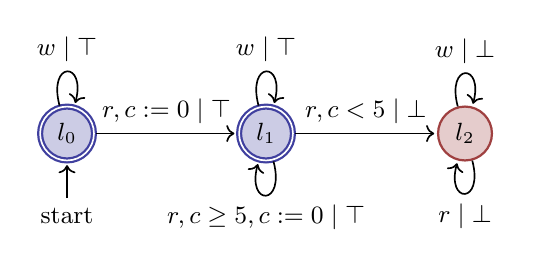
\begin{tikzpicture}[->,shorten >=1pt,auto,node distance=2cm, el/.style = {inner sep=2pt, align=left, sloped},
		every label/.append style = {font=\small},
		semithick,initial where=below]
		
		\tikzstyle{every node}=[font=\small]
		\tikzstyle{good state}=[circle,thick,draw=NavyBlue!75,fill=NavyBlue!20,minimum size=5mm,accepting]
		\tikzstyle{bad state}=[circle,thick,draw=Maroon!75,fill=Maroon!20,minimum size=3mm]
		\node[initial,good state] (l0) {$l_0$};
		\node[good state]         (l1) [right of=l0, xshift = 15pt] {$l_1$};
		\node[bad state]       (l2) [right of=l1, xshift = 15pt] {$l_2$};
  
		\path (l0) edge [loop above] node {$w \mid \green{\top}$} (l0)
		edge node { $r,c:=0 \mid \green{\top}$ } (l1)             
		(l1) edge [loop above] node {$ w \mid \green{\top}$} (l1)
		edge [loop below] node {$r, c \geq 5, c:=0 \mid \green{\top}$} (l1)
        edge node {$r,c<5 \mid \green{\bot}$} (l2)
		(l2) edge [loop above] node {$ w \mid \green{\bot}$} (l2)
             edge [loop below] node {$r\mid \green{\bot}$} (l2);
		\end{tikzpicture}%}
		\caption{Timed Transducer $\mathcal{A}_P$}
		\label{fig:TA}
	\end{figure}

 %    \begin{figure}[h]
	% 	\centering
 %        \begin{tikzpicture}[->,shorten >=1pt,auto,node distance=2cm, el/.style = {inner sep=2pt, align=left, sloped},
	% 	every label/.append style = {font=\small},
	% 	semithick,initial where=below]
		
	% 	\tikzstyle{every node}=[font=\small]
	% 	\tikzstyle{good state}=[circle,thick,draw=NavyBlue!75,fill=NavyBlue!20,minimum size=5mm,accepting]
	% 	\tikzstyle{bad state}=[circle,thick,draw=Maroon!75,fill=Maroon!20,minimum size=3mm]
	% 	\node[initial,good state] (l0) {$l_0$};
	% 	\node[good state]         (l1) [right of=l0, xshift = 15pt] {$l_1$};
	% 	% \node[bad state]       (l2) [right of=l1, xshift = 15pt] {$l_2$};
  
	% 	\path (l0) edge [loop above] node {$w \mid \green{\top}$} (l0)
	% 	edge node { $r,c:=0 \mid \green{\top}$ } (l1)             
	% 	(l1) edge [loop above] node {$ w \mid \green{\top}$} (l1)
	% 	edge [loop below] node {$r, c \geq 5, c:=0 \mid \green{\top}$} (l1)
 %        edge [loop right] node {$r,c<5 \mid \green{\bot_r}$} (l1);
	% 	% (l2) edge [loop above] node {$ w \mid \green{\bot}$} (l2)
 %  %            edge [loop below] node {$r\mid \green{\bot}$} (l2);
	% 	\end{tikzpicture}%}
	% 	\caption{Timed Transducer $\mathcal{A}_P$}
	% 	\label{fig:TA}
	% \end{figure}
    
% \saucomment{shall we change the output to 1 for all violating transitions and 0 for all accepting transitions?}
% \hscomment{yes}
        
 %    \subsection{Timed Automata}\label{sec:Timed Automata}
 %        As the STL formula under consideration will ultimately be transformed into a timed automaton in this paper, we provide the following preliminary details about timed automata.
        
 %        \paragraph{Timed Language}
 %        Let $\alphbt$ denote a finite alphabet. A pair $(t, a)\in\NonNegReals\times\alphbt$ is call an \emph{event}. A \emph{timed word} over $\alphbt$ is a finite sequence $\tword=(t_0,a_0)\cdots(t_n,a_n)\allowbreak\in(\NonNegReals\times\alphbt)^*$, where $t_i$ represents the global time when taking action $a_i$ for all $0\le i \le n$. A \emph{timed language} $\mathcal{L}$ is a set of timed word, i.e., $\mathcal{L}\subseteq(\alphbt\times\NonNegReals)^*$. Let $\emptyword$ denote the empty word.
        
 %        \paragraph{Timed automata}
	%     A Timed Automaton (TA) \cite{alur1994theory} is a kind of finite automaton equipped with a finite set of real-valued clocks. Let $\clock$ be the set of clock variables. A \emph{clock constraint} $g$ is a Boolean combinations of atomic constrains of the form $c\!\Join\!n$, with $c\in\clock$, $n\in\Nats$, \hscomment{can we replace this by $n\in\NonNegReals$?}and $\Join\in\{\le,<,\ge,>,=\}$. We use $\mathcal{G}(\clock)$ to denote the set of clock constraints. A \emph{clock valuation} $v:\clock\mapsto\NonNegReals$ is a function assigning a non-negative real value to each clock $c\in\clock$. We write $v\in g$ if the clock valuation $v$ satisfies the clock constraints $g$. For $d\in\NonNegReals$, let $v+d$ denote the clock valuation which maps every clock $c\in\clock$ to the value $v(c)+d$, and for a set $\mathcal{C}'\subseteq\clock$, let $\clockreset{\mathcal{C}'}$ denote the clock valuation which resets all clock variables in $\mathcal{C}'$ to $0$ and agrees with $v$ for other clocks in $\clock\setminus\{\mathcal{C}'\}$. Formally, a timed automaton is defined as below:

 %        \begin{definition}[Timed Automata]
 %            A timed automaton is a tuple $\automaton=(\alphbt,\loca,\linit,\lacpt,\clock,\trans)$, where
 %            \begin{itemize}
 %                \item $\alphbt$ is the alphabet;
 %                \item $\loca$ is a finite set of locations;
 %                \item $\linit$ is the initial location;
 %                \item $\lacpt\in\loca$ is a set of accepting locations;
 %                \item $\clock$ is the set of clocks;
 %                \item $\trans\subseteq \loca\times\alphbt\times\mathcal{G}(\clock)\times \power{\clock}\times \loca$ is a finite set of transitions. 
 %            \end{itemize}  
 %        \end{definition}

 %        \begin{example} (Timed automata).
 %    		\label{example:TA}
 %            The automaton $ \mathcal{A}_P $ in \cref{fig:TA} denotes a timed automaton of a prototype property $ P $ which says: "\textit{There should be a delay of at least 5 time units between any two user requests (r)}", with $ \loca=\{l_0,l_1,l_2\} $ as the set of locations, $ l_0 $ the initial location, and $\{l_0, l_1\}$ as the accepting locations (denoted by double circles). The alphabet of events is $ \Sigma=\{r,  \ldots\}$.  The automaton has one clock $c$. 
 %    	\end{example}
	% %\begin{wrapfigure}{r}{0.3\textwidth} 
 %    \begin{figure}[H]
	% 	\centering
	% 	%\scalebox{0.9}{
	% 	\begin{tikzpicture}[->,shorten >=1pt,auto,node distance=2cm, el/.style = {inner sep=2pt, align=left, sloped},
	% 	every label/.append style = {font=\small},
	% 	semithick,initial where=below]
		
	% 	\tikzstyle{every node}=[font=\small]
	% 	\tikzstyle{good state}=[circle,thick,draw=blue!75,fill=blue!20,minimum size=5mm,accepting]
	% 	\tikzstyle{bad state}=[circle,thick,draw=red!75,fill=red!20,minimum size=3mm]
	% 	\tikzstyle{dead state}=[rectangle,thick,draw=red!75,fill=red!20,minimum size=5mm]
	% 	\node[initial,good state] (l0) {$l_0$};
	% 	\node[good state]         (l1) [right of=l0] {$l_1$};
	% 	\node[dead state]       (l2) [right of=l1] {$l_2$};
  
	% 	\path (l0) edge [loop above] node {$\Sigma \setminus \{r\}$}( l0)
	% 	edge node { $r,c:=0$ } (l1)             
	% 	(l1) edge [loop above] node {$\Sigma \setminus \{r\}$} (l1)
	% 	edge [loop below] node {$r, c \geq 5, c:=0$} (l1)
 %        edge node {$r,c< 5$} (l2)
	% 	(l2) edge [loop above] node {$\Sigma$} (l2);		
	% 	\end{tikzpicture}%}
	% 	\caption{$ \mathcal{A}_P $}
	% 	\label{fig:TA}
	% %\end{wrapfigure}
	% \end{figure}


 %    The transitions can be understood as follows: from initial location $ l_0 $ and on the reception of input action $r$, $ \mathcal{A}_P$ makes a transition to location $ l_1 $ with the clock $ c $ being reset (to keep an eye on the reception of next $r$ action). From location $ l_1 $, if another action $r$ is received after 5 time unit, then $ \mathcal{A}_P  $ remains at the accepting location $l_1$ and resets its clock, otherwise goes to violating (non-accepting) location $l_2$.  From locations $l_0$ and $l_1$,  on input actions $\Sigma \setminus \{r\}$, $ \mathcal{A}_P $ remains at the same respective locations.
 
 % \begin{definition}[Semantics of TA]
	% 	\label{semTA}
	% 	The semantics of a TA is a timed transition system
	% 	 $\llangle \automaton \rrangle =( Q, q_0, \Gamma, \to, Q_F )$ 
 %        where the (infinite) set of states is given by $Q= L \times {\Bbb R}_{\geq0}^{|\clock|}$.
	% 	State $q_0=(l_0,v_0)$ is the initial state where $v_0$ is the	valuation that maps each clock in $\clock$ to $0$. The set of accepting states is given by $Q_F= F \times {\Bbb R}_{\geq0}^{|\clock|}$. The set of transition labels is given by
	% 	$\Gamma =  {\Bbb R}_{\geq0}\times \Sigma$. A label is a pair consisting of a delay (since the previous action) and an action.
	% 	The transition relation $\to\subseteq Q\times \Gamma\times Q$ is a set of transitions of the form $(l,v )\overset{{(\delta,a)}}{\longrightarrow} (l',v')$ with $\delta=t_n - t_{n-1}$ i.e., the difference between the absolute time of occurrence of action $a$ and the previous action and $v'=(v +\delta)[Y \leftarrow 0]$ whenever there exists $(l, g,a,Y, l') \in \Delta$  s.t. $v+\delta \models g$  for  $\delta\in {\Bbb R}_{\geq0}$.	
	% \end{definition}
        
        % \saucomment{we should add it somewhere else}\textcolor{red}{Our enforcer have the following properties:}
        % \begin{itemize}
        %     \item It will only modify the signal at the last time instants that the STL property is to be violated.
        % \end{itemize}
	%\noindent \textit{Deterministic and complete TA}. $\mathcal{A}$ is $deterministic$ whenever for any two distinct transitions $(l, g_1,a,Y_1, l_1')$ and $(l, g_2,a,Y_2, l_2')$ $\in \Delta$, $g_1\land g_2$ is unsatisfiable. ${\mathcal{A}}$ is $complete$ whenever for any location $l\in L$ and an action $a\in\Sigma$, the disjunction of the guards of the transitions leaving $l$ and labelled by $a$ evaluates to $true$. 

	%In this work, we only consider deterministic and complete TA \cite{alur1994theory,10.1016/j.scico.2016.02.008}. So, wherever we say a TA, it refers to a deterministic and complete TA.
     
        %\paragraph{Timed automata.} 
        
        
        
%
%
%        A clock valuation for $X$, where $X=\{x_1,\cdots,x_k\}$ is a finite set of clocks, is an element of ${\Bbb R}_{\geq0}^X$ , i.e., a function from $ X $ to ${\Bbb R}_{\geq0}^X$. $v+ \delta$ is the valuation assigning	$v(x) + \delta$ to each clock $ x $ of $ X $, where $ v \in  {\Bbb R}_{\geq0}^X$	and	$ \delta \in {\Bbb R}_{\geq0}$ (delay since previous action). Given a set of clocks $X'\subseteq X$, $v[X' \leftarrow 0]$ is the clock valuation $ v $ where all clocks in $ X' $ are assigned to 0. $ \mathcal{G}(X) $ denotes the set of guards. These are clock constraints defined as Boolean combinations of simple constraints of the form $ x \Join c $ with $ x \in X $, $ c \in {\Bbb N} $ and $\Join\in \{<,\leq,=,\geq,>\}$.	Given $g \in \mathcal{G}(X)$ and $v\in {\Bbb R}_{\geq0}^X$, we denote $v\models g$ when $ g $ holds according to $ v $. %\blue{A (semantic) state is a pair composed of a location and the clock valuations.}



    	% \begin{definition}[Timed automata]
    	% 	\label{def:ta}
    	% 	TA is a tuple ${\mathcal{A}}=(L, l_0, X, \Sigma,$ $\Delta, F)$, s.t. $L$ is a finite set of locations. $l_0 \in L$ is initial location. $X$ is a finite set of clocks. $\Sigma$ is a finite set of actions. $\Delta\subseteq L \times \mathcal{G}(X)\times \Sigma \times 2^X \times L$ is the transition relation. $F\subseteq L$ is the set of accepting locations.
    	% \end{definition}
	
    	


    %A run $ \rho $ from $ q \in Q $ is a sequence of moves in \sloppy{$ [\![ \calA ]\!]: \rho = q \xrightarrow{(\delta_1, a_1)} q_1 \cdots q_{n-1} \xrightarrow{(\delta_n, a_n)} q_n  $},	for some $ n \in N $, where the trace of a run $ \rho $ is the timed word $ (t_1, a_1) \cdot (t_2, a_2) \cdots (t_n, a_n) $, (where the date $t_n$ of action $ a_n $ is the sum of all the delays i.e., $ \Sigma_{i=1}^{n} \delta_i $). The set of runs from $ q_0 \in Q $ is denoted by $ Run(\calA) $. The subset of runs accepted by $ \calA $, i.e., when $ q_n \in F_G $ is denoted by $ Run_{F_G}(\calA) $. $\calL(\calA)$ denotes the language accepted by $\calA$ from its initial state $q_0$, whereas $\calL(\calA,q)$ denotes the language accepted by $\calA$ from state $q$.

    %%%%%%%%%%%%%%%%%%%%%%%%%%%%%%%%%%%%%%%%%%%%%%%%
    \subsection{Signal Temporal Logic}
    \label{sec:Signal Temporal Logic}
    %\paragraph*{Signal Temporal Logic} 
    Signal Temporal Logic (STL) \cite{maler2004monitoring} is a predicate logic used to describe and analyze continuous real-valued signals. Consider a signal $\signal:\NonNegReals\mapsto \Realn$. For each predicate $p(\signal)$, there is a corresponding function %\emph{linear function}
    $\mu_p:\Realn\mapsto \Reals$. The truth value of $p(\signal)$ at time $t$ is defined as follows:
    \begin{align*}
        p(\signal(t)) \Def\left\{
            \begin{aligned}
                \top,\quad \text{if}\quad \mu_p(\signal(t)) \ge 0,\\
                \bot,\quad \text{if}\quad \mu_p(\signal(t)) < 0.
            \end{aligned}\right.
    \end{align*}
    We will use the notion $p(\signal(t))\equiv\mu_p(\signal(t))\ge 0$ to define a predicate $p(x)$ in this paper. And we use \(|\signal|\) to denote the length of a signal.
    
    As demonstrated in \cite{fainekos2009robustness}, any STL formula can be equivalently converted into Negation Normal Form (NNF), in which negations appear only adjacent to predicates. In this paper, we considered \emph{non-nested} STL formula in NNF, which can be defined recursively as below:
    %this paper considers only the NNF representation of STL. The syntax of STL when expressed in NNF is outlined in the following definition:
    %\begin{definition}[STL in NNF Syntax]
    %\label{def:stl}
        %The syntax of Signal Temporal Logic (STL) is defined by
        %\saucomment{can we discuss this? Sure}
        \begin{align*}
            &\phi \Def ~ \top ~\mid~ p(\signal) ~\mid~ \neg p(\signal) ~\mid~ \phi_1 \land \phi_2 ~\mid~ \phi_1 \lor \phi_2,\\ %predicates
            &\varphi \Def ~ \phi_1 \until[I] \phi_2 ~\mid~ \phi_1 \release[I] \phi_2 ~\mid~ \varphi_1 \land \varphi_2 ~\mid~ \varphi_1 \lor \varphi_2~, %propositions
        \end{align*}
        where $\until_I$ and $\release_I$ are the \emph{until} and \emph{release} operators, respectively. $I=[t_1,t_2]$ is a \emph{bounded} interval with \emph{rational} endpoints (i.e., $t_1,t_2\in\NonNegRat$)\footnote{The endpoints of $I$ are restricted to $\NonNegRat$ to facilitate encoding this into the clock constraints of the TT defined in \cref{sec:Timed Transducer}}. Note that $\release_I$ are the dual of $\until_I$, in a way that $\phi_1\release_I\phi_2\equiv\neg(\neg\phi_1\until_I\neg\phi_2)$. We use $pd(\varphi)$ to denote the set of \emph{predicates} in an STL formula $\varphi$. The NNF replaces the negation of a formula by including all operators and their duals in the grammar. Other temporal operators can be defined as syntactic sugars, e.g., 
        %\[ 
            $\eventually_I\phi \equiv \top \until_I \phi,
            \always_I \phi \equiv \bot \release_I \phi$.
        %\]
    \begin{remark}
        We employ NNF because it facilitates the subsequent transformation of an STL formula into a timed transducer. This choice is strategically important since timed transducer, acting as a special form of timed automata, are not closed under complementation. Thus, negating an STL formula would necessitate taking the complement of its corresponding timed automaton, which is problematic due to this lack of closure. 
    \end{remark}

    The semantics of STL is defined as the satisfaction of a formula $\varphi$ with respect to a signal $\signal$ and time $t \in \NonNegReals$. 
        
        \begin{definition}[STL Semantics]
        \label{def:STL Semantics}
        The satisfaction of an STL formula $\varphi$ at a given time $t$ over a signal $\signal$, denoted by $(\signal, t) \models \varphi$, is inductively defined as follows:
            \begin{align*}
                &(\signal, t) \models \top & & \\
                &(\signal, t) \models p(x) & &\tiff\quad \mu_p(\signal(t)) \ge 0\\
                &(\signal, t) \models \neg p(x) & &\tiff\quad \mu_p(\signal(t)) < 0\\
                &(\signal, t) \models \varphi_1 \land \varphi_2& & \tiff\quad  (\signal, t) \models \varphi_1 \aand (\signal, t) \models \varphi_2\\
                &(\signal, t) \models \varphi_1 \lor \varphi_2& & \tiff\quad  (\signal, t) \models \varphi_1 \text{ or } (\signal, t) \models \varphi_2\\
                &(\signal , t) \models \varphi_1 \until_I \varphi_2& & \tiff\quad \exists t' \in t \oplus I,~ (\signal, t') \models \varphi_2\\ 
                & && \qquad\quad\aand\forall t'' \in [t, t'], (\signal, t'') \models \varphi_1\\
                & (\signal, t) \models \varphi_1 \release_I \varphi_2& & \tiff\quad \forall t'\in t \oplus I,~ (\signal, t') \models \varphi_2\\
                & && \qquad\quad\oor \exists t''\in[t,t'], (\signal,t'')\models \varphi_1
                %&\textcolor{red}{(\signal, t) \models \varphi_1 \release_I \varphi_2} && \tiff\quad (\exists t' \geq t, \suchthat (x,t') \models \varphi_1  \text{ and }\\ 
                %& && \qquad \qquad \forall t'' \geq t, \text{ such that } (x,t'') \models \varphi_2) \\
                %&&& \qquad \qquad \text{ or }  \forall t''' \geq t, (x, t''') \models \varphi_2
            \end{align*} 
            %φ R ψ is equivalent to ¬(¬φ U ¬ψ).
            % \hscomment{Release is dual to until, therefore it should be defined as above}
            % \saucomment{pl check above semantics of Release}
        \end{definition}
        %\hscomment{I feel there is no need to put is as remark}
        %\saucomment{yes, m putting this as a remark with a heading}
        %\begin{remark}[Relating Intervals in STL Formulas to Guards in Timed Transducer]    
            Intuitively, the subscript $I$ in the until operator $\until_I$ defines the timing constraints under which a signal must \emph{eventually} satisfy $\varphi_2$, while ensuring that $\varphi_1$ is satisfied beforehand. Similarly, the subscript $I$ in the release operator $\release_I$ specifies the timing constraints in which a signal must \emph{always} satisfy $\varphi_2$, unless $\varphi_1$ has been satisfied earlier. We say  $\signal\models\varphi$ if $(\signal,0)\models \varphi$.
        %\end{remark}
        
                \begin{example}
    		      \label{example:Properties in STL}
                The following examples illustrate some properties defined by STL.
                %For a signal $\signal$, we can think of various STL properties. For example:
    		    \begin{enumerate}
                    % \item $(\signal + 30 > 0 \land \signal - 30 < 0) \until_{[0,10]} (\signal = 100)$: The value of the signal will be 100 within 10 seconds; until then the value of the signal is within the range (-30,30).
                    \item $(\signal  \leq 30) \until_{[5,10]} (\signal = 0)$: The value of the signal will be $0$ at a time instant between $5$ to $10$ seconds; until then the value of the signal is less than $30$.
    		        \item $\always_{[0,\infty)} (\signal < 3.5)$: The signal is always below $3.5$.
                    \item $\eventually_{[0,30]} (\signal > 100)$: At some time in the first $30$ seconds, the value of the signal will exceed $100$. \qedT
    		    \end{enumerate}
    	    \end{example} 


    \subsection{Runtime Enforcement}
    \label{Preliminaries to Runtime Enforcement}
    The purpose of RE is to monitor input sequences produced by a running system and transform them into output sequences that adhere to a specified property $\varphi$. This is achieved using an enforcer.
 %This paper discusses RE of dense time signals. We can formally define an enforcer for a given property $\varphi$ as follows:
    % \hscomment{$\signal$ is a signal from $\NonNegReals$ to $\Realn$, and $X$ is the set of all such signal}
    
    \paragraph{Constraints on an Enforcer.} Let $X$ denote the set of signals \(\signal : \NonNegReals \mapsto \Realn\). Some constraints are required on how enforcer $E_{\varphi}$ for $\varphi$ transforms a signal $\signal$ at time $t$, to ensure that it performs correctly and minimally disruptively. %For example, the soundness constraint ensures that the enforcer’s output adheres to the specified property soundness. Without soundness, there would be no guarantee that the enforcer's output meets the desired specifications, undermining the purpose of runtime enforcement. 
    
    %Moreover, the transparency constraint ensures that the enforcer only intervenes when absolutely necessary. This is critical to maintaining system fidelity, as unnecessary modifications could disrupt expected behaviour, reduce efficiency, or introduce unintended side effects. By enforcing transparency, the enforcer maintains the integrity of the original signal as much as possible, preserving system performance and expected behaviour when no property violations occur. 
    
    %Lastly, the minimal/optimal modification constraint ensures that the enforcer modifies the output when the original input signal would violate the specified property such that it now satisfy the specified property and the modification should be minimal. By only making minimal changes, the enforcer keeps the output as close as possible to the original input signal. Overall, this constraint ensures that the enforcer is effective yet minimally invasive, thereby supporting system stability and efficiency. 
    % The formal definitions of the constraints are:
    

%   \hscommentinline{@Prof. Naijun, @Prof. Partha, @Prof. Srinivas: Please justified which version is more suitable}
    % \begin{definition}[Constraints on an Enforcer]\label{def:enforcer}
    %     Given an STL formula $\varphi$, an enforcer is a function $E_{\varphi}:X \times \NonNegReals \mapsto X$ that satisfies the following conditions:
    %     \begin{itemize}
    %         \item \emph{Soundness}:
    %         \[
    %         \forall \signal \in X,\forall t\in\NonNegReals,~ E_\varphi(\signal,t)=\resltsig \implies \resltsig\models \varphi,
    %         \]
    %         \item \emph{Transparency}:
    %         \[
    %         \forall \signal \in X,\forall t\in\NonNegReals, ~ \signal\models\varphi \implies  E_\varphi(\signal,t) = \signal,
    %         \]
    %         \item \emph{Minimal / optimal Modification}:
    %         \[
    %         \forall \signal \in X, \forall t\in\NonNegReals,~ \signal\not\models\varphi \implies E_\varphi(\signal,t) = \argmin_{\resltsig\in O}||\signal(t)-\resltsig(t)||,
    %         \]
    %         where $O = \{\resltsig\mid\resltsig\models \varphi\land |\signal|=|\resltsig|\}$, and $||\cdot||$ is the Euclidean norm in $\Realn$.
    %     \end{itemize}
    % \end{definition}

    % \saucomment{shall we have Def 5 with t or Def 6 without t?}
    % \nzcomment{I think this definition is correct, and the previous one is incorrect mathematically, at least not rigid enough.}
    \begin{definition}[Constraints on an Enforcer]\label{def:enforcer}
        Given an STL formula $\varphi$, an enforcer is a function $E_{\varphi}:X \mapsto X$ that satisfies the following conditions:
        \begin{itemize}
            \item \emph{Soundness}:
            \[
            \forall \signal \in X,~ E_\varphi(\signal)\models \varphi,
            \]
            \item \emph{Transparency}:
            \[
            \forall \signal \in X, ~ \signal\models\varphi \implies  E_\varphi(\signal) = \signal,
            \]
            \item \emph{Minimal Modification}:
            \[
            \forall \signal \in X,~ \signal\not\models\varphi \implies E_\varphi(\signal) = \argmin_{\resltsig\in O}||\signal-\resltsig||_s,
            \]
            where \(O = \{\resltsig \mid \resltsig \models \varphi \land |\signal| = |\resltsig|\}\), and $||\cdot||_s$ is the norm for signals defined as \(||\signal - \resltsig||_s \Def \max_t ||\signal(t) - \resltsig(t)||\), with $||\cdot||$ being the Euclidean norm in \(\Realn\).
        \end{itemize}
    \end{definition}
    
    %\saucomment{Note that: The "Minimal Modification" definition also includes instantaneity/ length preserving.}
    % Intuitively,  soundness.. transparency.. minimal modification..
    
    
    % Some constraints, namely soundness and transparency, are required on how enforcer $E_{\varphi}$ transforms signals $\signal$ at time $t$.
    
    % \begin{equation}
    %     Soundness: ~\forall \signal, \forall t \in \Reals_{\geq 0}, ~ E_{\varphi}(\signal,t)= \resltsig \implies \resltsig \models \varphi 
    % \end{equation}
    % Transparency
    % \begin{equation}
    %         Original ~signal:  \forall \signal, \forall t \in \Reals_{\geq 0}, \signal \models \varphi \implies E_{\varphi}(\signal,t)=\signal\\
    % \end{equation}
    % \begin{equation} 
    % \begin{split}
    %         Modified~ signal: \forall \signal, \forall t \in \Reals_{\geq 0}, \signal \not \models \varphi \implies\\ E_{\varphi}(\signal,t)=\resltsig: min(\mid\signal,\resltsig \mid) ~\land ~ \resltsig \models \varphi
    %         \end{split}
    % \end{equation}

    \begin{figure*}[htbp]
            \centering
            \begin{adjustbox}{max width=1\linewidth}
                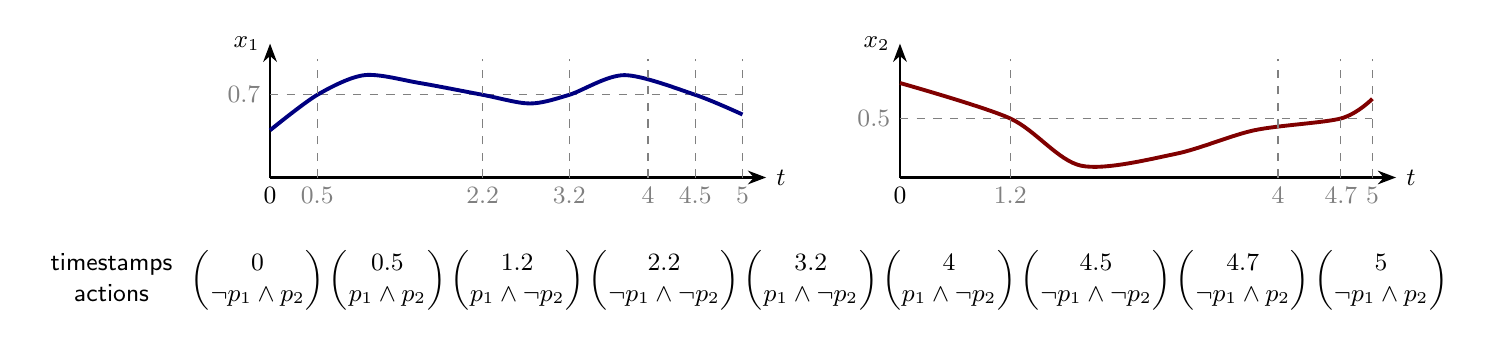
\begin{tikzpicture}[font=\small]
                    \centering
                    \begin{scope}
                        \draw[-Stealth, thick] (0,0) -- (6.3,0) node[right] {$t$};     
                        \draw[-Stealth, thick] (0,0) -- (0,1.7) node[above,left] {$x_1$};
                        \draw[dashed, color = gray] (0,1.05) node[left] {\black{$0.7$}} -- (6,1.05);
                        
                        \draw[color=NavyBlue, line width = 1.4pt, smooth, tension = 0.5] plot coordinates {
                            (0, 0.6)
                            (0.6, 1.05)
                            (1.2, 1.3)
                            (1.9, 1.2)
                            (2.7, 1.05)
                            (3.3, 0.94)
                            (3.8, 1.05)
                            (4.5, 1.3)
                            (5.4, 1.05)
                            (6.0, 0.8)
                        };
                        
                        \node at (0,0) [below] {\green{$0$}};
                        \draw[dashed, color = gray] (0.6, 0) node[below] {\orange{$0.5$}} -- (0.6,1.5);
                        \draw[dashed, color = gray] (2.7, 0) node[below] {\orange{$2.2$}} -- (2.7,1.5);
                        \draw[dashed, color = gray] (3.8, 0) node[below] {\orange{$3.2$}} -- (3.8,1.5);
                        \draw[dashed, color = gray] (4.8, 0) node[below] {\green{$4$}} -- (4.8,1.5);
                        \draw[dashed, color = gray] (5.4, 0) node[below] {\orange{$4.5$}} -- (5.4,1.5);
                        \draw[dashed, color = gray] (6,0) node[below] {\green{$5$}} -- (6,1.5);
                    \end{scope}

                    \begin{scope}[shift = {(8,0)}]
                        \draw[-Stealth, thick] (0,0) -- (6.3,0) node[right] {$t$};     
                        \draw[-Stealth, thick] (0,0) -- (0,1.7) node[above,left] {$x_2$};
                        \draw[dashed, color = gray] (0,0.75) node[left] {\black{$0.5$}} -- (6,0.75);

                        \draw[color=Maroon, line width = 1.4pt, smooth, tension = 0.5] plot coordinates {
                            (0, 1.2)
                            (1.4, 0.75)
                            (2.3, 0.15)
                            (3.5, 0.3)
                            (4.5, 0.6)
                            (5.6, 0.75)
                            (6.0, 1)
                        };

                        \node at (0,0) [below] {\green{$0$}};
                        \draw[dashed, color = gray] (1.4, 0) node[below] {\orange{$1.2$}} -- (1.4,1.5);
                        \draw[dashed, color = gray] (4.8, 0) node[below] {\green{$4$}} -- (4.8,1.5);
                        \draw[dashed, color = gray] (5.6, 0) node[below] {\orange{$4.7$}} -- (5.6,1.5);
                        \draw[dashed, color = gray] (6,0) node[below] {\green{$5$}} -- (6,1.5);
                    \end{scope}
                    
                    \node at(6,-1.3) {
                           $\begin{array}{c}
                                \textsf{timestamps}  \\
                                \textsf{actions}
                           \end{array}
                           \left(\!\!\!\begin{array}{c}
                               \green{0}  \\
                               \nblue{\neg p_1}\land \maroon{p_2} 
                          \end{array}\!\!\!\right) 
                          \left(\!\!\!\begin{array}{c}
                               \orange{0.5}  \\
                               \nblue{p_1}\land \maroon{p_2} 
                          \end{array}\!\!\!\right)
                          \left(\!\!\!\begin{array}{c}
                               \orange{1.2}  \\
                               \nblue{p_1}\land \maroon{\neg p_2} 
                          \end{array}\!\!\!\right)
                          \left(\!\!\!\begin{array}{c}
                               \orange{2.2}  \\
                               \nblue{\neg p_1}\land \maroon{\neg p_2} 
                          \end{array}\!\!\!\right)
                          \left(\!\!\!\begin{array}{c}
                               \orange{3.2}  \\
                               \nblue{p_1}\land \maroon{\neg p_2} 
                          \end{array}\!\!\!\right)
                          \left(\!\!\!\begin{array}{c}
                               \green{4}  \\
                               \nblue{p_1}\land \maroon{\neg p_2} 
                          \end{array}\!\!\!\right)
                          \left(\!\!\!\begin{array}{c}
                               \orange{4.5}  \\
                               \nblue{\neg p_1}\land \maroon{\neg p_2} 
                          \end{array}\!\!\!\right)
                          \left(\!\!\!\begin{array}{c}
                               \orange{4.7}  \\
                               \nblue{\neg p_1}\land \maroon{p_2} 
                          \end{array}\!\!\!\right)
                          \left(\!\!\!\begin{array}{c}
                               \green{5}  \\
                               \nblue{\neg p_1}\land \maroon{p_2} 
                          \end{array}\!\!\!\right)$
                    };
                \end{tikzpicture}
            \end{adjustbox}
            \caption{Signal Encoding against Formula $p_1\until_{[4,5]}p_2$}
            \label{fig:signal-encoding}
            \end{figure*}
            
    Intuitively, \emph{soundness} ensures that the output signal complies with the specified STL formula $\varphi$. \emph{Transparency} stipulates that if the input signal $\signal$ already meets $\varphi$, the enforcer should not alter it, but rather transmit the original signal $\signal$ as the output. \emph{Minimal modification} requires that if the input signal $\signal$ does not satisfy $\varphi$, the enforcer should adjust it to ensure compliance with $\varphi$, while keeping the modifications as minimal as possible relative to the original signal $\signal$.
    
    % Intuitively, \emph{soundness} means that the output signal satisfies the given STL formula $\varphi$. \emph{Transparency} means that if the input signal $\signal$ satisfies the given STL formula $\varphi$, then the enforcer should not modify it and simply relay the original signal $\signal$ as output. \emph{Minimal modification} means that if the input signal $\signal$ does not satisfy the given STL formula $\varphi$, then the enforcer should modify it such that it now satisfies the given STL formula $\varphi$ and the modification should be minimal with respect to the original signal $\signal$.


    %\hscommentinline{Transparency, Soundness, Enforcement Function, minimal modified function}


    
\paragraph{Problem Formulation}
\label{sec:Problem Formulation}
    %In this paper, we aim to construct a runtime enforcer for a given STL formula $\varphi$. Let $X$ denote the set of signals.  This enforcer takes as input signals $\signal \in X$ observed up to the current time $t$ and outputs modified signals $\resltsig$ that satisfy $\varphi$. 
    With all the preliminary details established, we now formally define the problem under consideration in this paper as follows:
    \begin{tcolorbox}[boxrule=.5pt,colback=white,colframe=black!75]
        \textbf{Synthesis of Enforcer.} Given an STL formula $\varphi$, construct an enforcer $E_{\varphi} : X \mapsto X$ for $\varphi$ that satisfies the \emph{soundness}, \emph{transparency}, and \emph{minimal modification} conditions as per \cref{def:enforcer}.
    \end{tcolorbox}

    % \begin{problem}
    %     Given an STL formula $\varphi$, construct an enforcer $E_{\varphi} : X \mapsto X$ of $\varphi$ that satisfies the soundness, transparency, and minimal modification conditions as per \cref{def:enforcer}.
    % \end{problem}

    % With all the priliminary be introduced, we now formally defined he problem under consideration in this paper as follows:
    % \begin{problem}
    %     % Given an STL formula $\varphi$, construct an enforcement function $E_{\varphi}:(X\times\NonNegReals)\mapsto X$, such that for all input signals $\signal$, the resulting signals $\resltsig=E_{\varphi}(\signal,t)$ satisfy: $\resltsig\vDash\varphi$.
    %     Given an STL formula $\varphi$, construct an enforcer $E_{\varphi}:X\mapsto X$ of $\varphi$ that satisfying the \emph{soundness}, \emph{transparency}, and \emph{minimal modification} conditions as per \cref{def:enforcer}.
    %     %such that for all input signals $\signal$, the resulting signals $\resltsig=E_{\varphi}(\signal,t)$ satisfy the constraints given in subsection \ref{Preliminaries to Runtime Enforcement} i.e., soundness and  transparency.
    % \end{problem} 

    % In order to solve this problem the approach that we employ is as follows: we will translate the given STL formula into timed transducer suitable for enforcement such that if a signal is accepted by the timed transducer, then it also satisfies the corresponding STL formula. We devise an enforcement algorithm (enforcer) that will yield the corrected signal (w.r.t. the given STL formula). This enforcer is \textit{Sound} (the output signal satisfies the given formula) and \textit{Transparent} (the input signal is modified when necessary and in a minimal way) with respect to the formula.
    % Having done this, at runtime, the given signal to be corrected is encoded as a timed word that is capable of being accepted by timed transducer.  %We then specify constraints on an enforcer and devise an enforcer or enforcement algorithm which is a solution to the specified constraints. 
    % That timed word is given as input to the algorithm, which enforces the formula (expressed as timed transducer) onto the signal. %encoded as a time word. 

    %  The steps can be recapitulated as follows:
    % \begin{enumerate}
    %     \item Signal Encoding: A signal should be encoded as a time word that is capable of being accepted by the timed transducer.
    %     \item Transform STL formula (to be enforced onto the given input signal) into the timed transducer.
    %     \item Enforcing the property expressed as a timed transducer onto the signal.
    % \end{enumerate}
    
    % The below sections explain these steps in detail.
    
\section{Signal Encoding}
\label{sec: Signal Encoding}

    % \begin{figure*}[htbp]
    %         \centering
    %         \begin{adjustbox}{max width=1\linewidth}
    %             \begin{tikzpicture}[font=\small]
    %                 \centering
    %                 \begin{scope}
    %                     \draw[-Stealth, thick] (0,0) -- (6.3,0) node[right] {$t$};     
    %                     \draw[-Stealth, thick] (0,0) -- (0,1.7) node[above,left] {$x_1$};
    %                     \draw[dashed, color = gray] (0,1.05) node[left] {\black{$0.7$}} -- (6,1.05);
                        
    %                     \draw[color=NavyBlue, line width = 1.4pt, smooth, tension = 0.5] plot coordinates {
    %                         (0, 0.6)
    %                         (0.6, 1.05)
    %                         (1.2, 1.3)
    %                         (1.9, 1.2)
    %                         (2.7, 1.05)
    %                         (3.3, 0.94)
    %                         (3.8, 1.05)
    %                         (4.5, 1.3)
    %                         (5.4, 1.05)
    %                         (6.0, 0.8)
    %                     };
                        
    %                     \node at (0,0) [below] {\green{$0$}};
    %                     \draw[dashed, color = gray] (0.6, 0) node[below] {\orange{$0.5$}} -- (0.6,1.5);
    %                     \draw[dashed, color = gray] (2.7, 0) node[below] {\orange{$2.2$}} -- (2.7,1.5);
    %                     \draw[dashed, color = gray] (3.8, 0) node[below] {\orange{$3.2$}} -- (3.8,1.5);
    %                     \draw[dashed, color = gray] (4.8, 0) node[below] {\green{$4$}} -- (4.8,1.5);
    %                     \draw[dashed, color = gray] (5.4, 0) node[below] {\orange{$4.5$}} -- (5.4,1.5);
    %                     \draw[dashed, color = gray] (6,0) node[below] {\green{$5$}} -- (6,1.5);
    %                 \end{scope}

    %                 \begin{scope}[shift = {(8,0)}]
    %                     \draw[-Stealth, thick] (0,0) -- (6.3,0) node[right] {$t$};     
    %                     \draw[-Stealth, thick] (0,0) -- (0,1.7) node[above,left] {$x_2$};
    %                     \draw[dashed, color = gray] (0,0.75) node[left] {\black{$0.5$}} -- (6,0.75);

    %                     \draw[color=Maroon, line width = 1.4pt, smooth, tension = 0.5] plot coordinates {
    %                         (0, 1.2)
    %                         (1.4, 0.75)
    %                         (2.3, 0.15)
    %                         (3.5, 0.3)
    %                         (4.5, 0.6)
    %                         (5.6, 0.75)
    %                         (6.0, 1)
    %                     };

    %                     \node at (0,0) [below] {\green{$0$}};
    %                     \draw[dashed, color = gray] (1.4, 0) node[below] {\orange{$1.2$}} -- (1.4,1.5);
    %                     \draw[dashed, color = gray] (4.8, 0) node[below] {\green{$4$}} -- (4.8,1.5);
    %                     \draw[dashed, color = gray] (5.6, 0) node[below] {\orange{$4.7$}} -- (5.6,1.5);
    %                     \draw[dashed, color = gray] (6,0) node[below] {\green{$5$}} -- (6,1.5);
    %                 \end{scope}
                    
    %                 \node at(6,-1.3) {
    %                        $\begin{array}{c}
    %                             \textsf{timestamps}  \\
    %                             \textsf{actions}
    %                        \end{array}
    %                        \left(\!\!\!\begin{array}{c}
    %                            \green{0}  \\
    %                            \nblue{\neg p_1}\land \maroon{p_2} 
    %                       \end{array}\!\!\!\right) 
    %                       \left(\!\!\!\begin{array}{c}
    %                            \orange{0.5}  \\
    %                            \nblue{p_1}\land \maroon{p_2} 
    %                       \end{array}\!\!\!\right)
    %                       \left(\!\!\!\begin{array}{c}
    %                            \orange{1.2}  \\
    %                            \nblue{p_1}\land \maroon{\neg p_2} 
    %                       \end{array}\!\!\!\right)
    %                       \left(\!\!\!\begin{array}{c}
    %                            \orange{2.2}  \\
    %                            \nblue{\neg p_1}\land \maroon{\neg p_2} 
    %                       \end{array}\!\!\!\right)
    %                       \left(\!\!\!\begin{array}{c}
    %                            \orange{3.2}  \\
    %                            \nblue{p_1}\land \maroon{\neg p_2} 
    %                       \end{array}\!\!\!\right)
    %                       \left(\!\!\!\begin{array}{c}
    %                            \green{4}  \\
    %                            \nblue{p_1}\land \maroon{\neg p_2} 
    %                       \end{array}\!\!\!\right)
    %                       \left(\!\!\!\begin{array}{c}
    %                            \orange{4.5}  \\
    %                            \nblue{\neg p_1}\land \maroon{\neg p_2} 
    %                       \end{array}\!\!\!\right)
    %                       \left(\!\!\!\begin{array}{c}
    %                            \orange{4.7}  \\
    %                            \nblue{\neg p_1}\land \maroon{p_2} 
    %                       \end{array}\!\!\!\right)
    %                       \left(\!\!\!\begin{array}{c}
    %                            \green{5}  \\
    %                            \nblue{\neg p_1}\land \maroon{p_2} 
    %                       \end{array}\!\!\!\right)$
    %                 };
    %             \end{tikzpicture}
    %         \end{adjustbox}
    %         \caption{Signal Encoding against Formula $p_1\until_{[4,5]}p_2$}
    %         \label{fig:signal-encoding}
            % \vskip\baselineskip
            
            % \begin{minipage}{.48\textwidth}
            %         \centering
            %         \begin{tabular}{c c c c}
            %             \toprule
            %             \textsf{clock} & \textsf{input} & \textsf{location after transition} & \textsf{output}  \\
            %             \midrule
            %              0   & $\neg p_1\land p_2$ & $l_1$ & $\bot_1$ \\
            %              0.5 & $ p_1\land p_2 $     & $l_1$ & $\top$   \\
            %              1.2 & $ p_1\land\neg p_2 $ & $l_1$ & $\top$   \\
            %              2.2 & $\neg p_1\land \neg p_2 $ & $l_1$ & $\bot_1$ \\
            %              3.2 & $p_1\land \neg p_2 $     & $l_1$ & $\top$   \\
            %              4   & $p_1\land \neg p_2 $     & \red{$l_3$} & $\top$   \\
            %              4.5 & $\neg p_1\land \neg p_2 $  & $l_3$ & $\bot_1$   \\
            %              4.7 & $\neg p_1\land p_2 $     & \red{$l_2$} & $\bot_1$\\  
            %              \bottomrule
            %         \end{tabular}
            %         \captionof{table}{Enforcement of timed word  obtained from Figure \ref{fig:signal-encoding} using Until Transducer}
            %         \label{tab:table_enf}
            % \end{minipage}
            % \hfill
            % \begin{minipage}{.48\textwidth}
            %     \centering
            %     \begin{tikzpicture}
            %         \centering
            %         \begin{scope}
            %             \draw[-Stealth, thick] (0,0) -- (6.3,0) node[right] {$t$};     
            %             \draw[-Stealth, thick] (0,0) -- (0,1.7) node[above,left] {$\signal_1$};
            %             \draw[dashed, color = gray] (0,1.05) node[left] {\black{$0.7$}} -- (6,1.05);
                        
            %             \draw[color=NavyBlue, line width = 1.4pt, smooth, tension = 0.5] plot coordinates {
            %                 %(0, 0.75)
            %                 (0.6, 1.05)
            %                 (1.2, 1.3)
            %                 (1.9, 1.2)
            %                 (2.7, 1.05)};
            %                 %(3.3, 0.94)
            %             \draw[color=NavyBlue, line width = 1.4pt, smooth, tension = 0.5] plot coordinates {
            %                 (3.8, 1.05)
            %                 (4.5, 1.3)
            %                 (5.4, 1.05)
            %                 %(6.0, 0.8)
            %             };
            %             \draw[color=red, line width = 1.6pt] plot coordinates{(0,1.05) (0.6,1.05)};
            %             \draw[color=red, line width = 1.6pt] plot coordinates{(2.7,1.05) (3.8,1.05)};
            %             \draw[color=red, line width = 1.6pt] plot coordinates{(5.4,1.05) (5.6,1.05)};
                        
            %             \node at (0,0) [below] {\green{$0$}};
            %             \draw[dashed, color = gray] (0.6, 0) node[below] {\orange{$0.5$}} -- (0.6,1.5);
            %             \draw[dashed, color = gray] (2.7, 0) node[below] {\orange{$2.2$}} -- (2.7,1.5);
            %             \draw[dashed, color = gray] (3.8, 0) node[below] {\orange{$3.2$}} -- (3.8,1.5);
            %             \draw[dashed, color = gray] (4.8, 0) node[below] {\green{$4$}} -- (4.8,1.5);
            %             \draw[dashed, color = gray] (5.4, 0) node[below] {\orange{$4.5$}} -- (5.4,1.5);
            %             \draw[dashed, color = gray] (6,0) node[below] {\green{$5$}} -- (6,1.5);
            %         \end{scope}

            %         \begin{scope}[shift = {(0,-2.3)}]
            %             \draw[-Stealth, thick] (0,0) -- (6.3,0) node[right] {$t$};     
            %             \draw[-Stealth, thick] (0,0) -- (0,1.7) node[above,left] {$\signal_2$};
            %             \draw[dashed, color = gray] (0,0.75) node[left] {\black{$0.5$}} -- (6,0.75);

            %             \draw[color=Maroon, line width = 1.4pt, smooth, tension = 0.5] plot coordinates {
            %                 (0, 1.2)
            %                 (1.4, 0.75)
            %                 (2.3, 0.15)
            %                 (3.5, 0.3)
            %                 (4.5, 0.6)
            %                 (5.6, 0.75)
            %                 (6.0, 1)
            %             };

            %             \node at (0,0) [below] {\green{$0$}};
            %             \draw[dashed, color = gray] (1.4, 0) node[below] {\orange{$1.2$}} -- (1.4,1.5);
            %             \draw[dashed, color = gray] (4.8, 0) node[below] {\green{$4$}} -- (4.8,1.5);
            %             \draw[dashed, color = gray] (5.6, 0) node[below] {\orange{$4.7$}} -- (5.6,3.8);
            %             \draw[dashed, color = gray] (6,0) node[below] {\green{$5$}} -- (6,1.5);
            %         \end{scope}
                     
            %     \end{tikzpicture}
            %     \caption{Signal After Enforcement}
            %     \label{fig:after-enforce}
            % \end{minipage}
        % \end{figure*}
    In this section, we will introduce the procedure for encoding a signal into a timed word. This step is essential because we aim to enforce a signal using a TT, but a signal, defined as a real-valued function over dense time, is not directly compatible with TT. 
    %A signal, defined as a real-valued function over dense time, is not directly compatible with transducers. To bridge this gap, we introduce a procedure to encode the signal into a timed word, which is accepted by a transducer. 
    
    The encoding process, applied to a given signal $\signal$ with respect to an STL formula $\varphi$, involves recording the truth value of predicates of $\varphi$ at both \emph{variable points} and \emph{relevant points} within the signal. We will now provide a detailed explanation of this encoding procedure.

    \paragraph{Variable Points}
    Intuitively, a variable point is where the truth value of a predicate regarding the signal changes.
        The concept of variable points is as below.
        \begin{definition}[Variable Point \customcite{bae2019bounded}{Def.~2.8}]
            Given a signal $\signal:\NonNegReals \mapsto \Realn$, a time point $\tau\in \NonNegReals$ is a variable point of $\signal$ with respect to a predicate $p(\signal)$ if for some neighborhood $B$ containing $\tau$, there are different truth values $u$ and $v$ such that $p(\signal)=u$ for every $t\in B\cap [0,\tau)$ and $p(\signal)=v$ for every $t\in B\cap (\tau,+\infty)$.
        \end{definition} 

        
        
        In this paper, we limit our focus to \emph{non-Zeno} signals constrained within a \emph{bounded} time frame. Consequently, such signals possess a finite number of variable points. There is a notable characteristic of variable points, formalized in the following proposition:
        \begin{proposition}
            Given a signal $\signal$ and a predicate $p(\signal)$, assume $t_0 < t_1 < \cdots < t_k$ denote all the variable points of $\signal$ with respect to $p(\signal)$. It is then established that the truth value of $p(\signal)$ remains constant within each open interval $(t_i, t_{i+1})$ for all indices $i = 0, 1, \ldots, k$\footnote{Here, $t_{k+1}$ is defined to be the endpoint of the signal $\signal$.}.
        \end{proposition}

        Consequently, the signal $\signal$ can be effectively encoded as a timed word:
        \[
            \tword = (t_0, a_0), (t_1, a_1), \cdots, (t_k, a_k),
        \]
        where each $t_i$ denotes a variable point with respect to $p(\signal)$, and each $a_i$ represents the truth value of $p(\signal)$ within the interval $(t_i, t_{i+1})$ for indices $i = 0, 1, \ldots, k$. This encoding method ensures that $\tword$ comprehensively captures all information about $\signal$ with respect to the predicate $p(\signal)$. 

        The set of variable points of a signal with respect to an STL formula $\varphi$ is defined as the union of the sets of variable points for all predicates $p\in pd(\varphi)$\footnote{Recall that $pd(\varphi)$ is defined as the set of predicates in an STL formula $\varphi$ in \cref{sec:Preliminaries and notations}}. Accordingly, the timed word can be constructed based on these combined variable points. 
    %
        The following example provides a comprehensive illustration of this process:

        \begin{example}\label{exp:variable-point}
            Consider the signal $\signal=(x_1, x_2)$ illustrated in \cref{fig:signal-encoding}, and the STL formula $\varphi = p_1 \until_{[4,5]} p_2$, with $p_1 \equiv x_1 - 0.7 \ge 0$, and $p_2 \equiv x_2 - 0.5\ge 0$. The time word for $\signal$ with respect to $\varphi$ is given by:
            \begin{align*}
            &(0.5,p_1\land p_2),(1.2, p_1 \land \neg p_2),(2.2, \neg p_1\land \neg p_2),(3.2, p_1\land \neg p_2),&&\\
            &(4.5,\neg p_1\land \neg p_2), (4.7, \neg p_1 \land p_2)%\qquad\qquad\qquad\qquad\qquad
            &&\lhd
            \end{align*}
            %\qedT
        \end{example}
        %\hscomment{The procedure of computing the variable point is given here.}
        
        The values of a signal \(\signal\) that may lead to variable points against the predicate \(p(\signal)\) can be determined by solving the equation \(\mu_p(x)=0\). Depending on the structure of $\mu_p(x)$, different methods can be used to find or approximate the root of $\mu_p(x)$:
        \begin{enumerate*}[label=(\roman*)]
            \item Gaussian elimination is suitable for linear forms of $\mu_p(x)$,
            \item Newton-Raphsom method can be used for polynomial forms of $\mu_p(x)$,
            \item For more complex forms, such as transcendental equations, the Real roots isolation method \cite{gan2017reachability} can be used to approximate the intervals of the roots.
        \end{enumerate*}
        Using $vv(p)$ to denote the set of such valuations against predicate $p$, then $vv(\varphi) = \cup_{p\in pd(\varphi)}vv(p)$ for a given STL formula $\varphi$.  
        
        Variable points are effective for documenting changes in a signal in accordance with a specific STL formula. However, they may not provide sufficient information for \emph{enforcing} compliance with an STL property.
        Consider, for example, the scenario depicted in \cref{exp:variable-point}, where the proposition $p_1$ is false within the time interval $[0,0.5)$. This condition leads to the STL formula $\varphi$ not being satisfied by the signal $\signal$. However, in the absence of an input event before $t=0.5$ — specifically, an input at $t=0$ — no transducer can confirm that $\varphi$ is unsatisfied by the signal, nor can it enforce the signal accordingly.
        To address this, it becomes necessary to incorporate \emph{relevant points} tailored to an STL formula, ensuring all relevant events are recorded. %\nzcomment{We may need to discuss how to compute the set of variable points for a given STL formula and a set of signals, which depends on the structure of the formulas and the signals.}

        
        \paragraph{Relevant Points} Intuitively, relevant points include the time points that correspond to the interval boundaries of the given formula and the initial instant of the given signal. These points mark where the satisfaction requirements for predicates may change. For example, in the formula \( p_1 \until_{[t_1,t_2]} p_2 \), before \(t_1\), ensuring that \(p_1\) is satisfied suffices. However, after \(t_1\), it is also necessary to verify the satisfaction of \(p_2\).
        
        We proceed to inductively define relevant points of an STL formula as follows:
            \begin{definition}[Relevant Point]
                Given an STL formula $\varphi$, the set of relevant points $rp(\varphi)$ is inductively defined by:
                \begin{gather*}
                rp(\top) = \emptyset,\quad rp(\varphi_1\land\varphi_2) = rp(\varphi_1)\cup rp(\varphi_2),\\ %assuming \varphi_1 is until, etc.
                rp(p(x)) = \{ 0 \},\quad rp(\varphi_1\lor\varphi_2) = rp(\varphi_1)\cup rp(\varphi_2),\\
                rp(\varphi_1\until_{[t_1,t_2]}\varphi_2) = \{t_1,t_2\}\cup rp(\varphi_1) \cup rp(\varphi_2),\\
                rp(\varphi_1\release_{[t_1,t_2]}\varphi_2) = \{t_1,t_2\}\cup rp(\varphi_1)\cup rp(\varphi_2).
                \end{gather*}
            \end{definition}

            % Intuitively, relevant points include the time points that correspond to the interval boundaries of the given formula and the initial instant of the given signal. These points mark where the satisfaction requirements for predicates may change. For example, in the formula \( p_1 \until_{[t_1,t_2]} p_2 \), before \(t_1\), ensuring that \(p_1\) is satisfied suffices. However, after \(t_1\), it is also necessary to verify the satisfaction of \(p_2\).
            
            % Intuitively, relevant points contain the time points that correspond to the interval boundary of the given formula and the initial instant of the given signal. 
            % These are the points where satisfaction requirements of the predicates may change. Such as for $p_1\until_{[t_1,t_2]}p_2$, before $t_1$, only $p_1$ show be ensure to be satisfied, but after $t_1$, we also need to check about the satisfaction of $p_2$.
            
            % These are the points where we need to make sure that the signal, if not satisfying the respective predicates in the formula, then definitely satisfy the predicates during enforcement. 
            
            The actions of events at time points $t \in rp(\varphi)$ reflect the truth values of all predicates in $\varphi$ at time $t$, which can be directly sampled in real-time from the signal. Consider the following example for further illustration:
            
            \begin{example}\label{exp:relavant-point}
                Continuing \cref{exp:variable-point}, recall that $\varphi=p_1\until_{[4,5]}p_2$. The set of relevant point $rp(\varphi)=\{0,4,5\}$, and the events at relevant points with respect to signal $\signal=(x_1,x_2)$ is:
                \begin{align*}
                    (0,\neg p_1\land p_2),(4, p_1\land \neg p_2),(5,\neg p_1\land p_2).
                \end{align*}
                Consequently, the complete time word encoded from $\signal$ with respect to the STL formula $\varphi$ is depicted in \cref{fig:signal-encoding}. The events at variable points are highlighted in orange, while the events at relevant points are marked in green.
                \qedT
            \end{example}

        \paragraph{Signal encoding} We now give the process of signal encoding. 
        The signal encoding process, as outlined in \cref{alg:signal-encoding}, operates in real-time by monitoring changes in the truth values of predicates within the given STL formula. In an infinite loop, the algorithm waits for the input signal (\cref{line:await}) at current time $t$ (the function \textsf{current\_time()} can be used to get the current time as shown in \cref{line:time}). It updates the truth values \texttt{CurrPred} of all predicates (\cref{line:update value}) with respect to the current signal values. An event is emitted (\cref{line: emit}) whenever a variable point or relevant point is met (\cref{line:if condition}). 
        %The identification of variable points is achieved by comparing the truth value \texttt{PrevPred} in the previous loop with the current truth value \texttt{CurrPred} (the condition $\texttt{CurrPred}\neq \texttt{PrevPred}$ in the line \ref{line:if condition}).

    %     \hscomment{how to update the time $t$ in \cref{alg:signal-encoding} should be clarify}
    %     \begin{algorithm}[H]
    %     \caption{$\textsf{SignEncode}(\signal,\varphi)$}
    %     \label{alg:signal-encoding} %\scriptsize
    %     \begin{algorithmic}[1]
    %         \Require $\signal$: signal, $\varphi$: STL formula
    %         \Ensure $\sigma$: time word encoded from $\signal$
    %         \State $\texttt{Rele} \gets rp(\varphi)$, $\texttt{Pred} \gets pd(\varphi)$ 
    %         \State $\texttt{CurrPred} \gets [False,\cdots,False]$ 
    %         \State $\texttt{PrevPred} \gets [False,\cdots,False]$
    %         \While {await\_signal} 
    %             \State Update current time $t$  \label{line:update time}
    %             \State $\texttt{CurrPred}\gets$ Truth values of predicates $p\in \texttt{Pred}$ with respect to $\signal$ at $t$\label{line:update value}
    %             \If{$\texttt{CurrPred}\neq \texttt{PrevPred}$ or $t\in \texttt{Rele}$} \label{line:if condition}
    %                 \State Emit $(t,\texttt{CurrPred})$ \label{line: emit}
    %             \EndIf
    %             \State $\texttt{PrevPred}\gets \texttt{CurrPred}$
    %         \EndWhile
    %     \end{algorithmic}
    % \end{algorithm}
    \begin{algorithm}[H]
        \caption{$\textsf{SignEncode}(\varphi)$}
        \label{alg:signal-encoding} %\scriptsize
        \begin{algorithmic}[1]
            \Require $\varphi$: STL formula
            \Ensure $\sigma$: time word encoded from $\signal$
            \State $\texttt{Rele} \gets rp(\varphi)$, $\texttt{Vari} \gets vv(\varphi)$,  $\texttt{Pred} \gets pd(\varphi)$ 
            %\State $\texttt{CurrPred} \gets [False,\cdots,False]$ 
            %\State $\texttt{PrevPred} \gets [False,\cdots,False]$
            \While {true}
                \State $\signal$ $\gets$ \textsf{await\_signal}() \label{line:await}
                \State $t$ $\gets$ \textsf{current\_time}() \label{line:time} \Comment{Get the current time $t$}
                \State $\texttt{CurrPred}\gets$ Truth values of predicates $p\in \texttt{Pred}$ with respect to $\signal$ at $t$\label{line:update value}
                %\If{$\texttt{CurrPred}\neq \texttt{PrevPred}$ or $t\in \texttt{Rele}$} \label{line:if condition}
                \If{$\signal(t)\in\texttt{Vari}$ or $t\in\texttt{Rele}$}\label{line:if condition}
                    \State Emit $(t,\texttt{CurrPred})$ \label{line: emit}
                    %\State Emit $(t,)$
                \EndIf
                %\State $\texttt{PrevPred}\gets \texttt{CurrPred}$
            \EndWhile
        \end{algorithmic}
    \end{algorithm}

    \begin{remark}
        During the signal encoding process, we can proactively identify variable points and relevant points, allowing for the enforcement of the signal before any actual violations occur. This proactive enforcement can be achieved by:
        \begin{enumerate*}[label=(\roman*)]
            \item expanding the values at a variable point into its surrounding neighborhood, and
            \item slightly adjusting the timing of relevant points in $rp(\varphi)$ to check these points in advance.
        \end{enumerate*}
    \end{remark}

    
    %In \cref{alg:signal-encoding}, $Rele$ is the set of relevant points. $Pred$ is set of  predicates included in the STL formula $\varphi$. Initially, the current and previous truth values of all the predicates with respect to $\signal$ is set to $False$, i.e., $CurrPred \gets [False,\cdots,False]$ and $Prevpred \gets [False,\cdots,False]$. Upon receiving a signal, the (current) truth values of all the predicates is found out. If those changed, then the truth values of the predicates are emitted (as a timed event) along with the current time. Also, if the current time point is a relevant point, then the truth values of the predicates at the current relevant point are emitted (as a timed event) along with the current time.
    % In order to enforce the signal using TA, we need first encode the continuous signal into timed word, which can be accepted by a TA.
    
    % The given signals, to be corrected, $\signal_1, \cdots, \signal_k$ should be encoded as a time word that is capable of being accepted by a timed transducer.
    % The first step is: for each given signal, we extract the variable points. 
    %for the given signal we extract the variable points. For a signal $\signal: D \mapsto \Realn$, a time point $\tau\in D$ is called a \emph{variable point} if the truth value of a proposition changes at time $\tau$ on the signal $\signal$. we take all the variable points with the truth value of the preposition and constitute the primary timed word. however this is not the final encoding of a signal to be relayed to the transducer. we need to carefully observer (and modify/enforce) the signal at the interval boundaries if the signals do not satisy the given STL formula. why at boundaries, because we want to modify the signals  just before the point after which it can no longer be corrected. thus we account those boundary time points into our timed word. and this gives our final timed word representing a signal. we take an example  where given signals and STL specifications, we explain how  we get the final timed word below.
    
    
    
    % \paragraph*{Variable point.} For a signal $\signal: D \mapsto \Realn$, a time point $\tau\in D$ is called a \emph{variable point} if the truth value of a proposition changes at time $\tau$ on the signal $\signal$.
    
    % \begin{definition}[Variable Point\cite{bae2019bounded}]
    %     Given a signal $\signal:D\mapsto \Realn$, a time point $\tau\in D$ is a variable point of $\signal$ with respect to a proposition $\mu(\signal)$ if for some neighborhood $B\ni \tau$, there are different truth values $u$ and $v$ such that $\mu(\signal)=u$ for every $t\in B\cap [0,\tau)$ and $\mu(\signal)=v$ for every $t\in B\cap (\tau,+\infty)$.
    % \end{definition} 

    % \begin{remark}
    %     In this work, we consider bounded signals: the domain and the number of variable points are bounded. 
    % \end{remark}
    
    % We gather all the variable points along with the truth value of the proposition at those points to form the primary timed word. However, this is not the final encoding of the signal to be relayed to the transducer.  We need to carefully observe (and potentially modify or enforce) the signal at the interval boundaries if the signals do not satisfy the given STL formula. Why at boundaries? Because we want to correct the signal just before the point after which correction is no longer possible. Thus, we account for these boundary time points in our timed words.
    % And doing this provides the final timed word representing a signal and suitable to be relayed to the transducer. 

    % So, for the given signals $\signal_1, \cdots, \signal_k$, the corresponding timed word $\tword$ follows these:
    % \begin{itemize}
    %     \item Each time point in $\tword$ is a variable point of at least one signal from $\signal_1, \cdots, \signal_k$;
    %     \item The alphabet in each event $(\tau_i,\mu)$ is similar to the satisfaction of the proposition in $B\cap(\tau_i,+\infty)$, where $B$ is a small enough neighbourhood where the truth value of all the signals change. 
    % \end{itemize}

    
    % Below, given signals and STL specification, we explain how we obtain the final timed word via an example.

    % \begin{example}[Extracting Variable points from the signal]
    % Given an STL formula $(\signal_1\ge 0.7)\until_{[4,5]}(\signal_2\ge 0.5)$, with $p_1\equiv \signal_1\ge 0.7$, $p_2\equiv \signal_2 \ge 0.5$ and signals $\signal_1$ and $\signal_2$  given in Figure \ref{fig:signal-encoding}, we extract the variable points $(\neg p_1 \land p_2, 0), (p_1 \land p_2, 0.5), (p_1 \land \neg p_2, 1.2), (\neg p_1 \land \neg p_2, 2.2), (p_1 \land \neg p_2, 3.2), (\neg p_1 \land \neg p_2, 4.5) \text{ and } (\neg p_1 \land p_2, 4.7)$ as marked (in colour red) in the plots of the Figure \ref{fig:signal-encoding}. This constitutes our primary timed word. Now, the points at the interval boundaries should also be considered. So, the final timed word is \sloppy $(\neg p_1 \land p_2, 0), (p_1 \land p_2, 0.5), (p_1 \land \neg p_2, 1.2), (\neg p_1 \land \neg p_2, 2.2), (p_1 \land \neg p_2, 3.2), (p_1 \land \neg p_2, 4),(\neg p_1 \land \neg p_2, 4.5), (\neg p_1 \land p_2, 4.7) \text{ and } (\neg p_1 \land p_2, 5)$ where the interval boundary points are $(p_1 \land \neg p_2, 4), (\neg p_1 \land p_2, 5)$ marked (in colour green) in the plots of the Figure \ref{fig:signal-encoding}. This constitutes our final timed word.
    %For a given signal of humidity in the top plot in Figure \ref{} and for the given proposition $\varphi \geq 55$, the variable points (humidity crossing 55\%) are shown (marked by red dots) in the bottom plot in Figure \ref{}. 
    %     \begin{figure*}[p]
    %         \centering
    %         \includegraphics[width=1\linewidth]{figures/variable_points.png}
    %         \caption{Extracting Variable points from the signal)}
    %         \label{fig:enter-label}
    %     \end{figure*}        
    % \end{example}


\section{Constructing Timed Transducer from STL}
\label{sec: Transform STL into TA}

    \begin{figure*}[t]
        \begin{minipage}{.48\textwidth}
            \centering
            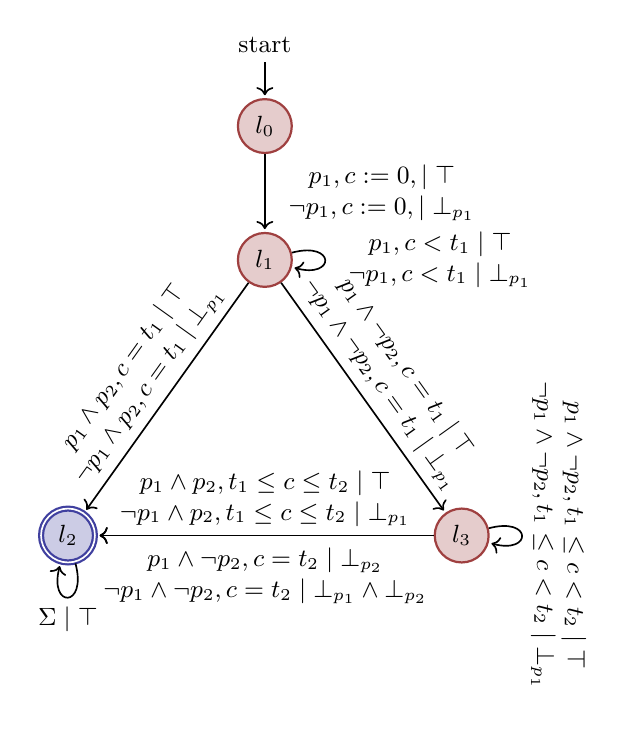
\begin{tikzpicture}[->,shorten >=1pt,auto,node distance=3.5cm,el/.style = {inner sep=2pt, align=left, sloped},every label/.append style = {font=\scriptsize},semithick,initial where=above]
			
			\tikzstyle{every node}=[font=\small]
			\tikzstyle{good state}=[circle,thick,draw=NavyBlue!75,fill=NavyBlue!20,minimum size=5mm,accepting]
			\tikzstyle{bad state}=[circle,thick,draw=Maroon!75,fill=Maroon!20,minimum size=3mm]
			\tikzstyle{dead state}=[rectangle,thick,draw=Maroon!75,fill=Maroon!20,minimum size=5mm]

                \node[initial, bad state]  at (0,-0.3) (S0) {$l_0$};
                \node[bad state] at (0,-2) (S2) {$l_1$};
			\node[good state] at (-2.5,-5.5)  (S3) {$l_2$};
			\node[bad state] at (2.5,-5.5)  (S4)  {$l_3$};
			
			\path (S0) edge node {$\begin{array}{c}
                                    p_1, c:=0, \mid \green{\top}\\ 
                                    \neg p_1, c:=0, \mid \green{\bot_{p_1}}  
                                    \end{array}$}(S2)
            
                      (S2) edge [loop right] node  {$\begin{array}{c} 
                                    p_1, c<t_1 \mid \green{\top} \\
                                    \neg p_1, c<t_1 \mid \green{\bot_{p_1}} \end{array}$} 
                      (S2) edge node [el,above] {$\begin{array}{c}
                                    p_1 \land p_2, c = t_1 \mid \green{\top}\\
                                    \neg p_1 \land p_2, c = t_1 \mid \green{\bot_{p_1}}\end{array}$} 
                      (S3) edge node [el,above] {$\begin{array}{c}
                                    p_1 \land \neg p_2, c=t_1 \mid \green{\top}\\
                                    \neg p_1 \land \neg p_2, c=t_1 \mid \green{\bot_{p_1}} \end{array}$} 
                      (S4)
			         (S3) edge [loop below] node {$\Sigma \mid  \green{\top}$} (S3)
            
                      (S4) edge [loop right] node [el,above] {$\begin{array}{c}
                                    p_1 \land \neg p_2, t_1 \le c < t_2 \mid \green{\top}\\ 
                                    \neg p_1 \land \neg p_2, t_1 \le c < t_2 \mid \green{\bot_{p_1}}  \end{array}$} 
                      (S4) edge node [el,above]{$\begin{array}{c} 
                                    p_1 \land p_2, t_1 \le c \leq t_2 \mid \green{\top}\\
                                    \neg p_1 \land p_2, t_1 \leq c \leq t_2 \mid \green{\bot_{p_1}}\end{array}$} (S3)
                      (S4) edge node {$\begin{array}{c}
                                    p_1 \land \neg p_2, c = t_2 \mid \green{\bot_{p_2}}\\
                                    \neg p_1 \land \neg p_2, c=t_2 \mid \green{\bot_{p_1}\land\bot_{p_2}}\end{array} $} (S3);
		\end{tikzpicture}
            \vspace{-.6cm}
            \caption{Timed Transducer $\automaton_{\until}$}
            \label{fig: until}
        \end{minipage}
        \hfill
        \begin{minipage}{.48\textwidth}
            \centering
            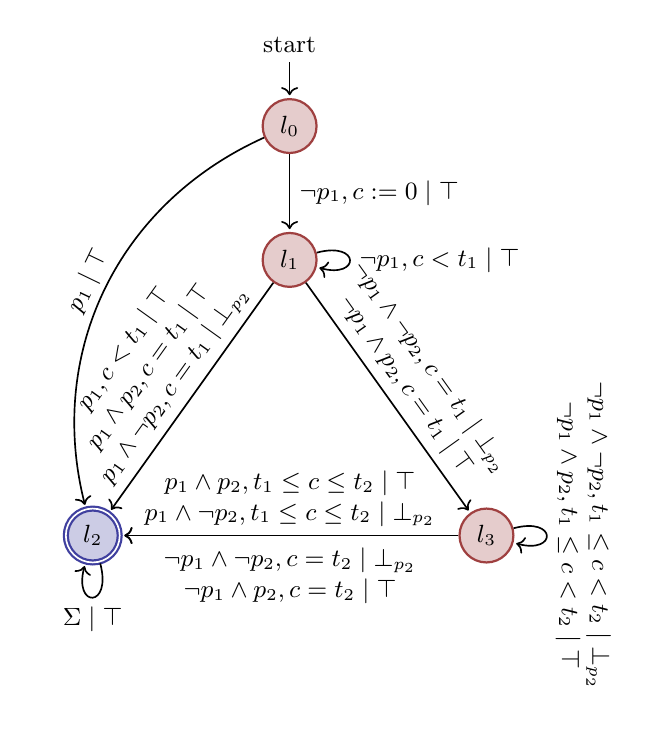
\begin{tikzpicture}[->,shorten >=1pt,auto,node distance=3.5cm,el/.style = {inner sep=2pt, align=left, sloped},every label/.append style = {font=\scriptsize},semithick,initial where=above]
			
			\tikzstyle{every node}=[font=\small]
			\tikzstyle{good state}=[circle,thick,draw=NavyBlue!75,fill=NavyBlue!20,minimum size=5mm,accepting]
			\tikzstyle{bad state}=[circle,thick,draw=Maroon!75,fill=Maroon!20,minimum size=3mm]
			\tikzstyle{dead state}=[rectangle,thick,draw=Maroon!75,fill=Maroon!20,minimum size=5mm]

                \node[initial, bad state]  at (0,-0.3) (S0) {$l_0$};
                \node[bad state] at (0,-2) (S1) {$l_1$};
                \node[good state] at (-2.5,-5.5) (S2) {$l_2$};
			\node[bad state] at (2.5,-5.5)  (S3) {$l_3$};

			\path (S0) edge node {$\neg p_1, c:=0 \mid \green{\top}$}
                      (S1) edge [bend right=40] node [el,above] {$ p_1 \mid \green{\top}$} (S2)
            
                      (S1) edge [loop right] node {$\neg p_1, c<t_1 \mid \green{\top}$} 
                      (S1) edge node [el,above] {$\begin{array}{c}
                                    \neg p_1 \land \neg p_2, c = t_1 \mid \green{\bot_{p_2}}\\ 
                                    \neg p_1 \land p_2, c = t_1 \mid \green{\top} \end{array}$} 
                      (S3) edge node [el,above] {$\begin{array}{c} 
                                    p_1, c < t_1 \mid \green{\top}\\
                                    p_1 \land p_2, c = t_1 \mid \green{\top}\\
                                    p_1 \land \neg p_2, c = t_1 \mid \green{\bot_{p_2}}\\ \end{array}$} (S2)
            
                      (S2) edge [loop below] node {$\Sigma \mid \green{\top}$} (S2)
            
                      (S3) edge [loop right] node [el,above]  {$\begin{array}{c}
                                    \neg p_1 \land \neg p_2, t_1 \le c < t_2 \mid \green{\bot_{p_2}}\\
                                    \neg p_1 \land p_2, t_1 \le c < t_2 \mid \green{\top}\end{array}$} 
                      (S3) edge node [el, above] {$\begin{array}{c}
                                    p_1 \land  p_2, t_1 \le c \leq t_2 \mid \green{\top}\\
                                    p_1 \land \neg p_2, t_1 \le c \leq t_2 \mid \green{\bot_{p_2}}\end{array}$} (S2)
                      (S3) edge node {$\begin{array}{c}
                                    \neg p_1 \land \neg p_2, c = t_2 \mid \green{\bot_{p_2}}\\
                                    \neg p_1 \land p_2, c = t_2 \mid \green{\top} \end{array}$} (S2);
		\end{tikzpicture}
            \vspace{-.6cm}
            \caption{Timed Transducer $\automaton_{\release}$}
            \label{fig: release}
        \end{minipage}
        
%        \vskip\baselineskip

        % \begin{minipage}{.48\textwidth}
        %     \centering
        %     \scalebox{0.9}{
        %     \begin{tabular}{@{}cccl@{}}
        %         \hline
        %         i & $\delta_i$                   & \qquad & $\lambda(\delta_i)$ \\ 
        %         \hline
        %         1 & $(l_0, p_1, \epsilon, c:=0, l_1)$ & &$\top$ \\ %$\signal'=\signal$  \\ 
        %         2 & $(l_0, \neg p_1, \epsilon, c:=0, l_1)$ & &$\bot_{p_1}$\\  %$p_1(\signal')=true$ \\ 
        %         3 & $(l_1, p_1, c<t_1, \epsilon, l_1)$ & &$\top$ \\ %$\signal'=\signal$  \\ 
        %         4 & $(l_1, \neg p_1, c < t_1, \epsilon, l_1)$ & &$\bot_{p_1}$\\ %$p_1(\signal')=true$  \\ 
        %         5 & $(l_1, p_1 \land p_2, c=t_1, \epsilon, l_2)$ & &$\top$\\ %$\signal'=\signal$  \\ 
        %         6 & $(l_1, \neg p_1 \land p_2, c=t_1, \epsilon, l_2)$ & &$\bot_{p_1}$\\ % $p_1(\signal')=true$  \\
        %         7 & $(l_1, p_1 \land \neg p_2, c = t_1, \epsilon, l_3)$ & &$\top$ \\% $\signal'=\signal$ \\
        %         8 & $(l_1, \neg p_1 \land \neg p_2, c=t_1, \epsilon, l_3)$ & &$\bot_{p_1}$ \\ % $p_1(\signal')=true$ \\
        %         9 & $(l_2, \Sigma, \epsilon, l_2)$ & & $\top$ \\ %$\signal'=\signal$  \\ 
        %         10 & $(l_3, p_1 \land \neg p_2, t_1 \le c < t_2 , \epsilon, l_3)$ & &$\top$\\ %$\signal'=\signal$  \\ 
        %         11 & $(l_3, \neg p_1 \land \neg p_2, t_1 \le c < t_2, \epsilon, l_3)$ & & $\bot_{p_1}$ \\ % $p_1(\signal')=true$  \\ 
        %         12 & $(l_3, p_1 \land p_2, t_1 \le c \leq t_2, \epsilon, l_2)$ & & $\top$ \\ % $\signal'=\signal$  \\
        %         13 & $(l_3, \neg p_1 \land p_2, t_1 \le c \leq t_2, \epsilon, l_2)$ & & $\bot_{p_1}$ \\ % $p_1(\signal')=true$  \\
        %         14 & $(l_3, \neg p_1 \land \neg p_2, c = t_2, \epsilon, l_2)$ & & $\bot_{p_1},\bot_{p_2}$ \\ % $p_1(\signal')=true\land p_2(\signal')=true$\\
        %         15 & $(l_3, p_1 \land \neg p_2, c = t_2, \epsilon, l_2)$ & & $\bot_{p_2}$ \\ % $p_2(\signal')=true$  \\
        %         \bottomrule
        %     \end{tabular}}
        %     \caption{Edges of Timed Transducer for $p_1\until_{[t_1,t_2]}p_2$ and their output labels.}
        % \label{table:until}
        % \end{minipage}
        % \hfill
        % \begin{minipage}{.48\textwidth}
        %     \centering
        %     \scalebox{0.9}{
        %     \begin{tabular}{@{}cccl@{}}
        %         \hline
        %         i & $\delta_i$                   & \qquad & $\lambda(\delta_i)_i$ \\ 
        %         \hline
        %         1 & $(l_0, \neg p_1, \epsilon, c:=0, l_1)$ & & $\top$\\ % $\signal'= \signal$ \\ 
        %         2 & $(l_0, p_1, \epsilon, \epsilon, l_2)$ & & $\top$ \\ %$\signal'=\signal$  \\ 
        %         3 & $(l_1, \neg p_1, c<t_1, \epsilon, l_1)$ & & $\top$ \\ % $\signal'=\signal$  \\ 
        %         4 & $(l_1,  p_1 , c < t_1 , \epsilon, l_2)$ & & $\top$ \\ % $\signal'=\signal$ \\ 
        %         5 & $(l_1, p_1 \land p_2, c = t_1 , \epsilon, l_2)$ & & $\top$ \\ % $\signal'=\signal$   \\
        %         6 & $(l_1, p_1 \land \neg p_2, c = t_1 , \epsilon, l_2)$ & & $\bot_{p_2}$ \\ % $p_2(\signal')=true$ \\
        %         7 & $(l_1, \neg p_1 \land \neg p_2 , c = t_1 , \epsilon, l_3)$ & & $\bot_{p_2}$ \\ % $p_2(\signal')=true$  \\
        %         8 & $(l_1, \neg p_1 \land p_2, c = t_1 , \epsilon, l_3)$ & & $\top$ \\ % $\signal'=\signal$  \\
        %         9 & $(l_2, \Sigma, \epsilon , l_2)$ & & $\top$ \\ % $\signal'=\signal$  \\
        %         10 & $(l_3, \neg p_1 \land \neg p_2, t_1 \le c < t_2 , \epsilon, l_3)$ & & $\bot_{p_2}$ \\ % $p_2(\signal')=true$  \\
        %         11 & $(l_3, \neg p_1 \land p_2, t_1 \le c < t_2 , \epsilon, l_3)$ & & $\top$ \\ % $\signal'=\signal$  \\
        
        %         12 & $(l_3, p_1 \land p_2,  t_1 \le c \leq t_2, \epsilon, l_2)$ & & $\top$ \\ % $\signal'=\signal$ \\
        %         13 & $(l_3, p_1 \land \neg p_2,  t_1 \le c \leq t_2, \epsilon, l_2)$ & & $\bot_{p_2}$ \\ % $p_2(\signal')=true$  \\
        %         14 & $(l_3,  \neg p_1 \land  \neg p_2,  c =t_2, \epsilon, l_2)$ & & $\bot_{p_2}$ \\ % $p_2(\signal')=true$\\
        %         15 & $(l_3, \neg p_1 \land p_2,  c=t_2, \epsilon, l_2)$ & & $\top$ \\ % $\signal' = \signal$  \\     
        %         \bottomrule
        %     \end{tabular}}
        %     \caption{Edges of Timed Transducer for $p_1\release_{[t_1,t_2]}p_2$ and their output labels.}
        % \label{table:release}
        % \end{minipage}
        \end{figure*}

    In this section, we outline a methodology for constructing a TT based on an STL. This TT processes the encoded timed word discussed in \cref{sec: Signal Encoding} and generates output for the corresponding enforcement strategy. 
    
    % \nzcomment{We can consider the full set of STL. I've discussed with Han how to extend this part to the full set, and given a solution to deal with the nested temporal operators. Essentially, this corresponds to the sequential composition of two timed automata.}
    % \hscomment{@Prof. Naijun. I’ve carefully considered the idea of sequential composition and have concerns that it may not be suitable for handling nested STL formulas. Could we discuss this further when you are avaiAmir Pnueli
    % }
    
    The construction process is inspired by the compositional hierarchy utilized in \cite{ferrere2019real} for building a TT for metric interval temporal logic (MITL). We have adopted this methodology and enhanced its applicability:
    \begin{enumerate*}[label=(\roman*)]
        \item It is suitable for STL, accommodating temporal operators with punctual intervals (e.g., \(\until_{[t_1,t_1]}\)),
        \item It is appropriate for runtime enforcement. The output of the TT serves as an enforcement strategy, which pinpoints the specific predicate causing the STL formula violation. This identification allows us to precisely modify only the signals involved in the failure, rather than altering all signals indiscriminately.
    \end{enumerate*}
    
    Initially, we will describe the construction of the TT for the temporal operators $\until_I$ and $\release_I$ used in the normal form of \cref{sec:Signal Temporal Logic}. Subsequently, we will present the method for composing these operators according to the structure of the STL formula.
    
 %    Our procedure consists of three steps:
 %    \begin{enumerate*}
	% \item Rewriting and extracting the structure of STL.
	% \item Constructing the \emph{timed transducer} for the atomic components of the STL formula.
	% \item Compositionally constructing the entire timed transducer.
 %    \end{enumerate*}
 %    We will now explain the procedure in detail.    
    % \subsection{Rewriting and extracting the structure of STL}
    % %\saucomment{shall we remove 3.1? or maybe we can say that:  we rewrite a STL formula using operators defined in Definition \ref{def:stl}. After rewrite the STL formula, we need to split the formula into a tree structure, each root corresponding to a boolean operator or a temporal operator. Splitting has to be done from left to right.}
    % Essentially, the first step is rewriting the given STL formula in NNF form. After rewriting the STL formula, we need to split the formula into a tree structure, each root corresponding to a boolean operator or a temporal operator (as shown in Figure \ref{fig:tree_structure}). %Splitting has to be done from left to right if brackets not specified.
    % \begin{figure}[H]
    %     \centering
    %     \includegraphics[width=0.9\linewidth]{figures/tree_structure(1).png}
    %     %\caption{$\phi_1 \until_{[a,b]} (\phi_2 \until_{[c,d]}\phi_3)$}
    %     \caption{$(\phi_1 \until_{[a,b]} \phi_2) \land (\phi_3 \until_{[c,d]}\phi_4)$}
    %     \label{fig:tree_structure}
    % \end{figure}
    
    \subsection{Timed Transducer for $\until_I$ and $\release_I$}\label{subsec:transducer}
    
    % We use timed transducers- a variant of timed automata \cite{alur1994theory}. Our transducers are signal transducers that input and output dense-time real-valued signals: the environment generates input that are transmitted instantaneously to the timed transducer; and the timed transducer generates output autonomously that are transmitted instantaneously to its environment. \saucomment{change}
        % The distinction between input and output is: \textit{output is a way of eliminating undesirable inputs.} Meaning, suppose the environment generates any (arbitrary bad) input signal; however, we wish to guarantee that the transducer exhibits some behaviour. Then instead of blocking that bad input from the environment to be transmitted to the timed transducer, we permit these inputs to occur but permit the transducer to correct the input signal by producing a (behaviour-preserving) correct output.
        %Our correctness conditions are often of the form "if the environment behaves incorrectly, then the automaton behaves correctly. Alternatively, our correctness condition may require the automaton to detect bad inputs and respond to them by outputting the correct signal. So, In our case, 
        %Thus, we have simple ways of dealing with input restrictions without including input-blocking in the model.
        
        % \begin{definition}[Timed transducer]\label{def:ta}
        %     A timed transducer is a tuple $\automaton=(\loca,\linit,\clock,\allowbreak\alphbt,\trans, \lambda, \lacpt)$, where
        %     \begin{itemize}
        %         \item $\loca$ is a finite set of locations; %\sout{categorized into three types: \emph{observing}, \emph{modifying}, and \emph{violation}}.
        %         \item $\linit\in\loca$ is the initial location;
        %         \item $\clock$ is the set of clocks;
        %         \item $\alphbt$ is the alphabet: finite sets of input variables;
        %         \item $\trans\subseteq \loca\times\alphbt\times\mathcal{G}(\clock)\times \power{\clock}\times \loca$ is the transition relation;
        %         %\item $Inv: L \rightarrow \mathcal{G}(C)$ is a mapping from locations in $L$ to clock constraints over $\clock$ also called invariants;
        %         \item \sout{The labelling $\lambda: \trans \rightarrow \Sigma$ which associates each transition with an output variables;}
        %         \sout{The labelling $\lambda: \trans \rightarrow \mu(x) \cup \{vio\} $ which associates each transition with an output variables; signal x is not defined.\\}
                
        %         The labeling $\lambda: \trans \rightarrow \Realn$, \textcolor{red}{where $n$ is the number of output alphabet};

        %         The 
        %         \item $\lacpt\subseteq\loca$ is a set of accepting locations.
        %     \end{itemize}
        % \end{definition}
        % The Timed transducer is formally defined as following:
        % \begin{definition}[Timed transducer]\label{def:ta}
        %     A timed transducer is a tuple $\automaton=(\loca,\linit,\clock,\allowbreak\alphbt,\trans, \lambda, \lacpt)$, where
        %     \begin{itemize}
        %         \item $\loca$ is a finite set of locations; %\sout{categorized into three types: \emph{observing}, \emph{modifying}, and \emph{violation}}.
        %         \item $\linit\in\loca$ is the initial location;
        %         \item $\clock$ is the set of clocks;
        %         \item $\alphbt$ is finite set of input variables;
        %         \item $\Lambda$ is finite set of output variables;
        %         \item $\trans\subseteq \loca\times\alphbt\times\mathcal{G}(\clock)\times \power{\clock}\times \loca$ is the transition relation;
        %         \item $\lambda: \trans \mapsto \Lambda$ associates each transition with an output variables;
        %         \item $\lacpt\subseteq\loca$ is a set of accepting locations.
        %     \end{itemize}
        % \end{definition}

        % Given the instantaneous and rapid nature of reactive systems, it is impractical to enforce a signal by delaying or suppressing it as suggested by \cite{10.1016/j.scico.2016.02.008,hublet2024proactive}. Instead, we construct a transducer whose output actively enforces the input word by \emph{editing it when necessary}, ensuring both \emph{soundness} and \emph{transparency}. 
        %We will now introduce the construction of the timed transducer for the $\until_I$ operator.
        
        % Consider an atomic STL formula $f$ defined over propositional variables $\varphi_1, . . . , \varphi_n$. $\automaton_{f}$ for $f$ is a timed transducer whose input alphabet is $\Sigma$ (set of n Boolean values 0 or 1), representing valuations of the propositional variables appearing in $f$ at time $t$. Given the set of signals (e.g. $\{\signal_1,\cdots, \signal_k\}$), for every input, $\automaton_{f}$ makes a transition and gives as output the values of the signals (e.g. $\mu(\signal_1), \cdots, \mu(\signal_k)$) such that propositions $\varphi_1, . . . , \varphi_n$  are satisfied by the signal values: in case a signal needs to be corrected, $\automaton_{f}$ gives as output the minimal value ($\rho(\signal_1), \cdots, \rho(\signal_k)$) such that the signal satisfies the propositions \sout{and in case a signal cannot be corrected, it gives $vio$ as output.} % (for example, $\mu(x)=0.7$). 

        %For example, consider a formula $f$ as follows $\eventually_{[0,a]}\varphi$ where $x$ is the given signal and $\varphi$ is a propositional variable such that $\varphi: \mu(x)\geq0.7$. Input alphabet $\Sigma=\{\varphi, \neg \varphi\}$ where $\varphi$ represents  $\mu(x) \geq 0.7$ (the property is satisfied) and $\neg \varphi$ represents $\mu(x)< 0.7$ (the property is not satisfied). The input word to $\automaton_{f}$ will be $(\sigma,t)$ where $\sigma \in \Sigma$. The output will be the original signal value i.e., $\mu(x)$ in case the signal is not modified and $\mu(x)=0.7$ incase the property is not satisfied and signal is modified. 

        %\textcolor{red}{For example, consider a formula $f$ as follows: $\varphi_1\until_{[a,b]}\varphi_2$ and consider $\signal$ be the given signal. $\varphi_1$ and $\varphi_2$ are the propositional variables. Let us consider $\varphi_1: \mu(\signal)\geq0.7$ and $\varphi_2: \mu(\signal)\geq0.9$. Input alphabet $\Sigma=\{\varphi_1, \neg \varphi_1, \varphi_2, \neg \varphi_2\}$ where $\varphi_1$ represents  $\mu(\signal) \geq 0.7$ (the property is satisfied), $\neg \varphi_1$ represents $\mu(\signal)< 0.7$ (the property is not satisfied), $\varphi_2$ represents  $\mu(\signal) \geq 0.9$ (the property is satisfied), $\neg \varphi_2$ represents $\mu(\signal)< 0.9$ (the property is not satisfied). The input word to $\automaton_{f}$ will be $(\sigma,t)$ where $\sigma \in \Sigma$. The output will be (1) the original signal value i.e., $\mu(\signal)$ in case the signal is not modified (2) $\mu(\signal)=0.7$ or $\mu(\signal)=0.9$ in case the property is not satisfied and signal is modified and \sout{(2) $vio$ in case the signal cannot be corrected to satisfy the property.} }
        
        
        
        
        %\sout{In our framework, the locations of the TA are categorized into three disjoint sets: \emph{observing}, \emph{modifying} and \emph{violation}. These sets will utilize distinct enforcement methods. The properties of \emph{observing} locations are (1) these locations are without location invariants (2) the output of all the incoming and outgoing transitions of this location will be the original value of the signal i.e., $\mu(x)$, meaning no enforcement done on the incoming signal.         The properties of \emph{modifying} locations are (1)  these locations are with location invariants (2) the output of some of the incoming or outgoing transitions of this location can be the modified value of the signal such that the signal satisfies all the propositional variables $\varphi_1, . . . , \varphi_n$, meaning the incoming signal can be modified.         The properties of \emph{violation} locations are (1) these locations are without location invariants (2) these are violating locations where the violations to the specified property cannot be stopped, meaning a signal cannot be corrected (3) the output of all of the incoming or outgoing transitions of this location is $vio$, a flag indicating that the signal cannot be corrected to satisfy the property.}

        %We are now ready to construct the timed transducers associated with the formula %$\eventually_{[0,a]}\varphi$ 
        %$\varphi_1\until_{[a,b]}\varphi_2$ and $\varphi_1\release_{[a,b]}\varphi_2$.
 
 
        \paragraph{TT for $p_1\until_{[t_1,t_2]}p_2$} We firstly present the construction of the TT \( \automaton_{\until} \), which is designed to enforce a signal according to the STL formula \( p_1 \until_{[t_1, t_2]} p_2 \). The structure of the transducer \( \automaton_{\until} \) is defined as follows:
        \begin{itemize}
            \item $\loca=\{l_0, l_1, l_2, l_3\}$; 
            \item $\linit=l_0$;
            \item $\clock=\{c\}$;
            \item $\alphbt= \{p_1,p_2\}$;
            \item $\Lambda = \{\top, \bot_{p_1}, \bot_{p_2} \}$;
            %\item $\trans$%=\{ \delta_1,\delta_2, \cdots,\delta_{15} \}$;
            %\item $\lambda$%=\{\lambda_1,\cdots \lambda_{15}\}$;
            \item $\lacpt=\{l_2\}$.
        \end{itemize}
        %\hscomment{Do we really need the table?}
        %\saucomment{ @ Dr Srinivas yes. In the current model, both good and bad cases are moving to the same state with True/False output labels.  however as u suggested, if we can just model all the bad cases to move to a violation trap state then following issues: in figure 4 of  until transducer, at location $l_1$, suppose input $\neg p_1 \land p_2$ comes at time t1. This is not an acceptable behaviour. Thus one acceptable  behaviour out of following must be chosen: $ p_1 \land p_2$, $p_1 \land \neg  p_2$.       Choosing $p_1 \land \neg  p_2$ is not appropriate because it alters signals to satisfy both the predicates: not a minimal modification. Thus we have just a single acceptable behaviour : $ p_1 \land p_2$. we tried to capture this whole information in the TA, thus we have output variables too}
        
        The set of transitions $\Delta$ and the corresponding outputs $\lambda$ of \(\automaton_{\until}\) is depicted in \cref{fig: until}. 
        
        In the output alphabet, \(\top\) represents the strategy of making no change to the signal value, while \(\bot_{p_i}\) indicates that the signal value should be modified to satisfy the predicate \(p_i\). Essentially, an output of \(\bot_{p_i}\) suggests how the input action should be modified to achieve a \(\top\) output. For instance, if the transition from \(l_1\) to \(l_2\) in \cref{fig: until} has an input action of \(\neg p_1 \land p_2\) and outputs \(\bot_{p_1}\), it implies that the input should be changed to \(p_1 \land p_2\) to ensure a \(\top\) output in this transition.
        
        % \begin{remark}
        %     The output labels  $\lambda_i$  associated with each transition  $\delta_i$  in Table \ref{table:until} specify the modifications made to the signal by the timed transducer to ensure that the predicates are satisfied. For the signals $\signal$ and predicates  $p_1$  and  $p_2$ :
        %     \begin{enumerate*}[label=(\roman*)]
        %         \item $\signal{\prime} = \signal$ indicates that the values of the signal should remain unaltered by the enforcer / enforcement algorithm.
        %         \item $p_i(\signal{\prime}) = \text{true}$ indicates that the value of the signal should be minimally modified by the enforcer / enforcement  to satisfy the predicate $p_i$.
        %     \end{enumerate*}
        %     This framework ensures that the enforcement strategy either retains the original signal values or adjusts them minimally to meet the STL requirements.
        % \end{remark}

        

        We propose below the equivalence of \emph{Until} operator of STL and its transducer. 
        \begin{restatable}{proposition}{restateUntil}
        %[Equivalence of \emph{Until} operator of STL and its transducer]    
            \label{propo1}
            Let $\signal$ be a signal and $\tword$ denote its encoded timed word against the STL formula $p_1\until_{[t_1,t_2]}p_2$. Define $\bm{\omega}_{\top}$ as the timed word where all event actions are $\top$. The following equivalence is then established:
            %Let $\signal$ be a signal. Let $\tword$ be its encoded timed word against the given STL formula $p_1\until_{[t_1,t_2]}p_2$. %Let $\rho$ be the run of $\automaton_{p_1\until_{[t_1,t_2]}p_2}$ over $\sigma$ from its initial state. 
            %Let $\bm{\omega}_{\top}$ be the timed word with actions of all its events being $\top$. 
            %for the accepting run over $\tword$, where the output of all transition being $\top$. 
            %Then, the following equivalence holds:
            \[
            \llangle\automaton_{\until}\rrangle(\tword) = \bm{\omega}_{\top} \iff \signal \models p_1 \until_{[t_1, t_2]} p_2
        \]
        \end{restatable}

        %Proof (of Proposition \ref{propo1} - sketch only).
        The proof relies on the case analysis based on the events received in time intervals $[0, t_1]$ and $(t_1,t_2]$. The detailed proof is provided in \cref{sec:appendix}.


        \paragraph{TT for $p_1\release_{[t_1,t_2]}p_2$}  Here, we detail the construction of the TT \( \automaton_{\release} \). The structure of the TT \( \automaton_{\release} \) is defined as follows:

        
        % We let $\automaton=(\loca,\linit,\clock,\allowbreak\alphbt,\trans, \lambda, \lacpt)$, where
        \begin{itemize}
            \item $\loca=\{l_0, l_1, l_2, l_3\}$; 
            \item $\linit=l_0$;
            \item $\clock=\{c\}$;
            \item $\alphbt=\{p_1,p_2\}$;
            \item $\Lambda = \{\top, \bot_{p_1}, \bot_{p_2} \}$;
            %\item $\trans$%=\{ \delta_1 \cdots \delta_{15} \}$;
            %\item $\lambda$%=\{\lambda_1 \cdots \lambda_{15}\}$;
            \item $\lacpt=\{l_2\}$.
        \end{itemize}
        where $\trans$ and the corresponding $\lambda$ are given in \cref{fig: release}.
        %\hscomment{@saumya Pls refer to the preliminary, the output is a function map transition to the output alphabet, therefore no need the subscripts. I suggest we eliminate the transition and output defined in item environment, and refer to the figure for these two components.}
        % The timed transducer $\automaton_{\until}$ is depicted in \cref{fig: release}. We denote $\signal'=\signal$ by simply $\top$ (meaning no change in signals value) and $p(\signal)=true$ by $\bot_p$ (meaning signals value changed to satisfy predicate $p$).

         We propose below the equivalence of \emph{Release} operator of STL and its transducer. 

         \begin{restatable}{proposition}{restateRelease}
         %[Equivalence of \emph{Release} operator of STL and its transducer]   
            \label{propo2}
            Let $\signal$ be a signal and $\tword$ denote its encoded timed word against the given STL formula $p_1\release_{[t_1,t_2]}p_2$. 
            Let $\bm{\omega}_{\top}$ be defined as before.
            %the output timed word for the accepting run over $\tword$, where the output of all transitions being $\top$. 
            The following equivalence is then established:
            \begin{align*}
            \llangle\automaton_{\release}\rrangle(\tword) = \bm{\omega}_{\top} \iff \signal \models p_1 \release_{[t_1, t_2]} p_2
            \end{align*}
        \end{restatable}
        
        The proof shares a similar idea with \cref{propo1} and is therefore omitted here.

        \begin{remark}
            Essentially, the TT we constructed is \emph{self-correcting}; that is, any transition within the TT has the potential to result in an acceptable run. This allows us to use such a TT to enforce a signal without worrying about the TT entering a violation state where no acceptable run exists.
        \end{remark}
%Proof (of Proposition \ref{propo2} - sketch only). 
%The proof relies on case analysis based on the events received in time intervals: $[0, t_1], (t_1,t_2]$. The detailed proof is provided in Appendix \ref{sec:appendix}.


    \subsection{Compositionally Constructing the Entire Timed Transducer}
    %\hscomment{Formally define the composition}
        % Composition method: parallel Composition and Sequential Composition.
        % \saucomment{pending}
        In this paper, because we consider non-nested STL, the possible connections between two sub-formulas containing temporal operators (i.e., \(p_1 \until_I p_2\) or \(p_1 \release_I p_2\)) are limited to either conjunction or disjunction. Consequently, it is sufficient to define the product of TTs we constructed in \cref{subsec:transducer} according to $\land$ or $\lor$.
        
        \paragraph{$\land$-Product} We will first explain how to construct TT of property in the form of $\varphi_1\land\varphi_2$ by taking product between TTs, where the TTs for $\varphi_1$ and $\varphi_2$ have been constructed as $\automaton_{1}$ and $\automaton_{2}$, respectively.
        
        \begin{definition}[$\land$-Product]
            Given two TTs $\automaton_1=(\loca_1,\linit^1,\clock_1,\alphbt_1,\Lambda_1,\trans_1,\allowbreak\lambda_1,\lacpt_1)$ and $\automaton_2=(\loca_2,\linit^2,\clock_2,\alphbt_2,\Lambda_2,\trans_2,\lambda_2,\lacpt_2)$\footnote{To avoid multiple subscripts, the indices of automata for the initial condition $l_0$ have been moved from superscript to subscript for both $\automaton_1$ and $\automaton_2$}, the $\land$-product automaton $\automaton_1\times_{\land}\automaton_2\Def (\loca,\linit,\clock,\alphbt,\Lambda,\trans,\lambda,\lacpt)$, where
            \begin{itemize}
                \item $\loca = \loca_1 \times \loca_2$,
                \item $\linit = (\linit^1,\linit^2)$,
                \item $\clock = \clock_1 \cup \clock_2$,
                \item $\alphbt = \alphbt_1 \cup \alphbt_2$,
                \item $\Lambda = \Lambda_1 \cup \Lambda_2$,
                \item $\delta = \left((l_1,l_2),(a_1,a_2),g_1 \land g_2,\clock_1'\cup\clock_2',(l_1',l_2')\right) \in \trans$ iff \\ 
                $\delta_1 = (l_1,a_1,g_1,\clock_1',l_1')\in \trans_1$ and $\delta_2 =(l_2,a_2,g_2,\clock_2',l_2')\in \trans_2$,
                \item $\lambda(\delta) = \lambda_1(\delta_1)\land\lambda_2(\delta_2) $,
                \item $\lacpt = \lacpt_1\times\lacpt_2$.
            \end{itemize}
        \end{definition}
        %\hscommentinline{define how $\lambda_1(\delta_1)\land\lambda_2(\delta_2)$ work}        

        \paragraph{$\lor$-Product} We now explain how to construct TT of property in the form of $\varphi_1\lor\varphi_2$ by taking product between TTs, where the TTs for $\varphi_1$ and $\varphi_2$ have been constructed as $\automaton_1$ and $\automaton_2$, respectively.

        \begin{definition}[$\lor$-product]
            Given two TTs $\automaton_1=(\loca_1,\linit^1,\clock_1,\alphbt_1,\Lambda_1,\trans_1,\allowbreak\lambda_1,\lacpt_1)$ and $\automaton_2=(\loca_2,\linit^2,\clock_2,\alphbt_2,\Lambda_2,\trans_2,\lambda_2,\lacpt_2)$, the $\lor$-product automaton $\automaton_1\times_{\lor}\automaton_2\Def (\loca,\linit,\clock,\alphbt,\Lambda,\trans,\lambda,\lacpt)$, where
            \begin{itemize}
                \item $\loca = \loca_1 \times \loca_2$,
                \item $\linit = (\linit^1,\linit^2)$,
                \item $\clock = \clock_1 \cup \clock_2$,
                \item $\alphbt = \alphbt_1 \cup \alphbt_2$,
                \item $\Lambda = \Lambda_1 \cup \Lambda_2$,
                \item $\delta = \left((l_1,l_2),(a_1,a_2),g_1 \land g_2,\clock_1'\cup\clock_2',(l_1',l_2')\right) \in \trans$ iff \\ 
                $\delta_1 = (l_1,a_1,g_1,\clock_1',l_1')\in \trans_1$ and $\delta_2 =(l_2,a_2,g_2,\clock_2',l_2')\in \trans_2$,
                \item $\lambda(\delta) = \lambda_1(\delta_1)\lor\lambda_2(\delta_2) $,
                \item $\lacpt = (\lacpt_1\times\loca_2)\cup(\loca_1\times\lacpt_2)$.
            \end{itemize}
        \end{definition}
        % \saucomment{need to define $\omega_{\top}$: The output timed word, where all transition outputs are $\top$, is denoted by $\omega_{\top}$.}
        % \hscomment{As we plan to move the main result to section 4.1, and $\omega_{\top}$ has been defined in the proposition, we may not need to defined it here.}
        
        Essentially, the primary distinction between the $\land$-product and the $\lor$-product lies in the output function $\lambda$ and the acceptance condition $F$. For a formula of the form $\varphi_1 \land \varphi_2$, the signal must satisfy both $\varphi_1$ and $\varphi_2$. Therefore, a transition in the product TT is considered `good' (i.e., the output action is $\top$) iff the transitions in both $\automaton_{\varphi_1}$ and $\automaton_{\varphi_2}$ are `good'. Additionally, the acceptance condition must ensure that the acceptance locations of both TTs are reached. Conversely, for a formula of the form $\varphi_1 \lor \varphi_2$, it is sufficient for the signal to satisfy either $\varphi_1$ or $\varphi_2$.
        
        By induction on the structure of a given STL formula, the following proposition holds:
        \begin{restatable}{proposition}{restateComposition}\label{prop:composition}
            Let $\signal$ be a signal and $\tword$ denote its encoded timed word against the given STL formula $\varphi_1\,op\,\varphi$, where $op\in\{\land,\lor\}$. Let $\bm{\omega}_{\top}$ be defined as in \cref{propo1}. The following equivalence is then established: 
            \[
                \llangle\automaton_{\varphi_1}\times_{op}\automaton_{\varphi_2}\rrangle(\tword) = \bm{\omega}_{\top} \iff \signal \models \varphi_1\,op\,\varphi_2.
            \]            
        \end{restatable}

    %     Because we considered non-nested STL in this paper, the possible connections between two sub-formulas contain temporal operators (i.e., $p_1\until_I p_2$ or $p_1\release_I p_2$) are either \emph{conjunction} or \emph{disjunction}. Therefore, we only need to define how to make composition between two TTs we constructed in \cref{subsec:transducer}.

        
    %     In this paper, we support composition using the conjunction ($\land$) and disjunction ($\lor$) operators, meaning we allow the forms $\varphi \land \varphi$ and  $\varphi \lor \varphi$, where $\varphi$ can represent any of the following: \sloppy $\top , p(\signal), \neg p(\signal), \varphi, (\varphi_1 \mathcal{U}_I \ \varphi_2),  (\varphi_1  \mathcal{R}_I \ \varphi_2)$.

    % To obtain a composite timed transducer for $\varphi_1 \land \varphi_2$, we take the timed transducers $\mathcal{A}_{\varphi_1}$ and $\mathcal{A}_{\varphi_2}$  corresponding to $\varphi_1$ and $\varphi_2$, respectively, and compute their product to form a transducer representing $\varphi_1 \land \varphi_2$. The final state in this composite transducer is the final state of both the transducers. %denoted by (q_1, q_2) \in F, is achieved if and only if \( q_1 \in F_1 \) and \( q_2 \in F_2 \), where \( F_1 \) and \( F_2 \) are the final states of \( A_{\varphi_1} \) and \( A_{\varphi_2} \), respectively.

    % Similarly, to obtain a composite timed transducer for $\varphi_1 \lor \varphi_2$, we take the timed transducers $\mathcal{A}_{\varphi_1}$ and $\mathcal{A}_{\varphi_2}$  corresponding to $\varphi_1$ and $\varphi_2$, respectively, and compute their product to form a transducer representing $\varphi_1 \lor \varphi_2$. The final state in this composite transducer is the final state of any of the transducer.

    % %The procedure is conceptually simpler than \cite{ferrere2019real}. 
    

    


    

\section{Runtime Enforcement using transducer}
\label{sec:Runtime Enforcement against STL}
 %2 kinds of states in automata: causing/observing, modifying state: can modify automata according to reaching the above states.As seen in Section \ref{}, the locations of the automaton, of the STL formula to be enforced on a signal, are categorized into three types: \emph{observing}, \emph{modifying}, and \emph{violation}.

 %\saucomment{talk about minimal change function}
 %\hscomment{Minimally modified the signal using QP}

    With all the preparatory work, we will present our runtime enforcement mechanism in this section. We will first describe an optimization-based method to \emph{minimally modify} the signal according to the output of the TT as detailed in \cref{sec: Transform STL into TA}. Then, we will introduce the enforcer against an STL formula, which will be outlined through a designated algorithm.

    \paragraph{Minimally modifying the signal}
    For a given STL formula $\varphi$, let \(x = \signal(t)\)\footnote{Note that the bold \(\signal\) represents a signal, while the non-bold $x$ is an $n$-dimensional real vector. We introduce the non-bold $x$ here to ease the symbolic burden in \cref{eq:opt}} be the value of the signal at the timestamp $t$. Assume the output action of TT \(\automaton_{\varphi}\) induced by the input $(t, a)$ is $\bot_{p_k}$. The signal can then be modified by solving the following optimization problem:
    %\saucomment{same index can be taken, j not required}
    \begin{align}\label{eq:opt}
        \begin{aligned}
        \text{Minimize:}  \quad & || y - x^{p_k} ||\\
        \text{Subject to:}\quad & \mu_i(x[x^{p_k}/y]) \ge 0, \quad \forall p_i\in a,\\
                                & \mu_j(x[x^{p_k}/y]) < 0, \quad \forall \neg p_j \in a,\\
                                & \mu_k(y) \Join 0,
        \end{aligned}
    \end{align}
    where \(\Join\) is $\ge$ if $\neg p_k \in a$ and \(\Join\) is $<$ otherwise. Here, $x^{p_k}$ denotes the components of $x$ related to the predicate $p_k$, $y$ is the decision variable of the optimization problem, representing the modified value of the signal at $t$. Notation $x[x^{p_k}/y]$ denotes the vector obtained by replacing the occurrences of $x^{p_k}$ in $x$ with $y$. For an intuitive illustration, see \cref{fig:illus}, where $y=(y_1,y_2,y_3)$.

    \begin{figure}[h]
        \centering
            \begin{align*}
                  & \quad x^{p_1} \Def \{x_1,x_2,x_m\}\,,\quad\ \,\cdots~ ,\quad \maroon{x^{p_k} \Def \{x_m,x_{m+1},x_n\}}\\
                  & p_1\equiv \mu_1(\tikzmarknode{x1}{x_1},\tikzmarknode{x2}{x_2},\tikzmarknode{xm}{x_m})\ge 0\,, ~\cdots ~,\, \maroon{p_k\equiv\mu_k(\tikzmarknode{xm1}{x_m},\tikzmarknode{xm11}{x_{m+1}},\tikzmarknode{xn}{x_n})\ge 0}\\
                  & \\
                x\quad\ =~& ~\left(~\tikzmarknode{p11}{x_1}\,,~\tikzmarknode{pk1}{x_2}\,,~x_3\,,~\cdots\,,~\tikzmarknode{p12}{\highlight{Maroon}{$x_m$}}\,,~\tikzmarknode{pk2}{\highlight{Maroon}{$x_{m+1}$}}\,,~\cdots\,, ~x_{n-1}\,,~\tikzmarknode{pk3}{\highlight{Maroon}{$x_n$}}~\right)\\
                x[x^{p_k}/y] = &~\left(~ x_1\,,~x_2\,,~ x_3\,,~\cdots\,,~\highlight{NavyBlue}{$y_1$\ }\,,~\highlight{NavyBlue}{\ \ $y_2$\ \ \,}\,,~\cdots\,,~x_{n-1}\,,~\highlight{NavyBlue}{$y_3$}~\right)
            \end{align*}
            \begin{tikzpicture}[overlay,remember picture,>=stealth,nodes={align=left,inner ysep=1pt}]
                \draw (p11.north)++(0,0.05) -- ++(0,0.6) -| (x1);
                \draw (pk1.north)++(0,0.05) -- ++(0,0.4) -| (x2);
                \draw (p12.north)++(-0.1,0) -- ++(0,0.37) -| (xm);

                \draw[Maroon] (p12.north)++(0.1,0) -- ++(0,0.57) -| (xm1.south);
                \draw[Maroon] (pk2.north) -- ++(0,0.37) -| (xm11.south);
                \draw[Maroon] (pk3.north) -- ++(0,0.37) -| (xn.south);
            \end{tikzpicture}
        \vspace{-5mm}
        \caption{Illustration of $x^{p_k}$ and $x[x^{p_k}/y]$.} %Note that $x\in\Realn$ is an $n$-dimensional real vector, while $y=(y_1,y_2,y_3)$ serves as the decision variable of the QP problem.}
        \label{fig:illus}
    \end{figure}

    %\noindent \textit{Note}: In  \cref{fig:illus}, we see that values of signal $x_m$ is modified to satisfy some predicate $p_1$ and similarly, values of signals $x_{m+1}$ and $x_n$ are modified to satisfy some predicate $p_k$.\\

    
    We refer to this procedure as $\textsf{Modify}\left(x,a,b,\varphi\right)$, where $x$ represents the value of the signal, $a$ is the input action of the TT, $b$ is the corresponding output action, and $\varphi$ is the STL formula. The following proposition confirms the robustness of our minimal modification method:
    \begin{proposition}\label{prop:modify}
        If the optimization problem in \cref{eq:opt} is solvable, then this procedure maintains the minimal modification requirement as per \cref{def:enforcer}.
    \end{proposition}
    
    \begin{remark}
        \cref{eq:opt} can be solved using different methods, depending on the constraints provided in the predicate functions $\mu_p$ in the STL formula. If all of the $\mu_p$ are linear, then \cref{eq:opt} can be solved using Quadratic Programming (QP). If the $\mu_p$ are polynomial, \cref{eq:opt} can be transformed into Semidefinite Programming (SDP) by using Putinar's Positivstellensatz \cite{putinar1993positive}.  
    \end{remark}
    %\hscommentinline{what below is for RE algorithm, pls use $\textsf{Modify}(x,b,\varphi)$ to denote the minimal modification procedure.}
   \paragraph{Enforcer} We are now ready to present our runtime enforcement algorithm, as shown in \cref{algorithm}. Assume we have a signal $\signal$ to be enforced against an STL formula $\varphi$. The algorithm begins by computing its TT $\automaton_{\varphi}$ following the method described in \cref{sec: Transform STL into TA} (\cref{al2line:0} in \cref{algorithm}). Subsequently, as the signal $\signal$ is received, it is encoded into input events. The enforcer $E_{\varphi}$ in \cref{algorithm} then traverses the TT $\automaton_{\varphi}$ and generates the output events. Depending on this output, the signal is modified (if required) and released.
   
    The algorithm proceeds as follows:
    \texttt{currState} monitors the current state of the TT, which includes the current location and clock valuation in the timed transducer. \texttt{currState} is initially set to the starting state of $\automaton_{\varphi}$ (\cref{al2line:1}). It then enters an infinite loop (\cref{al2line:2}) until an event is detected from \cref{alg:signal-encoding} (\cref{al2line:3}).

    Upon receiving an event, the transducer $\automaton_{\varphi}$ transitions, updates the \texttt{currState}, and gives the output $b$ according to the transition (\cref{al2line:4}). If the output is anything other than $\top$, the transducer minimally modifies the signal before it is released (\cref{al2line:6}).
    % This is done for all the events in the buffer accumulated in the current tick $T$, after which the algorithm proceeds with the next iteration.
    The following example illustrates how our enforcer operates. 

    \begin{figure*}[t]
            \begin{minipage}{.48\textwidth}
                    \centering
                    \begin{tabular}{c c c c c}
                        \toprule
                        \thead{state before\\transition} &\thead{timestamp} &  \thead{input\\action} & \thead{state after\\ transition} & \thead{output\\action}  \\
                        \midrule
                         $(l_0,0)$ & 0 & $\neg p_1\land p_2$ & $(l_1,0)$ & $\bot_1$ \\
                         $(l_1,0)$ & 0.5 & $ p_1\land p_2 $  & $(l_1,0.5)$ & $\top$   \\
                         $(l_1,0.5)$ & 1.2 & $ p_1\land\neg p_2 $ & $(l_1,1.2)$ & $\top$   \\
                         $(l_1,1.2)$ & 2.2 & $\neg p_1\land \neg p_2 $ & $(l_1,2.2)$ & $\bot_1$ \\
                         $(l_1,2.2)$ & 3.2 & $p_1\land \neg p_2 $     & $(l_1,3.2)$ & $\top$   \\
                         $(l_1,3.2)$ & 4   & $p_1\land \neg p_2 $     & $(l_3,4)$ & $\top$   \\
                         $(l_3,4)$ & 4.5 & $\neg p_1\land \neg p_2 $  & $(l_3,4.5)$ & $\bot_1$   \\
                         $(l_3,4.5)$ & 4.7 & $\neg p_1\land p_2 $     & $(l_2,4.7)$ & $\bot_1$\\  
                         \bottomrule
                    \end{tabular}
                    \captionof{table}{Transitions in TT of $p_1\until_{[4,5]} p_2$}
                    \label{tab:table_enf}
            \end{minipage}
            \hfill
            \begin{minipage}{.48\textwidth}
                \centering
                \vspace{-3mm}
                \begin{adjustbox}{max width = .95\linewidth}
                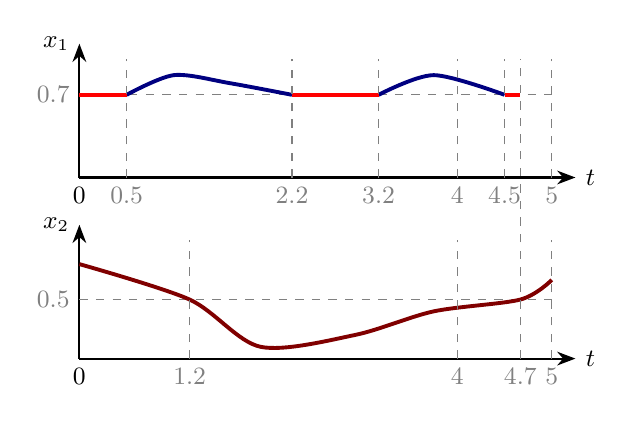
\begin{tikzpicture}[font=\small]
                    \centering
                    \begin{scope}
                        \draw[-Stealth, thick] (0,0) -- (6.3,0) node[right] {$t$};     
                        \draw[-Stealth, thick] (0,0) -- (0,1.7) node[above,left] {$x_1$};
                        \draw[dashed, color = gray] (0,1.05) node[left] {\black{$0.7$}} -- (6,1.05);
                        
                        \draw[color=NavyBlue, line width = 1.4pt, smooth, tension = 0.5] plot coordinates {
                            %(0, 0.75)
                            (0.6, 1.05)
                            (1.2, 1.3)
                            (1.9, 1.2)
                            (2.7, 1.05)};
                            %(3.3, 0.94)
                        \draw[color=NavyBlue, line width = 1.4pt, smooth, tension = 0.5] plot coordinates {
                            (3.8, 1.05)
                            (4.5, 1.3)
                            (5.4, 1.05)
                            %(6.0, 0.8)
                        };
                        \draw[color=red, line width = 1.6pt] plot coordinates{(0,1.05) (0.6,1.05)};
                        \draw[color=red, line width = 1.6pt] plot coordinates{(2.7,1.05) (3.8,1.05)};
                        \draw[color=red, line width = 1.6pt] plot coordinates{(5.4,1.05) (5.6,1.05)};
                        
                        \node at (0,0) [below] {\green{$0$}};
                        \draw[dashed, color = gray] (0.6, 0) node[below] {\orange{$0.5$}} -- (0.6,1.5);
                        \draw[dashed, color = gray] (2.7, 0) node[below] {\orange{$2.2$}} -- (2.7,1.5);
                        \draw[dashed, color = gray] (3.8, 0) node[below] {\orange{$3.2$}} -- (3.8,1.5);
                        \draw[dashed, color = gray] (4.8, 0) node[below] {\green{$4$}} -- (4.8,1.5);
                        \draw[dashed, color = gray] (5.4, 0) node[below] {\orange{$4.5$}} -- (5.4,1.5);
                        \draw[dashed, color = gray] (6,0) node[below] {\green{$5$}} -- (6,1.5);
                    \end{scope}

                    \begin{scope}[shift = {(0,-2.3)}]
                        \draw[-Stealth, thick] (0,0) -- (6.3,0) node[right] {$t$};     
                        \draw[-Stealth, thick] (0,0) -- (0,1.7) node[above,left] {$x_2$};
                        \draw[dashed, color = gray] (0,0.75) node[left] {\black{$0.5$}} -- (6,0.75);

                        \draw[color=Maroon, line width = 1.4pt, smooth, tension = 0.5] plot coordinates {
                            (0, 1.2)
                            (1.4, 0.75)
                            (2.3, 0.15)
                            (3.5, 0.3)
                            (4.5, 0.6)
                            (5.6, 0.75)
                            (6.0, 1)
                        };

                        \node at (0,0) [below] {\green{$0$}};
                        \draw[dashed, color = gray] (1.4, 0) node[below] {\orange{$1.2$}} -- (1.4,1.5);
                        \draw[dashed, color = gray] (4.8, 0) node[below] {\green{$4$}} -- (4.8,1.5);
                        \draw[dashed, color = gray] (5.6, 0) node[below] {\orange{$4.7$}} -- (5.6,3.8);
                        \draw[dashed, color = gray] (6,0) node[below] {\green{$5$}} -- (6,1.5);
                    \end{scope}
                     
                \end{tikzpicture}
                \end{adjustbox}
                \vspace{-4mm}
                \caption{Enforced Signal in \cref{exp:alg2}}
                \label{fig:after-enforce}
            \end{minipage}
        \end{figure*}
        
    %\hscomment{What about we change line \ref{al2line:3} to $(t,a)\gets$ event emitted by \cref{alg:signal-encoding}}
% \hscomment{Modified this to online one}
    \begin{algorithm}[H]
        %\caption{Algorithm Enforcer $E_\varphi(\automaton_\varphi,\tword,\signal$) }
        \caption{Algorithm Enforcer $E_\varphi(\signal$) }
        \label{algorithm} %\scriptsize
        \begin{algorithmic}[1]
            % \State $T \leftarrow 0$
            % \State $ currState \leftarrow  [l_0 , c:=0]$
            % \While {true}
            %     \For{$(\delta, a) \in \tword$ in buffer}
            %         \State $currState[1] = currState[1]+\delta$
            %         \State \footnotesize $currState[0], \signal'=\delta_{\automaton_{f}}(currState[0],  G(C), a, reset(C))$
            %         \State $release(\signal')$
            %     \EndFor		
            % \EndWhile
            % \State $T \leftarrow T +1$
            \State $\automaton_\varphi \gets $ TT constructed from $\varphi$ \label{al2line:0}
            \State $ \texttt{currState} \leftarrow  [l_0 , c:=0]$\label{al2line:1}
            \While {$true$}\label{al2line:2}
                %\State $(t, a)\gets \textsf{await\_event()}$ 
                \State $(t, a)\gets$ event emitted by \cref{alg:signal-encoding}\label{al2line:3}
                %\State $currState[0], output=\delta_{\automaton_{f}}(currState[0],  G(C), a, reset(C))$
                \State $\texttt{currState}, ~b =\textsf{make\_transition}_{\automaton_{\varphi}}(\texttt{currState}, t, a)$\label{al2line:4}
                \If{$b \neq\top$}
                    \State $\signal(t)=\textsf{Modify}(\signal(t),a,b, \varphi)$\label{al2line:6}
                \EndIf
                \State release $\signal$
            \EndWhile
        \end{algorithmic}
    \end{algorithm}


    % \begin{algorithm}[H]
    %     \caption{Algorithm Enforcer $E_f(\automaton_{f}, \tword, \signal$) }
    %     \begin{algorithmic}[1]
    %     \State $ currState \leftarrow  [l_0 , c:=0]$
    %         \While {true}
    %             \State (t, a) $\gets$ await event()
    %             \State $currState[0], output=\delta_{\automaton_{f}}(currState[0],  G(C), a, reset(C))$
    %             \If{output $\neq $$ \top$}
    %                 %\State $\signal'(t)=reconstruct(\signal(t), output, f)$
    %                 \State Pred=$pd(f)$	%\comment{Pred is the set of predicates in the STL formula f.}
    %     	        \State p=Pred[output]	%\comment{predicate at the specified index output within Pred.}
    %     	        \State $\signal(t)=minimize \mid \mid \signal(t)-y \mid \mid \text{ subject to }p(y)=True$
    %             \EndIf
    %             \State release($\signal$)
    %         \EndWhile
    %     \end{algorithmic}
    % \end{algorithm}




  \begin{example}[Enforcement of STL formula on a timed word]\label{exp:alg2}
      %We consider the STL formula $(\signal_1\ge 0.7)\until_{[4,5]}(\signal_2\ge 0.5)$, with $p_1\equiv \signal_1\ge 0.7$, $p_2\equiv \signal_2 \ge 0.5$ and signals $\signal_1$ and $\signal_2$ from Figure \ref{fig:signal-encoding}. 
      Continuing to \cref{exp:relavant-point}, recall that the STL property is defined as $p_1\until_{[4,5]} p_2$, where $p_1\equiv x_1\ge 0.7$, $p_2\equiv x_2 \ge 0.5$. %The TT of formula $\varphi = p_1\until_$ The time word is shown in \cref{fig:signal-encoding}.
      %The final timed word encoded from the signals (and the STL specification) is: $(\neg p_1 \land p_2, 0), (p_1 \land p_2, 0.5), (p_1 \land \neg p_2, 1.2), (\neg p_1 \land \neg p_2, 2.2), (p_1 \land \neg p_2, 3.2), (p_1 \land \neg p_2, 4),(\neg p_1 \land \neg p_2, 4.5), (\neg p_1 \land p_2, 4.7) \text{ and } (\neg p_1 \land p_2, 5)$. 
      \cref{tab:table_enf} gives the steps of enforcement of the timed word using Until Transducer. The signal at time points \{0, 2.2, 4.5, 4.7\} are modified to satisfy the STL formula. The modified signal is shown in \cref{fig:after-enforce}.
    \qedT
    \end{example}
%\spcomment{Reg Algo 2, how do you argue that the final output signal is sound with respect to the given STL formula? State changes are made upon the input. And after the state change Modify is called. Is it guaranteed that your Modify approach preserves the state?}

    The following theorem states the correctness of the enforcer described in \cref{algorithm}
    \begin{theorem}
        Given an STL formula $\varphi$ and a signal $\signal$, the enforcer $E_\varphi$ in \cref{algorithm} can enforce $\signal$ to satisfy $\varphi$, while ensuring that the \emph{soundness}, \emph{transparency}, and \emph{minimal modification} conditions in \cref{def:enforcer} are met. 
    \end{theorem}
    \begin{proof}
    The transparency of the enforcer is a direct result of \cref{propo1}, \cref{propo2}, and \cref{prop:composition}, as \cref{algorithm} will not modify the signal under the $\top$ output of the TT. The soundness of the enforcer is ensured by observing the truth that, the $\bot_p$ outputs of TT essentially indicate how to modify the input action to those inputs that can lead to a $\top$ output. The minimal modification condition is ensured by \cref{prop:modify}.
    \end{proof}
 % \hscommentinline{Here we may need a theorem to show our enforcer truly solve the problem in \cref{sec:Preliminaries and notations}}

  %\nzcomment{Yes, I agree. In addition, we also need to have a complexity analysis of our approach.}

    \paragraph{Complexity Analysis} The time complexity of \cref{algorithm} is multifaceted. The time complexity of the function $\textsf{make\_transition}_{\automaton{\varphi}}$ is $\mathcal{O}(m \times n)$, where $m$ is the number of states in the TT and $n$ is the size of the input alphabet. The time complexity of the function $\textsf{Modify}$ depends on the structure of the predicate function in the STL formula; it will be polynomial in the number of decision variables when the predicate functions are linear \cite{nesterov1994interior}.

    Other procedures, such as constructing the TT from the STL formula in \cref{sec: Transform STL into TA} (polynomial in the size of the TT, primarily influenced by the composition operator), and computing the values of the signal leading to the variable points in \cref{sec: Signal Encoding} (achieving quadratic convergence with the Newton-Raphson method), may be time-consuming. However, both procedures can be performed \emph{offline}, thus they do not impact the efficiency of our runtime enforcement algorithm.
\section{Case Study}
\label{Case Study}
We developed a prototype of our runtime enforcement algorithm in Python and applied this prototype to case studies on Autonomous Vehicles (AVs) to demonstrate the efficiency and scalability of our method. Three cases were considered in the experiments. The first case addresses the property of `safe stopping of AVs', the second focuses on `safe charging of AVs', while the third focuses on `safe deceleration of AVs'. All the cases underscore the efficiency (\cref{sec:efficiency}) and scalability (\cref{sec:scala}) of our method.

%In this section, we present a case study of an Autonomous Vehicle (AV)- a self-driving car. 
%AVs operate in dynamic environments, and ensuring precise control over critical signals is essential for safety and reliability. Due to environmental noise, sometimes, the critical signals can deviate from expected behaviour, potentially compromising safety.
%To address this, one can leverage formal runtime enforcement monitors that observe these signals as the vehicle operates. By specifying formal properties for each signal, the monitor can verify whether these properties hold at every moment. If a property is violated, the monitor can immediately correct the signal, ensuring the AV continues to perform safely. %This type of runtime enforcement is particularly useful in scenarios involving speed control, where strict limits are needed for example for safe stopping.\\

%include a formulate safety properties and demonstrate the enforcement. We provide empirical evidence that our approach is scalable.

\subsection{Efficiency Evaluation}\label{sec:efficiency}

    \paragraph{Safe stopping of AVs}
    Consider a scenario in which an AV is required to decelerate to a complete stop when approaching a red light or a designated stop point. This requirement is expressed by the property \((v \le 30)\until_{[5,10]} (v=0)\). This stipulates that \textit{the speed of the vehicle must ultimately reach $0$ within a time frame of $5$ to $10$ seconds, while maintaining a speed no larger than $30$ until then}.

    \begin{figure}[h]
        \centering
        \includegraphics[width=.76\linewidth,trim={18cm 0cm 0cm 0cm}, clip]{figures/speed.png}
        \caption{Enforcement of Speed Signal against Safe Stopping Property}
        \label{fig:speed}
    \end{figure}

    The results of our experiment are depicted in \cref{fig:speed}, where the blue signal represents the output after enforcement, while the orange one is the original signal. These results demonstrate that the enforcement monitor effectively adjusted the signal to ensure compliance with the STL property, while maintaining transparency and minimal modification. Specifically, the enforcer precisely addressed the four instances where the speed exceeded $30$ (sudden speed spikes), applying only the necessary changes without superfluous adjustments to the signal.
  
    \paragraph{Safe charging of AVs}
    Consider a scenario in the battery charging systems of AVs. Normally, the current stays within a safe range throughout a specified interval. If, however, the voltage reaches a specific volts, the system switches to a charging mode designed to safely handle higher currents. This condition is formally represented by the property \((V=4.2) \release_{[2,10]} (I<10)\), which indicates that \textit{the current will not exceed $10$ within a timeframe of $2$ to $10$ seconds, unless the voltage reaches $4.2$ volts earlier}.

    \begin{figure}[t]
        \centering
        \includegraphics[width=.76\linewidth, trim={0cm 0cm 18cm 0cm}, clip]{figures/battery_corrected.png}
        \includegraphics[width=.76\linewidth, trim={17.6cm 0cm 0cm 0cm}, clip]{figures/battery_corrected.png}
        %\vspace{-2mm}
        \caption{Enforcement of Voltage and Current Signals against Safe Charge Property}
        \label{fig:battery}
    \end{figure}

    The results of our experiment are depicted in \cref{fig:battery}, where the blue signal represents the output after enforcement, and the orange signal is the original one. These results illustrate that during the interval from $2$ to $10$ seconds, the current $I$ is minimally adjusted to remain below $10$, provided that the voltage $V$ does not reach $4.2$ volts.


    \paragraph{Safe deceleration of AVs}
    Consider a scenario of coordinated deceleration for stability and safety in AVs, where both wheels and motor controls slow down together, helping avoid sudden stops or imbalances. It is a dual-redundant safety feature: The wheel subsystem must ensure that its value does not exceed 30 within the timeframe and ultimately reaches zero between 5 and 10 seconds. Simultaneously, the motor control subsystem has the same requirement. This condition is formally represented by the property $(w \leq 30)\until_{[5,10]} (w = 0) \land (m \leq 30)\until_{[5,10]} (m = 0)$, which indicates that \textit{both the wheels and motor control must ultimately reach $0$ within a time frame of $5$ to $10$ seconds while maintaining the values no larger than $30$ until then}.
    % \hscomment{@Saumya. The size of figure for the third experiment seems different from the other two, could you make the size the same?}
    \begin{figure}[t]
        \centering
        \includegraphics[width=0.83\linewidth, trim={0cm 0.5cm 0cm 0.9cm}, clip]{figures/wheel.png}
        \includegraphics[width=0.83\linewidth, trim={0cm 0.5cm 0cm 0.6cm}, clip]{figures/motor.png}
        %\vspace{-2mm}
        \caption{Enforcement of Wheel and Motor Control Signals against Safe Deceleration Property}
        \label{fig:wheel_motor}
    \end{figure}

    The results of our experiment are depicted in \cref{fig:wheel_motor}. These results illustrate that during the interval from $5$ to $10$ seconds, the wheel ($w$) and motor control ($m$) are minimally adjusted to remain below $30$, provided that these signals do not reach $0$ volts.
    
    
\subsection{Scalability Evaluation}\label{sec:scala}
    %\hscomment{The experimental results appear efficient; however, incorporating STL properties that include Boolean operators $\land$ or $\lor$ could enhance our result.}
    To assess the scalability of our approach, we conducted experiments in which we progressively increased the complexity of the signal - specifically, the number of violation points in the signal - to examine how enforcement time is affected. The results, presented in \cref{tab:performance} for the three scenarios mentioned earlier, show that the enforcement time (measured in milliseconds) increases in a piecewise linear fashion as the number of violations grows. This behavior is consistent with the predictions of our complexity analysis.
    % \hscomment{I changed the capital of the table from STL formula to the specific property name, please check which type is better.}
    \begin{table*}[t]
        \centering
            \captionsetup{font={small}}
            \caption{Experimental results with varying violation points in the signal}
            \vspace{-0.32cm}
            \label{tab:performance}
            \begin{center}
                % \begin{tabular}{c c ccc c ccc} 
                %     \toprule
                %     \multirow{2}{*}{$\#v$} &~& \multicolumn{3}{c}{$(v \leq 30)\until_{[5,10]} (v = 0)$} &~& \multicolumn{3}{c}{$(V=4.2) \release_{[2,10]} (I<10)$}\\
                %     \cmidrule{3-5}\cmidrule{7-9}
                %     && $\textsf{len}(\tword)$ &~& \textsf{time}(ms) &~& $\textsf{len}(\tword)$ &~& \textsf{time}(ms)\\
                %     \midrule
                %     2 &~& 6 &~& 0.117 &~& 5 &~& 0.086\\
                %     4 &~& 8 &~& 0.124 &~& 7 &~& 0.146\\
                %     6 &~& 10 &~& 0.14 &~& 9 &~& 0.156\\
                %     8 &~& 12 &~& 0.156 &~& 11 &~& 0.173\\
                %     10 &~& 14 &~& 0.186 &~& 13 &~& 0.19\\
                %     12 &~& 14 &~& 0.202 &~& 15 &~& 0.199\\
                %     14 &~& 18 &~& 0.237 &~& 14 &~& 0.215\\
                %     16 &~& 16 &~& 0.217 &~& 17 &~& 0.262\\
                %     18 &~& 19 &~& 0.237 &~& 19 &~& 0.265\\
                %     20 &~& 22 &~& 0.287 &~& 17 &~& 0.242\\
                %     \bottomrule
                % \end{tabular}
                \begin{tabular}{@{}ccccccccc@{}}
                    \toprule
                    %\multirow{2}{*}{$\#v$} & \multicolumn{2}{c}{$(v \leq 30)\until_{[5,10]} (v = 0)$} &~& \multicolumn{2}{c}{$(V=4.2) \release_{[2,10]} (I<10)$} &~& \multicolumn{2}{c}{$(w \leq 30)\until_{[5,10]} (w = 0) \land (m \leq 30)\until_{[5,10]} (m = 0)$} \\
                    \multirow{2}{*}{$\#v$} & \multicolumn{2}{c}{\textit{Safe stopping of AVs}} &~& \multicolumn{2}{c}{\textit{Safe charging of AVs}} &~& \multicolumn{2}{c}{\textit{Safe deceleration of AVs}} \\
                    \cmidrule{2-3} \cmidrule{5-6} \cmidrule{8-9}
                                       & $\textsf{len}(\tword)$        & \textsf{time}(ms)       &~& $\textsf{len}(\tword)$        & \textsf{time}(ms)         &~& $\textsf{len}(\tword)$        & \textsf{time}(ms)          \\ \midrule
                    2                  & 6        & 0.117     &~& 5        & 0.086      &~& 9        & 0.221      \\ 
                    4                  & 8        & 0.124     &~& 7        & 0.146      &~& 13       & 0.369      \\ 
                    6                  & 10       & 0.14      &~& 9        & 0.156      &~& 17       & 0.419      \\ 
                    8                  & 12       & 0.156     &~& 11       & 0.173      &~& 20       & 0.629      \\ 
                    10                 & 14       & 0.186     &~& 13       & 0.19       &~& 21       & 0.631      \\ 
                    12                 & 14       & 0.202     &~& 15       & 0.199      &~& 26       & 0.719      \\ 
                    14                 & 18       & 0.237     &~& 14       & 0.215      &~& 27       & 0.8        \\ 
                    16                 & 16       & 0.217     &~& 17       & 0.262      &~& 28       & 0.867      \\ 
                    18                 & 19       & 0.237     &~& 19       & 0.265      &~& 35       & 0.916      \\ 
                    20                 & 22       & 0.287     &~& 17       & 0.242      &~& 30       & 0.988      \\ \bottomrule
                    \end{tabular}
            \end{center}
            %\vspace*{-\baselineskip}
            %\vspace*{1mm}
            \small{ 
                $\textsf{len}(\tword)$: the length of time word encoded from the signal;~
                $\#v$: the number of violation points in signal
            } 
        \end{table*}

        Overall, our method demonstrates robust capabilities in runtime enforcement for signals against properties specified using STL. It ensures compliance with requirements for soundness, transparency, and minimal modification across all scenarios. Moreover, it exhibits high effectiveness in managing complex signals, indicating that the time required is minimal. %Therefore, our approach represents a high-performance method for achieving runtime enforcement.
        
% \subsection{Safe AV stopping}
% \noindent \textit{Scenario Description and Example Property: }
%     Consider a scenario where an AV must decelerate to a complete stop when approaching a red light or a designated stopping point. We specify property number (1) of Example \ref{example:Properties in STL} saying that: \textit{The value of the speed signal will be 0 between 5 to 10 seconds; until then the value of the signal is less than 30}, i.e., 
%     \begin{align*}
%         (\signal  < 30) \until_{[5,10]} (\signal = 0)
%     \end{align*}
%     %\noindent \textit{Need of Runtime Enforcement}
%     % Above specified property can be enforced on the vehicle’s speed, such that it remains below a certain threshold while it approaches the stop and comes to a complete halt within a defined time window. By enforcing this speed constraint, the AV can stop smoothly and safely at designated locations, reducing safety risks. Such a predictable stopping behaviour is essential for AVs, especially in urban settings where other road users might be around. This case study describes the above property and its enforcement process in an AV context.


%     %\noindent \textit{Generating Test Signals with Violations: } %When generating test speed signals for the AV speed, it is essential to mimic realistic behavior under conditions where the vehicle may partially deviate from specified STL constraints. A detailed approach for generating these test speed signals, ensuring they exhibit both compliance and controlled violations for effective runtime enforcement is given below:\\
%     %
%     %\noindent \textit{Setting Initial Parameters for Speed Signal Generation}:
%     %The initial speed of the vehicle at $t=0$ is set to 30. %This creates a realistic starting condition where the vehicle's speed is initially within the safe range but may approach the violation threshold as it evolves.\\
%     %\noindent \textit{Decaying Speed signal}:
%     %To model deceleration i.e., the vehicle slowing down as it approaches a red light or stop, we used a linear decay function (where the rate of deceleration is constant) to ensure that the speed goes towards 0 by $t=10$ seconds.  
%     %\noindent \textit{Adding Noise/ Controlled Violations}:
%     %To test the enforcement monitor to detect and correct violations, we added speed spikes at some random time points to create a temporary violation of $\signal<30$.
%     %
%     \begin{figure*}%[H]
%         \centering
%         \includegraphics[width=1\linewidth]{figures/speed.png}
%         \caption{Generated vs Corrected Speed signal}
%         \label{fig:speed}
%     % \end{figure*}
%     % \begin{figure*}%[htp]
%     %     \centering
%         \includegraphics[width=0.9\linewidth]{figures/battery_uncorrected.png}
%         \includegraphics[width=0.9\linewidth]{figures/battery_corrected.png}
%         \caption{Generated vs Corrected V and I signals}
%         \label{fig:battery}
%     \end{figure*}
    
%     \noindent \textit{Encoding and correcting the signals: } The original signal is given in the left plot in Figure \ref{fig:speed}. 
%     Following Section \ref{sec: Signal Encoding}, we encode the signal into a timed word, needed for enforcement. This involves recording the truth value of predicates of the STL formula at both variable points and relevant points within the signal.
%     %
%     The encoded time word $\tword$ is as follows: % [[0.0, 'a', '$not\_b$'], [5.0, 'a', '$not\_b$'], [5.1, '$not\_a$', '$not\_b$'], [5.2, 'a', '$not\_b$'], [6.3, '$not\_a$', '$not\_b$'], [6.4, 'a', '$not\_b$'], [9.7, 'a', 'b'], [10.0, 'a', 'b']] 
%     [[0.0, 'a', 'not\_b'], [0.5, 'not\_a', 'not\_b'], [0.6, 'a', 'not\_b'], [2.2, 'not\_a', 'not\_b'], [2.3, 'a', 'not\_b'], [2.8, 'not\_a', 'not\_b'], [2.9, 'a', 'not\_b'], [5.0, 'a', 'not\_b'], [9.6, 'a', 'b'], [10.0, 'a', 'b']],
%     where $a$ means $\signal< 30$ is satisfied, $not\_a$ means  $\signal< 30$ is not satisfied, $b$ means $\signal= 0$ is satisfied and $not\_b$ means  $\signal = 0$ is not satisfied by the generated speed signal. 

%     %\noindent \textit{Correcting signals: } %\subsubsection{Timed Transducer for the Until Operator}: 
%     Following Section \ref{sec: Transform STL into TA}, we construct a timed transducer model for the until operator of STL, where $p_1 \equiv \signal<30$ and $p_2 \equiv \signal=0$. %In case, the signal needs to be corrected, the transducer outputs the minimal value of the signal by which the signal is to be corrected, in the implementation.
%     Following Algorithm \ref{algorithm}, we construct the enforcer here.  
%     %
%     %\subsection{Results}
%      The enforcement monitor corrected the signal to ensure compliance with the STL property as seen in the right plot in Figure \ref{fig:speed}. The enforcer accurately corrected the three violations without unnecessary corrections to the signal.

%     \subsection{Safe battery charging of AV}
%     \noindent \textit{Scenario Description and Example Property: } Consider a scenario in battery charging systems in AVs that under normal conditions, the current remains within a safe range (below 10 amps) during a specified interval. However, if the voltage reaches 4.2 volts within this time frame, the system can recognize this as a signal to relax the current limit footnote{The voltage condition (4.2 volts) could indicate a specific state, such as a change in the charging mode, where it is safe to allow higher currents}. To ensure such safe operating conditions, one can define the following STL property:
%     \begin{align*}
%         (V==4.2) \release_{[2,10]} (I<10)
%     \end{align*}  
%     %and monitor this property in real time. Such monitoring is essential in applications like electric vehicles or electronic devices, where excessive current could lead to overheating or damage, making strict limits crucial for system safety and longevity.

%     \noindent \textit{Encoding and correcting the Signal: } The original generated signals of $V$ and $I$ are given in the top plots in Figure \ref{fig:battery}. The corresponding corrected signals are given in the bottom plots in Figure \ref{fig:battery}, where we observe that, during the interval from 2 to 10 seconds, the current $I$ is minimally adjusted to stay below 10 as long as the voltage $V$ is not equal to 4.2.
%     % \begin{figure*}[htp]
%     %     \centering
%     %     \includegraphics[width=0.9\linewidth]{figures/battery_uncorrected.png}
%     %     \includegraphics[width=0.9\linewidth]{figures/battery_corrected.png}
%     %     \caption{Generated vs Corrected V and I signals}
%     %     \label{fig:battery}
%     % \end{figure*}


% The enforcer, transducer and signal processing are all implemented in Python. 



%     \subsection{Evaluating Performances}
% To evaluate the performance of our approach to see its scalability, we conducted experiments where we linearly increased the number of violations in the signals to observe how the enforcement time changes. %Specifically, we examined whether a linear increase in violations results in a linear increase in enforcement time. 
% %These experiments were conducted with different signals and different STL formulas.
% The results, displayed in Table \ref{Tab:performance} for the above scenarios, indicate that the enforcement time (measured in ms) increases (piecewise) linearly with a linear increase in the number of violations.





% \begin{table}[]
% \begin{tabular}{@{}|l|ll|ll|@{}}
% \toprule
% \multicolumn{1}{|c|}{\multirow{2}{*}{$\#v$}} & \multicolumn{2}{c|}{$(x \leq 30)\until_{[5,10]} (x = 0)$} & \multicolumn{2}{c|}{$(x_1=4.2)\release_{[2,10]}(x_2<10)$}     \\ \cmidrule(l){2-5} 
% \multicolumn{1}{|c|}{}                   & \multicolumn{1}{c|}{$len(\sigma)$} & \multicolumn{1}{c|}{T(ms)} & \multicolumn{1}{c|}{$len(\sigma)$} & \multicolumn{1}{c|}{$T(ms)$} \\ \midrule
% 2                                        & \multicolumn{1}{l|}{6}          & 0.117                      & \multicolumn{1}{l|}{5}          & 0.086                      \\ \midrule
% 4                                        & \multicolumn{1}{l|}{8}          & 0.124                      & \multicolumn{1}{l|}{7}          & 0.146                      \\ \midrule
% 6                                        & \multicolumn{1}{l|}{10}         & 0.14                       & \multicolumn{1}{l|}{9}          & 0.156                      \\ \midrule
% 8                                        & \multicolumn{1}{l|}{12}         & 0.156                      & \multicolumn{1}{l|}{11}         & 0.173                      \\ \midrule
% 10                                       & \multicolumn{1}{l|}{14}         & 0.186                      & \multicolumn{1}{l|}{13}         & 0.19                       \\ \midrule
% 12                                       & \multicolumn{1}{l|}{14}         & 0.202                      & \multicolumn{1}{l|}{15}         & 0.199                      \\ \midrule
% 14                                       & \multicolumn{1}{l|}{18}         & 0.237                      & \multicolumn{1}{l|}{14}         & 0.215                      \\ \midrule
% 16                                       & \multicolumn{1}{l|}{16}         & 0.217                      & \multicolumn{1}{l|}{17}         & 0.262                      \\ \midrule
% 18                                       & \multicolumn{1}{l|}{19}         & 0.237                      & \multicolumn{1}{l|}{19}         & 0.265                      \\ \midrule
% 20                                       & \multicolumn{1}{l|}{22}         & 0.287                      & \multicolumn{1}{l|}{17}         & 0.242                      \\ \bottomrule
% \end{tabular}
% \caption{Effect on time taken ($T(ms)$) by enforcement by varying the number of violations ($v$).}
% \label{Tab:performance}
% \end{table}


% \subsection{Discussion}
% This experimental analysis is conducted offline. We assume the entire signal is available to us upfront, allowing us to extract all significant variables and relevant points, construct an input word, and then perform enforcement on each event one by one. However, an alternative approach could involve processing the signal in real-time, constructing timed events at runtime as the signal arrives, and enforcing properties accordingly.



% \subsubsection{Timed Transducer Model of Until Operator}
%  \begin{figure*}[H]
%      \centering
%      \includegraphics[width=1\linewidth]{figures/speed_corrected.png}
%      \caption{Enforcing speed constraint}
%      % \label{fig:enter-label}
%  \end{figure*}




%\section{Main Results}
\label{sec:results}
We now state the soundness and completeness of the translation of the STL formulas into the transducers.

We propose here the equivalence of the Until and Release operator of STL and its transducer. %A similar proof is done for the Release operator of STL and its transducer.
%\hscomment{The notation we use should be align with that in \cref{sec: Transform STL into TA}. $\varphi_1\until_I\varphi_2$ should be $p_1\until p_2$.}

\begin{proposition}[Equivalence of Until operator of STL and its transducer]    
\label{propo1}
        Let $\signal$ be the signals. Let $\tword$ be its encoded timed word for the given STL formula $p_1\until_{[t_1,t_2]}p_2$. %Let $\rho$ be the run of $\automaton_{p_1\until_{[t_1,t_2]}p_2}$ over $\sigma$ from its initial state. 
        Let $\bm{\omega}_{\top}$ be the output timed word for the accepting run over $\tword$, where the output of all transition being $\top$. Then,

        
        %If the encoded timed word is accepted by the transducer of Until operator $\automaton_{p_1\until_{[t_1,t_2]}p_2}$, and the output of  all the transitions for that accepting run,  is $\top$ then the corresponding signals  $\signal$  satisfy $ p_1\until_{[t_1,t_2]}p_2$, i.e.,
        %\hscomment{We have not define the notion $\mathcal{L}(\automaton)$. Please refer to \cref{sec:Preliminaries and notations} for the notation of $\bm{\omega} = \llangle\automaton\rrangle(\tword)$ in line 240-244, I defined this notation specifically for writing the proposition.}
        % \begin{align*}
        %     %\sigma \in \mathcal{L}(\automaton_{p_1\until_{[t_1,t_2]}p_2})  \land \forall \delta \in \rho, \lambda(\delta)=\top \implies \signal \models p_1\until_{[t_1,t_2]}p_2
        %     \llangle\automaton_{p_1\until_{[t_1,t_2]}p_2}\rrangle(\tword) \land \forall \delta \in \rho, \lambda(\delta)=\top \implies \signal \models p_1\until_{[t_1,t_2]}p_2
        % \end{align*}
        % \hscomment{Is this version more clear?}
        % \saucomment{yes. only thing is that: we cant use $SignEncode$ because SignEncode gives timed event at time t and not the entire encoded-word for the $\signal$}
        % \hscomment{okay, this version is more suitable.}
        %Let \(\signal\) be the signal and \(\tword = \textsf{SignEncode}(p_1 \until_I p_2, \signal)\). Let $\bm{\omega}_{\top}$ denote the timed word where the action of all its events is $\top$. Then,
        \[
            \llangle\automaton_{\until}\rrangle(\tword) = \bm{\omega}_{\top} \iff \signal \models p_1 \until_{[t_1, t_2]} p_2
        \]
        
\end{proposition}

\begin{proposition}[Equivalence of Release operator of STL and its transducer]   
\label{propo2}
    Let $\signal$ be the signals. Let $\tword$ be its encoded timed word for the given STL formula $p_1\release_{[t_1,t_2]}p_2$. %Let $\rho$ be the run of $\automaton_{p_1\release_{[t_1,t_2]}p_2}$ over $\sigma$ from its initial state. 
    Let $\bm{\omega}_{\top}$ be the output timed word for the accepting run over $\tword$, where the output of all transitions being $\top$. Then,
        
        %If the encoded timed word is accepted by the transducer of Until operator $\automaton_{p_1\release_{[t_1,t_2]}p_2}$, and the output of  all the transitions for that accepting run,  is $\top$ then the corresponding signals  $\signal$  satisfy $ p_1\release_{[t_1,t_2]}p_2$, i.e.,

        \begin{align*}
        \llangle\automaton_{\release}\rrangle(\tword) = \bm{\omega}_{\top} \implies \signal \models p_1 \release_{[t_1, t_2]} p_2
        %\sigma \in \mathcal{L}(\automaton_{p_1\release_{[t_1,t_2]}p_2})  \land \forall \delta \in \rho, \lambda(\delta)=\top \implies \signal \models p_1\until_{[t_1,t_2]}p_2
        \end{align*}
\end{proposition}

%%%%%%%%%%%%%%%%%%%%%%%%%%%%%%%%%%%%%%%%%%%%%


% \begin{proposition} 
% \label{propo3}
%     Let $\signal$ be the signals and let $\tword$ be the corresponding encoded timed word. If signals  satisfy the Until formula $ p_1\until_{[t_1,t_2]}p_2$, then its encoded word is accepted by its transducer, i.e., 
%     \begin{align*}
%         \signal \models p_1\until_{[t_1,t_2]}p_2 \implies \llangle\automaton_{\until}\rrangle(\tword) \red{=\bm{\omega}_{\top}} %\sigma \in \mathcal{L}(\automaton_{p_1\until_{[t_1,t_2]}p_2}) 
%     \end{align*}
% \end{proposition}

% \begin{proposition} 
% \label{propo4}
%     Let $\signal$ be the signals and let $\tword$ be the corresponding encoded timed word. If signals  satisfy the Release formula $ p_1\release_{[t_1,t_2]}p_2$, then its encoded word is accepted by its transducer, i.e., 
%     \begin{align*}
%         \signal \models p_1\release_{[t_1,t_2]}p_2 \implies \llangle\automaton_{\until}\rrangle(\tword) %\tword \in \mathcal{L}(\automaton_{p_1\release_{[t_1,t_2]}p_2}) 
%     \end{align*}
% \end{proposition}

The proofs of the propositions are provided in Appendix \ref{sec:appendix}.
\section{Related Works}
\label{sec:RL}
% \hscommentinline{this section need to be rewrite.}
\paragraph{Runtime enforcement for reactive systems.}
A framework to synthesize enforcers for reactive systems, called shields, from a set of safety properties was introduced in \cite{10.1007/978-3-662-46681-0_51}. The uni-directional shield observes inputs from the environment and outputs from the system (program) and transforms erroneous outputs. It considered untimed properties expressed as automata. 

Authors in \cite{10.1145/3126500,10.1145/3092282.3092291,10.1109/TII.2019.2945520} extendes \cite{10.1007/978-3-662-46681-0_51} and considered bi-directional runtime enforcement for reactive systems. The enforcer presented a monitoring framework which monitors both the inputs and the outputs of a synchronous program and (minimally) edits erroneous inputs/outputs in order to guarantee a given property.  In \cite{10.1145/3092282.3092291,10.1109/TII.2019.2945520}, the properties are discrete properties, expressed using a variant of timed automata  %(dense time properties can be expressed as Timed Automata) 
called Discrete Timed Automata (DTA) and Valued Discrete Timed Automata (VDTA). These are TAs with integer-valued clocks (i.e., FSMs extended with a set of integer variables that are used as discrete clocks, for instance, to count the number of ticks before a certain event occurs).  The use of DTA/VDTA over TA is primarily motivated by the fact that the approach can directly use a formulation similar to synchronous languages, where time is discretized. This makes the overall algorithm simple and does not require region or zone graph construction. All transitions take one tick relative to the ticks of a synchronous global clock inspired by synchronous languages. The environmental inputs are captured %\sout{by an additional piece of hardware called the Reactive Functional Unit (RFU)} 
and are made available. % on the next tick boundary (at the onset of the next tick). 
During a tick, all three components – the environment, the program, and the enforcer- are executed once. 


The monitoring frameworks in \cite{10.1145/3092282.3092291,10.1109/TII.2019.2945520} are for discrete systems where they sampled the execution (i.e. the inputs signal occurring in the environment) to contain a number of observable state changes. For continuous timed systems, however, variables can change arbitrarily fast. For monitoring signals of time-continuous systems for dense-time properties using \cite{10.1145/3092282.3092291,10.1109/TII.2019.2945520}, the observations can be made only at discrete moments, each observation contains only partial information. This is not effective. Because only the whole set of possible observations of a particular execution can restore all information on that execution, thus, this work contributes an enforcement mechanism for dense-time real-valued signals for continuous timed systems. 

\paragraph{STL for specifying properties of CPS} STL \cite{10.1007/978-3-540-30206-3_12} is used for specifying linear-time properties of continuous real-valued signals. 
The logic of STL is based on a bounded subset of the real-time logic MITL \cite{10.1145/227595.227602} i.e. MITL$_{[a,b]}$. 
In MITL$_{[a,b]}$ all temporal modalities are restricted to intervals of the form $[a, b]$
with $0 \leq a < b$ and $a, b \in \mathbb{Q}_{\geq 0}$, where the behavior of a system is observed for a finite time interval. 

There exist frameworks for monitoring STL properties. For example, the framework in \cite{10.1007/978-3-540-30206-3_12} automatically creates property monitors that can check whether a given signal of bounded length and finite variability satisfies the property. However, this was for offline monitoring and not for correcting the signal if not according to the property. Authors in \cite{sun2024redriver} attempt enforcement (correcting a signal) specifically for the self-driving realm. %They essentially handle an offline runtime enforcement problem: 
It is based on the predictive environment constructed by the sensors of the car. If the AV is predicted to potentially violate them in the near future (based on the quantitative semantics of STL), the REDriver framework repairs the trajectories using a gradient-driven algorithm. However, in some situations, the enforcer may not have access to the prediction of future signals.


Our work presents a more general approach to enforcing STL properties. Unlike existing literature, it adopts a more formal enforcement method, where the enforcer corrects the signal while adhering to some critical constraints.


\vspace{-2mm}
\section{Conclusion}\label{sec:conclusion}
In this paper, we presented RecDreamer, a novel approach to mitigating the Multi-Face Janus problem in text-to-3D generation. Our solution introduces a rectification function to modify the prior distribution, ensuring that the resulting joint distribution achieves uniformity across poses. By expressing the modified data distribution as the product of the original density and the rectification function, we seamlessly integrate this adjustment into the score distillation algorithm. This allows us to derive a particle optimization framework for uniform score distillation. Additionally, we developed a pose classifier and implemented reliable approximations and simulations to enhance the particle optimization process. Extensive experiments on both 2D and 3D synthesis tasks demonstrate the effectiveness of our approach in addressing the Multi-Face Janus problem, resulting in more consistent geometries and textures across different views.

\textbf{Limitations.} While our method significantly reduces bias in prior distributions, further exploration of 3D modeling with multi-view priors could improve geometric and texture consistency. Extending our approach through deeper research into conditional control presents another promising avenue for addressing these challenges in future work. 
%%
%% The acknowledgments section is defined using the "acks" environment
%% (and NOT an unnumbered section). This ensures the proper
%% identification of the section in the article metadata, and the
%% consistent spelling of the heading.
% \begin{acks}
% To Robert, for the bagels and explaining CMYK and color spaces.
% \end{acks}

%%
%% The next two lines define the bibliography style to be used, and
%% the bibliography file.
\bibliographystyle{ACM-Reference-Format}
\bibliography{reference}


%%
%% If your work has an appendix, this is the place to put it.
%\newpage
\appendix

\section*{Appendix}

%We here provide the proofs of the Propositions.
\section{Proof of Propositions}\label{sec:appendix}

\restateUntil*
% It states that, for the signals $\signal$ if its encoded timed word $\tword$ is accepted by the transducer of Until operator $\automaton_{p_1\until_{[t_1,t_2]}p_2}$ and the output of  all the transitions for that accepting run, is $\top$, then the corresponding signals  $\signal$  satisfy $ p_1\until_{[t_1,t_2]}p_2$, and vice versa i.e.,
%             \[
%             \llangle\automaton_{\until}\rrangle(\tword) = \bm{\omega}_{\top} \iff \signal \models p_1 \until_{[t_1, t_2]} p_2
%             \]
            

    \begin{proof}To prove the above proposition, it suffices to demonstrate it in two steps/implications. Once both implications are established, it follows that the proposition holds. Thus, let us prove the proposition in 2 steps:

    \begin{tcolorbox}[boxrule=.5pt,colback=white,colframe=black!75]
    \[
        1.~~~~ \llangle\automaton_{\until}\rrangle(\tword) = \bm{\omega}_{\top} \implies \signal \models p_1 \until_{[t_1, t_2]} p_2
    \]
    \end{tcolorbox}
    
    Let us consider the following cases based on the events received in time intervals: $[0, t_1], (t_1,t_2]$.
    \begin{enumerate}
        \item Case 1: when the time interval is $[0,t_1]$:\\
        Based on the events received at $t\in [0,t_1]$, we have the following sub-cases:
        \begin{enumerate}
            \item Case 1a: $p_1$ is continuously received by the transducer at $t \in [0,t_1]$ with the output of all transitions being $\top$ and $p_2$ is received at $t\in[t_1,t_1]$ with the output of the transition being $\top$ again.

            The sequence of locations visited by the transducer for this case will be $l_0, l_1, l_2$. We see that the final location $l_2$ is reached by the transducer, thus $\llangle\automaton_{\until}\rrangle(\tword) = \bm{\omega}_{\top}$.

            According to the semantics of STL, if $p_2$ is received at $t\in[t_1, t_1]$ until that if $p_1$ is continuously received, then the STL formula is satisfied by the signal corresponding to $\tword$. Thus the proposition holds for this sub-case.
            
            \item Case 1b: $p_1$ is not true at $t \in [0,t_1]$ with the output of all transitions being $\bot_{p_1}$ and $p_2$ is true at $t\in[t_1,t_1]$.

            The proposition trivially holds here as well.\\
            
        \end{enumerate}
        \item Case 2: when the time interval is $(t_1,t_2]$:\\
         Based on the events received at $t\in (t_1,t_2]$, we have the following sub-cases:
        \begin{enumerate}
            \item Case 2a: $p_2$ is received by the transducer at $t \in (t_1,t_2]$ with the output of transition being $\top$  and $p_1$ is continuously received until that with the output of all transitions being $\top$.
            
            The sequence of locations visited by the transducer for this case will be $l_0, l_1, l_3, l_2$. We see that the final location $l_2$ is reached by the transducer, thus $\llangle\automaton_{\until}\rrangle(\tword) = \bm{\omega}_{\top}$.

            According to the semantics of STL, if $p_2$ is received at $t\in (t_1,t_2]$ until that $p_1$ is continuously received, then the STL formula is satisfied by the signal corresponding to $\tword$. Thus the proposition holds for this sub-case.

            \item Case 2b: $p_2$ is not true at $t\in(t_1,t_2]$ until that time $p_1$ is true, with the output of transition being $\bot_{p_2}$. The proposition trivially holds here as well.

            \item Case 2c: $p_2$ is true at $t\in(t_1,t_2]$ however until that time $p_1$ is not true, with the output of transition being $\bot_{p_1}$. The proposition trivially holds here as well.

            \item Case 2d: $p_2$ is not true at $t\in(t_1,t_2]$ however until that time $p_1$ is also not true, with the output of transition being $\bot_{p_1}$ or $\bot_{p_2}$ accordingly. The proposition trivially holds here as well. The proposition trivially holds here as well.
             
        \end{enumerate}
    \end{enumerate}


%%%%%%%%%%%%%%%%%%%%%%%%%%%%%%%%%%%%%%%%%%%%%%%%%%%%%
\begin{tcolorbox}[boxrule=.5pt,colback=white,colframe=black!75]
    \[
        2. ~~~~\signal \models p_1 \until_{[t_1, t_2]} p_2  \implies \llangle\automaton_{\until}\rrangle(\tword) = \bm{\omega}_{\top}
    \]
    \end{tcolorbox}



Let us consider the following cases based on the events received in time intervals: $[0, t_1], (t_1,t_2]$.
    \begin{enumerate}
        \item Case 1: when the time interval is $[0,t_1]$: an STL formula is satisfied at $t\in [0, t_1]$ by signal $\signal$, if $p_1$ of the encoded word $\tword$ of $\signal$ is continuously true and $p_2$ of the encoded word $\tword$ of $\signal$ is true at $t\in[t_1, t_1]$.

        For that encoded word $\tword$ of signal $\signal$, the transducer makes a sequence of transitions involving locations $l_0, l_1, l_2$ (with the output being $\top$ for all the transitions) and goes to the accepting state $l_2$. Thus,  $\llangle\automaton_{\until}\rrangle(\tword) = \bm{\omega}_{\top}$ and the proposition holds.

        \item  Case 2: when the time interval is $(t_1,t_2]$: an STL formula is satisfied at $t\in (t_1,t_2]$ by signal $\signal$, if $p_2$ of the encoded word $\tword$ of $\signal$ is received at $t\in (t_1,t_2]$ and  $p_1$ of the encoded word  $\tword$ of $\signal$  is continuously true until that.

        For that encoded word $\tword$ of signal $\signal$, the transducer makes a sequence of transitions involving locations $l_0, l_1, l_3, l_2$ (with the output being $\top$ for all the transitions) and goes to the accepting state $l_2$. Thus,  $\llangle\automaton_{\until}\rrangle(\tword) = \bm{\omega}_{\top}$ and the proposition holds.\\
    \end{enumerate}
\end{proof}

% \restateRelease*
% \begin{proof}
%     The proof is similar to that of \cref{propo1} and is omitted here.
% \end{proof}

\restateComposition*
\begin{proof}
    Let us prove this proposition using induction on the predicates. There will be two distinct cases based on $op\in \{\land, \lor\}$. Let us prove this proposition for $op= \{\land\}$. Similar proof will follow for $op= \{\lor\}$.\\
    
    \noindent \textit{Induction basis.} Consider STL formula $\varphi_1 \land \varphi_2$. Let us consider following cases:

    \begin{enumerate}
        \item Case 1: $\phi_1 \until_{[t_1, t_2]} \phi_2 \land \top$ \\
        where $\varphi_1 \equiv \phi_1 \until_{[t_1, t_2]} \phi_2$ and $\varphi_2 \equiv \top$.\\
        
        (Similar proof will follow for  $\top \land \phi_1 \until_{[t_1, t_2]} \phi_2$.)\\
        
        $\top$ (the true predicate) represents a property or a transducer that is always true, regardless of time constraints or inputs. A timed transducer for $\top$ would have only one state, an "accepting" state with a self-loop transition on this state allowing any input or no input to be processed at any time and $\top$ as output. 

        The structure (states and transitions) of $\land$-product of transducers $\automaton_{\phi_1 \until_{[t_1, t_2]} \phi_2}$ and $\automaton_{\top}$ will be the similar as transducer $\automaton_{\phi_1 \until_{[t_1, t_2]} \phi_2}$ (with $\top$ also an output for all transitions indicating predicate $\top$ is true).

        And from proposition \ref{propo1}, we will have following results:        
        $\llangle\automaton_{\phi_1 \until_{[t_1, t_2]} \phi_2} ~\times_{\land} ~\automaton_{\top}\rrangle(\tword) = \bm{\omega}_{\top} \iff \signal \models \phi_1 \until_{[t_1, t_2]} \phi_2 ~\land ~\top$.
        Thus, the proposition holds.
        
        \item Case 2: $p_1 \release_{[t_1, t_2]} p_2 \land \top$ \\
        (or similarly, $\top \land p_1 \release_{[t_1, t_2]} p_2$)\\

        Similar proof follows for this case as well.
    \end{enumerate}

    \noindent \textit{Induction Step.}
    \begin{enumerate}
        \item Case 1: $\phi_1 \until_{[t_1, t_2]} \phi_2 \land \phi_3 \until_{[t_3, t_4]} \phi_4$\\
        where $\varphi_1 \equiv \phi_1 \until_{[t_1, t_2]} \phi_2$ and $\varphi_2 \equiv \phi_3 \until_{[t_3, t_4]} \phi_4$.

        Let us consider sub-cases based on time intervals.
        \begin{enumerate}
            \item Case: when the time interval is $[0,t_1]$:
            \begin{enumerate}
                \item Case: $\phi_1$ and $\phi_3$ are continuously received by the transducer at $t \in [0,t_1]$ and  $t \in [0,t_3]$ respectively, with the output of all transitions being $\top$. $\phi_2$ and $\phi_4$ are received at $t\in[t_1,t_1]$ and  $t\in[t_3,t_3]$ respectively with the output of the transition being $\top$ again.
    
                The sequence of locations visited by the transducer $\automaton_{\phi_1 \until_{[t_1, t_2]} \phi_2} \times_{\land} \automaton_{\phi_3 \until_{[t_3, t_4]} \phi_4}$ for this case will be $(l_0, l_0'), (l_1, l_1'), (l_2,l_2')$ where $\{l_0, l_1, l_2\} \in L $ of $ \automaton_{\phi_1 \until_{[t_1, t_2]} \phi_2}$ and $\{l_0', l_1', l_2'\} \in L'$ of $\automaton_{\phi_3 \until_{[t_3, t_4]} \phi_4}$. We see that the final location $(l_2,l_2')$ is reached, thus $\llangle\automaton_{\automaton_{\phi_1 \until_{[t_1, t_2]} \phi_2} \times_{\land} \automaton_{\phi_3 \until_{[t_3, t_4]} \phi_4}}\rrangle(\tword) = \bm{\omega}_{\top}$.
    
                This is inline with the semantics of STL. Thus,
                $\llangle\automaton_{\varphi_1}\times_{op}\automaton_{\varphi_2}\rrangle(\tword) = \bm{\omega}_{\top} \implies \signal \models \varphi_1\,op\,\varphi_2$. 
                
                Similarly, following step 2 of proof of  proposition \ref{propo1} proof of $\signal \models \varphi_1\,op\,\varphi_2  \implies \llangle\automaton_{\varphi_1}\times_{op}\automaton_{\varphi_2}\rrangle(\tword) = \bm{\omega}_{\top} $ will follow. Thus, the proposition holds.
                
                \item Case: $\phi_1$ and $\phi_3$ is not true at $t \in [0,t_1]$ and $t \in [0,t_3]$ respectively with the output of all transitions being $\bot_{\phi_1}$ and $\bot_{\phi_3}$.  $\phi_2$ and $\phi_4$ is true at $t\in[t_1,t_1]$ and $t\in[t_3,t_3]$ respectively.
    
                The proposition trivially holds here.\\
        \end{enumerate}

            
            \item Case: when the time interval is $(t_1,t_2]$:\\
            Based on the events received at $t\in (t_1,t_2]$, we have the following sub-cases:
            \begin{enumerate}
                \item Case: $\phi_2$ and $\phi_4$ are received at $t \in (t_1,t_2]$ and $t \in (t_3,t_4]$ respectively with the output of transition being $\top$  and $\phi_1$ and $\phi_3$ are continuously received until that, with the output of all transitions being $\top$.
                
                The sequence of locations visited by the transducer for this case will be $(l_0, l_0'), (l_1,l_1'), (l_3,l_3'), (l_2,l_2')$. Thus, we see that the final location $(l_2,l_2')$ is reached, thus $\llangle\automaton_{\automaton_{\phi_1 \until_{[t_1, t_2]} \phi_2} \times_{\land} \automaton_{\phi_3 \until_{[t_3, t_4]} \phi_4}}\rrangle(\tword) = \bm{\omega}_{\top}$.
    
                This is inline with the semantics of STL. Thus the proposition holds.
    
                \item Case: $\phi_1$ and $\phi_3$ is true at $t \in (t_1,t_2]$ and $t \in (t_3,t_4]$ respectively. $\phi_2$ and $\phi_4$ are not true at $t\in(t_1,t_2]$ and $t \in (t_3,t_4]$ respectively with the output of transition being $\bot_{p_2}$ and $\bot_{p_4}$.
    
                The proposition trivially holds here.\\
    
                \item Case: $\phi_1$ and $\phi_3$ are not true at $t\in(t_1,t_2]$. $\phi_2$ and $\phi_4$ are also not true until that. The output of all transitions being $\bot_{p_1}$, $\bot_{p_2}$, $\bot_{p_3}$ or $\bot_{p_4}$.
    
                 The proposition trivially holds here.\\

                 \item Case: $\phi_1$ and $\phi_3$ are not true at $t\in(t_1,t_2]$. However, $\phi_2$ and $\phi_4$ are true until that. The output of all transitions being $\bot_{p_1}$ or $\bot_{p_2}$.
                \end{enumerate} 
        \end{enumerate}
        
        \item Case 2: $p_1 \release_{[t_1, t_2]} p_2 \land p_3 \release_{[t_3, t_4]} p_4$\\
        where $\varphi_1 \equiv p_1 \release_{[t_1, t_2]} p_2$ and $\varphi_2=p_3 \release_{[t_3, t_4]} p_4$

        \item Case 3: $p_1 \release_{[t_1, t_2]} p_2 \land p_3 \until_{[t_3, t_4]} p_4$\\
        where $\varphi_1 \equiv p_1 \release_{[t_1, t_2]} p_2$ and $\varphi_2\equiv  p_3 \until_{[t_3, t_4]} p_4$

        \item Case 4: $p_1 \until_{[t_1, t_2]} p_2 \land p_3 \release_{[t_3, t_4]} p_4$\\
        where  $\varphi_1 \equiv p_1 \until_{[t_1, t_2]} p_2$ and $\varphi_2\equiv \varphi_1  p_3 \release_{[t_3, t_4]} p_4$

        Cases 2, 3 and 4 can be proved similarly.
    \end{enumerate}

      
\end{proof}






















% \section{Additional validation of performance in other scenarios}
% We performed additional validation in other cases, such as battery charging systems in AVs. We consider the scenario that under normal conditions, the current remains within a safe range (below 10 amps) during a specified interval. However, if the voltage reaches 4.2 volts within this time frame, the system can recognize this as a signal to relax the current limit. The voltage condition (4.2 volts) could indicate a specific state, such as a change in the charging mode, where it is safe to allow higher currents.

% To ensure such safe operating conditions, one can define the following STL property: $(V==4.2) \release_{[2,10]} (I<10)$  and monitor this property in real time. Such monitoring is essential in applications like electric vehicles or electronic devices, where excessive current could lead to overheating or damage, making strict limits crucial for system safety and longevity.

% The original generated signals of $V$ and $I$ are given in the top plots in Figure \ref{fig:battery}. The corresponding corrected signals are given in the bottom plots in Figure \ref{fig:battery}, where we observe that, during the interval from 2 to 10 seconds, the current $I$ is minimally adjusted to stay below 10 as long as the voltage $V$ is not equal to 4.2.
% \begin{figure*}[htp]
%     \centering
%     \includegraphics[width=1\linewidth]{figures/battery_uncorrected.png}
%     \includegraphics[width=1\linewidth]{figures/battery_corrected.png}
%     \caption{Generated vs Corrected V and I signals}
%     \label{fig:battery}
% \end{figure*}

%  Table \ref{Tab:performance2} gives the enforcement time (measured in ms) against the number of violating points. It suggests that the enforcement time increases (piecewise) linearly with a linear increase in the number of violations.
 
% \begin{table}[H]
% \begin{tabular}{@{}|l|ll|@{}}
% \toprule
% \multicolumn{1}{|c|}{\multirow{2}{*}{$\#v$}} & \multicolumn{2}{c|}{$(x_1==4.2)\release_{[2,10]}(x_2<10)$}     \\ \cmidrule(l){2-3} 
% \multicolumn{1}{|c|}{}                   & \multicolumn{1}{c|}{$len(\sigma)$} & \multicolumn{1}{c|}{$T(ms)$} \\ \midrule
% 2                                        & \multicolumn{1}{l|}{5}          & 0.086                      \\ \midrule
% 4                                        & \multicolumn{1}{l|}{7}          & 0.146                      \\ \midrule
% 6                                        & \multicolumn{1}{l|}{9}          & 0.156                      \\ \midrule
% 8                                        & \multicolumn{1}{l|}{11}         & 0.173                      \\ \midrule
% 10                                       & \multicolumn{1}{l|}{13}         & 0.19                       \\ \midrule
% 12                                       & \multicolumn{1}{l|}{15}         & 0.199                      \\ \midrule
% 14                                       & \multicolumn{1}{l|}{14}         & 0.215                      \\ \midrule
% 16                                       & \multicolumn{1}{l|}{17}         & 0.262                      \\ \midrule
% 18                                       & \multicolumn{1}{l|}{19}         & 0.265                      \\ \midrule
% 20                                       & \multicolumn{1}{l|}{17}         & 0.242                      \\ \bottomrule
% \end{tabular}
% \caption{Effect on time taken ($T(ms)$) by enforcement by varying the number of violations ($v$).}
% \label{Tab:performance2}
% \end{table}

\end{document}
\endinput
%%
%% End of file `sample-sigconf-authordraft.tex'.
